\chapter{Introduction}

Signal processing is a field which often interweaves pure mathematics and engineering. One of its concerns is the \textit{representation} of signals (functions) and how different representations may be explored to better manipulate such signals. The spectral analysis via Fourier and similar transforms, for instance, aims to project the signal onto a domain in which the energy support is more compact (compression), or in which some frequencies are easier to be removed (filtering), or yet in which some relevant features may be created (feature engineering for machine learning problems), among others \cite{oppenheim1999discrete, rabiner2010theory, graf2015features, vergin1999generalized}.

One way to explore different signal representations is to alter the algebra in which it is defined. That is the case with numerical or arithmetic transforms \cite{blahut2010fast,pedrouzo2017number,chandra2014exact}, which deal only with finite fields instead of the usual complex (e.g. Fourier transform) or real fields (e.g. cosine transform). As the underlying algebra is extended, as going from $ \mathbb{R} $ to $ \mathbb{C} $, it is possible to process signals with more information per sample. Such was the motivation behind Sangwine's \cite{sangwine1996fourier} discrete version of a family of bidimensional transforms over the \textit{quaternions}, previously created by Ell \cite{ell1993quaternion}: exploit this class of hypercomplex numbers with four real components to perform holistic color image processing. Upon mapping each color channel inside a pixel into an imaginary component of a quaternion number, the color image may be processed as a single signal. Computationally, the spectral decomposition requires only two complex discrete Fourier transforms (DFTs), instead of three (one per color channel). Ever since, quaternion transforms have been employed not only on color image processing \cite{ell2007hypercomplex,chen2018quaternion,li2013quaternion,evans2000hypercomplex}, but also other ends such as bivariate signal analysis \cite{flamant2017spectral,flamant2017time,flamant2018complete}.

Outra forma de representar um sinal sob um novo ponto de vista \'e redefinir seu \emph{dom\'inio}, como ocorre no {processamento de sinais sobre grafos} (GSP, \emph{graph signal processing}). Esta \'area de pesquisa, que emergiu na \'ultima d\'ecada, estuda como os conceitos cl\'assicos de processamento digital de sinais podem ser estendidos para o caso em que as amostras residem sobre v\'ertices de um grafo, e n\~ao sobre dom\'inios regulares, como o de tempo discreto, ou o de imagens digitais. Muitas das defini\c c\~oes cl\'assicas de processamento de sinais de tempo discreto j\'a encontram paralelo em GSP, gra\c cas \`a contribui\c c\~ao de v\'arios pesquisadores que propuseram defini\c c\~oes de filtragem \cite{sandryhaila2013filters}, transformadas \cite{sandryhaila2013gft,sardellitti2017graph}, interpola\c c\~ao \cite{segarra2015interpolation}, teoremas da amostragem sobre grafos \cite{wang2015generalized,chen2016signal,tsitsvero2016signals}, entre outros.

A explora\c c\~ao de novas \'algebras ou dom\'inios, na busca por expandir o horizonte de conceitos j\'a estabelecidos, tem motiva\c c\~ao primordialmente te\'orica, mas frequentemente revela um caminho novo para problemas reais. Tomando GSP como exemplo, as aplica\c c\~oes estendem-se de codifica\c c\~ao \cite{su2017graph} e esquemas de super-resolu\c c\~ao \cite{rossi2017graph} de imagens de \emph{light field}, a redes gen\'eticas regulat\'orias, em que o uso de m\'etodos baseados em grafos levou \`a melhoria de tr\^es esquemas do estado-da-arte em infer\^encia de redes  \cite{pirayre2015brane,pirayre2017brane}, passando por sistemas de recomenda\c c\~ao consistindo em filtragem colaborativa e baseada em conte\'udo, utilizando regulariza\c c\~ao com varia\c c\~ao total em grafos \cite{benzi2016song}, aprendizado semi-supervisionado pelo uso de filtros adaptativos sobre grafos \cite{chen2014semi}, detec\c c\~ao de comunidades em redes via projeto de \emph{wavelets} em grafos, o que permite minera\c c\~ao multiescala de comunidades \cite{tremblay2014graph}, entre tantos outros. Estes \'ultimos exemplos ilustram a interse\c c\~ao entre GSP e os campos de \emph{data science} e aprendizado de m\'aquina -- bastante ativos, tanto na Academia como na ind\'ustria --, a ponto de podermos repetir, como Benjamin Ricaud, que \emph{Fourier poderia ser, hoje, um cientista de dados} \cite{ricaud2019fourier}.

Tal como GSP, o uso de quat\'ernios como blocos elementares para a representa\c c\~ao de sinais tem encontrado aplica\c c\~oes. Al\'em das j\'a citadas envolvendo imagens e sinais bivariados, seu uso em filtros adaptativos quaterni\^onicos encontrou utilidade na predi\c c\~ao de perfis de vento e em forma\c c\~ao de feixes adapt\'aveis de antenas dipolo \cite{jiang2014general}. H\'a ainda um estudo que mescla quat\'ernios e grafos \cite{zhang2019quaternion} -- o \'unico de que este autor tem conhecimento --, em que \emph{quaternion embeddings} s\~ao utilizados para obter uma representa\c c\~ao de baixa dimensionalidade das entidades e rela\c c\~oes em \emph{knowledge graphs} (entidades s\~ao conectadas por arestas de valor sem\^antico). Esse tipo de grafo \'e de grande import\^ancia em processamento de linguagem natural, estrutura\c c\~ao de conhecimento e problemas de busca, mas \'e geralmente coletado de forma incompleta, exigindo predi\c c\~ao de arestas. Nesta abordagem, os autores projetam as entidades num espa\c co de baixa dimensionalidade (i.e. calculam \emph{embeddings}) de valores quaterni\^onicos.


\section{Contributions}

\begin{itemize}[noitemsep]
    \item The discussion of the meaning of the fractional graph shift and its application on improving least-squares approximation of linear and shift-invariant ideal filters.
    \item A novel approach to fractionalizing the quaternion discrete Fourier transform (QDFT)
    \item The definition of a multi-parametric fractional QDFT and its application in a novel image encryption scheme.
    \item The proposition of Quaternion Graph Signal Processing, a new tool designed for specialized scenarios in which both the signal samples and their quantifiable relationship may be expressed as quaternions (thus having at most four dimensions or information sources).
\end{itemize}

\section{Publications}

This work has so far produced two papers appearing on international journals and one in a global conference. The paper \emph{``Eigenstructure and fractionalization of the quaternion discrete Fourier transform''}, published on Optik, contains the results of Chapter \ref{ch:FrQDFT}. The paper \emph{``The Cosine Number Transform: A Graph Signal Processing Approach''}, presented in the 2019 edition of GlobalSIP, was created during attempts to further generalize GSP to other algebraic structures, in particular graphs with edhe weights in finite fields.


\begin{itemize}[noitemsep]
\item Ribeiro, G. B., and Lima, J. B. ``Eigenstructure and fractionalization of the quaternion discrete Fourier transform.'' \emph{Optik} (2019): 163957. DOI: \href{https://doi.org/10.1016/j.ijleo.2019.163957}{10.1016/j.ijleo.2019.163957}

\item Ribeiro, G. B., and Lima, J. B. ``The Cosine Number Transform: A Graph Signal Processing Approach''. 2019 IEEE Global Conference on Signal and Information Processing (GlobalSIP) (pp. 1-5). IEEE. DOI: \href{https://doi.org/10.1109/GlobalSIP45357.2019.8969165}{10.1109/GlobalSIP45357.2019.8969165}

\item G. B. Ribeiro, J. R. D. O. Neto and J. B. Lima, ``On the Fractionalization of the Shift Operator on Graphs,'' in \emph{IEEE Access}, vol. 10, pp. 16468-16478, 2022, doi: \href{https://doi.org/10.1109/ACCESS.2022.3149755}{10.1109/ACCESS.2022.3149755}.
\end{itemize}

\section{Organization}

O escopo desta pesquisa orbita, essencialmente, a aplica\c c\~ao de matrizes quaterni\^onicas no contexto de processamento de sinais. Sejam matrizes de adjac\^encia de grafos, ou matrizes de transforma\c c\~oes lineares quaterni\^onicas, o entendimento de sua autoestrutura e a interpreta\c c\~ao correta de opera\c c\~oes que delas fazem uso s\~ao os fios condutores desta tese. O objetivo geral consiste em expandir as ferramentas da literatura em processamento de sinais quaterni\^onicos, particularmente aplicando a grafos de pesos quaterni\^onicos, e propor novas interpreta\c c\~oes e cen\'arios de aplica\c c\~ao.

Os objetivos espec\'ificos a serem alcan\c cados s\~ao
\begin{itemize}[noitemsep]
\item o estudo da fracionariza\c c\~ao da transformada discreta de Fourier quaterni\^onica (QDFT, \emph{quaternion discrete Fourier transform}),
\item expandindo o item anterior, pretende-se avan\c car no estudo de diagonaliza\c c\~ao de matrizes quaterni\^onicas e
\item investigar cen\'arios modelados por grafos com pesos quaterni\^onicos, bem como as dificuldades alg\'ebricas ou computacionais oriundas da n\~ao-comutatividade dos quat\'ernios.
\end{itemize}

Este Projeto de Tese se divide da seguinte forma. No cap\'itulo \ref{ch:FrQDFT}, \'e apresentado um estudo sobre a fracionariza\c c\~ao da QDFT, no qual a autoestrutura desta transformada \'e explorada a partir daquela da DFT. O cap\'itulo \ref{ch:QGSP} traz as motiva\c c\~oes e desafios do processamento de sinais quaterni\^onicos sobre grafos, bem como uma colet\^anea de resultados da literatura pertinentes ao problema. No cap\'itulo \ref{ch:others}, as considera\c c\~oes finais e pr\'oximos passos s\~ao apresentados. O ap\^endice \ref{ch:AppendixA}, por fim, demonstra uma rela\c c\~ao entre sistemas de equa\c c\~oes quaterni\^onicas e complexas \'util para um teorema central apresentado no cap\'itulo \ref{ch:QGSP}.


\chapter{Review of main literature topics}
\label{ch:fundamentos}

\begin{quotation}
\itshape
And here there dawned on me the notion that we must admit, in some sense, a fourth dimension of space for the purpose of calculating with triples... An electric circuit seemed to close, and a spark flashed forth.

\noindent --- Sir William Hamilton.
\end{quotation}


Em 1833, aos 28 anos, Willian Rowan Hamilton apresentou \`a Academia Real Irlandesa (RIA, \emph{Royal Irish Academy}) um trabalho no qual n\'umeros complexos eram tratados como pares ordenados de n\'umeros reais, dadas as defini\c c\~oes apropriadas de opera\c c\~oes na \'algebra\footnote{Os resultados foram publicados em 1837, no artigo \emph{Theory of Conjugate Functions, or Algebraic Couples; with a Preliminary and Elementary Essay on Algebra as the Science of Pure Time} \cite{hamilton1837theory}.}. Nos anos seguintes, ele se esfor\c cou para estender o corpo dos complexos numa \'algebra de divis\~ao sobre triplas, mas percebeu que, por mais engenhosas que fossem suas tentativas, n\~ao obtinha uma \'algebra fechada sob multiplica\c c\~ao. Tomemos o seguinte exemplo \cite{santos2011algebra}: seja o conjunto $\mathbb{F} = \{ a + b \qi + c \qj  \ | \ (a, b, c) \in \mathbb{R}^3\}$, com $\qi^2 = \qj^2 = -1$ e $\qi \neq \qj$. Uma vez que $\qi, \qj \in \mathbb{F}$, ent\~ao existem $x, y, z \in \mathbb{R}$ tais que
\begin{equation}
\qi \qj = x + y \qi + z \qj.
\label{eq:demonstration01}
\end{equation}

Multiplicando por $\qi$ ambos os lados identidade,
\begin{equation}
\qi^2 \qj = \qi x + \qi^2 y + z (\qi \qj),
\end{equation}
e usando (\ref{eq:demonstration01}),
\begin{equation}
- \qj = \qi x - y + z (x + y \qi + z \qj)
\Rightarrow
(zx - y) + \qi (x + zy) + \qj (z^2 + 1) = 0,
\end{equation}
ou seja: $z \notin \mathbb{R}$ e $ \qi \qj \notin \mathbb{F} $, mostrando que tal estrutura alg\'ebrica n\~ao \'e fechada sob multiplica\c c\~ao.

Somente em 1843, enquanto caminhava em dire\c c\~ao \`a RIA, Hamilton subitamente concebeu a estrutura quadridimensional necess\'aria para a extens\~ao buscada para os complexos, criando os \emph{quat\'ernios}. Tomado por j\'ubilo, p\^os-se a cravar sob a Broome Bridge, em Dublin, as equa\c c\~oes que relacionam os elementos da base can\^onica dos quat\'ernios\footnote{Pr\'oximo ao local em que outrora estiveram as equa\c c\~oes, a RIA fixou uma placa comemorativa em 1958, com a mesma inscri\c c\~ao.}. Esta cria\c c\~ao, vinda de um \emph{insight} em 1843, permeia parte consider\'avel deste projeto de tese.


Nas se\c c\~oes a seguir ser\~ao apresentadas as bases para compreens\~ao do trabalho desenvolvido no cap\'itulo \ref{ch:FrQDFT} e a proposta de estudo iniciada no cap\'itulo \ref{ch:QGSP}. Trata-se de fundamentos da \'algebra e do processamento de sinais sobre os quat\'ernios e, na \'ultima se\c c\~ao, de uma introdu\c c\~ao ao processamento de sinais sobre grafos.


\section{Introduction to the quaternion algebra}

Quaternions are numbers $q \in \mathbb{H}$ in the form
\begin{equation}
q = a + b\qi + c\qj + d\qk,
\label{eq:q}
\end{equation}
in which $a, b, c, d \in \mathbb{R}$ and the fundamental relations hold:
\begin{equation}
\label{eq:fund_rel}
\begin{aligned}
\qi ^2 = \qj^2 &=\qk^2 = \qi \qj \qk = -1.
\end{aligned}
\end{equation}

As regras de multiplica\c c\~ao entre $ \qi $, $ \qj $ e $ \qk $ seguem de (\ref{eq:fund_rel}) e s\~ao semelhantes \`aquelas no produto vetorial entre vetores ortonormais da base can\^onica de $ \mathbb{R}^3 $: o produto de dois deles resulta no terceiro, sendo o sinal definido pela ordem dos operandos. Por exemplo, para encontrar o resultado de $ \qi \qj $ pode-se partir de (\ref{eq:fund_rel}) e fazer
\begin{equation}
\begin{aligned}
\qi \qj \qk &= -1 \\
\qi \qj \underbrace{\qk \qk}_{= -1} &= -\qk \\
\qi \qj &= \qk.
\end{aligned}
\end{equation}
De forma semelhante, para encontrar $ \qj \qi $,
\begin{equation}
\begin{aligned}
\qi \qj \qk &= -1 \\
\qi \qi \qj \qk &= -\qi \\
- \qj \qk &= - \qi \\
\qj \qj \qk &=  \qj \qi \\
- \qk &=  \qj \qi. \\
\end{aligned}
\end{equation}
A Figura \ref{fig:quatmult} ilustra a ordem em que, multiplicando uma unidade por uma outra, obt\'em-se a terceira com sinal positivo. A grande consequ\^encia, portanto, de (\ref{eq:fund_rel}), \'e que o produto entre quat\'ernios \emph{n\~ao \'e comutativo}. De fato, trata-se da primeira \'algebra de divis\~ao n\~ao-comutativa da hist\'oria \cite{kleiner2007history}.

\begin{figure}
	\centering
	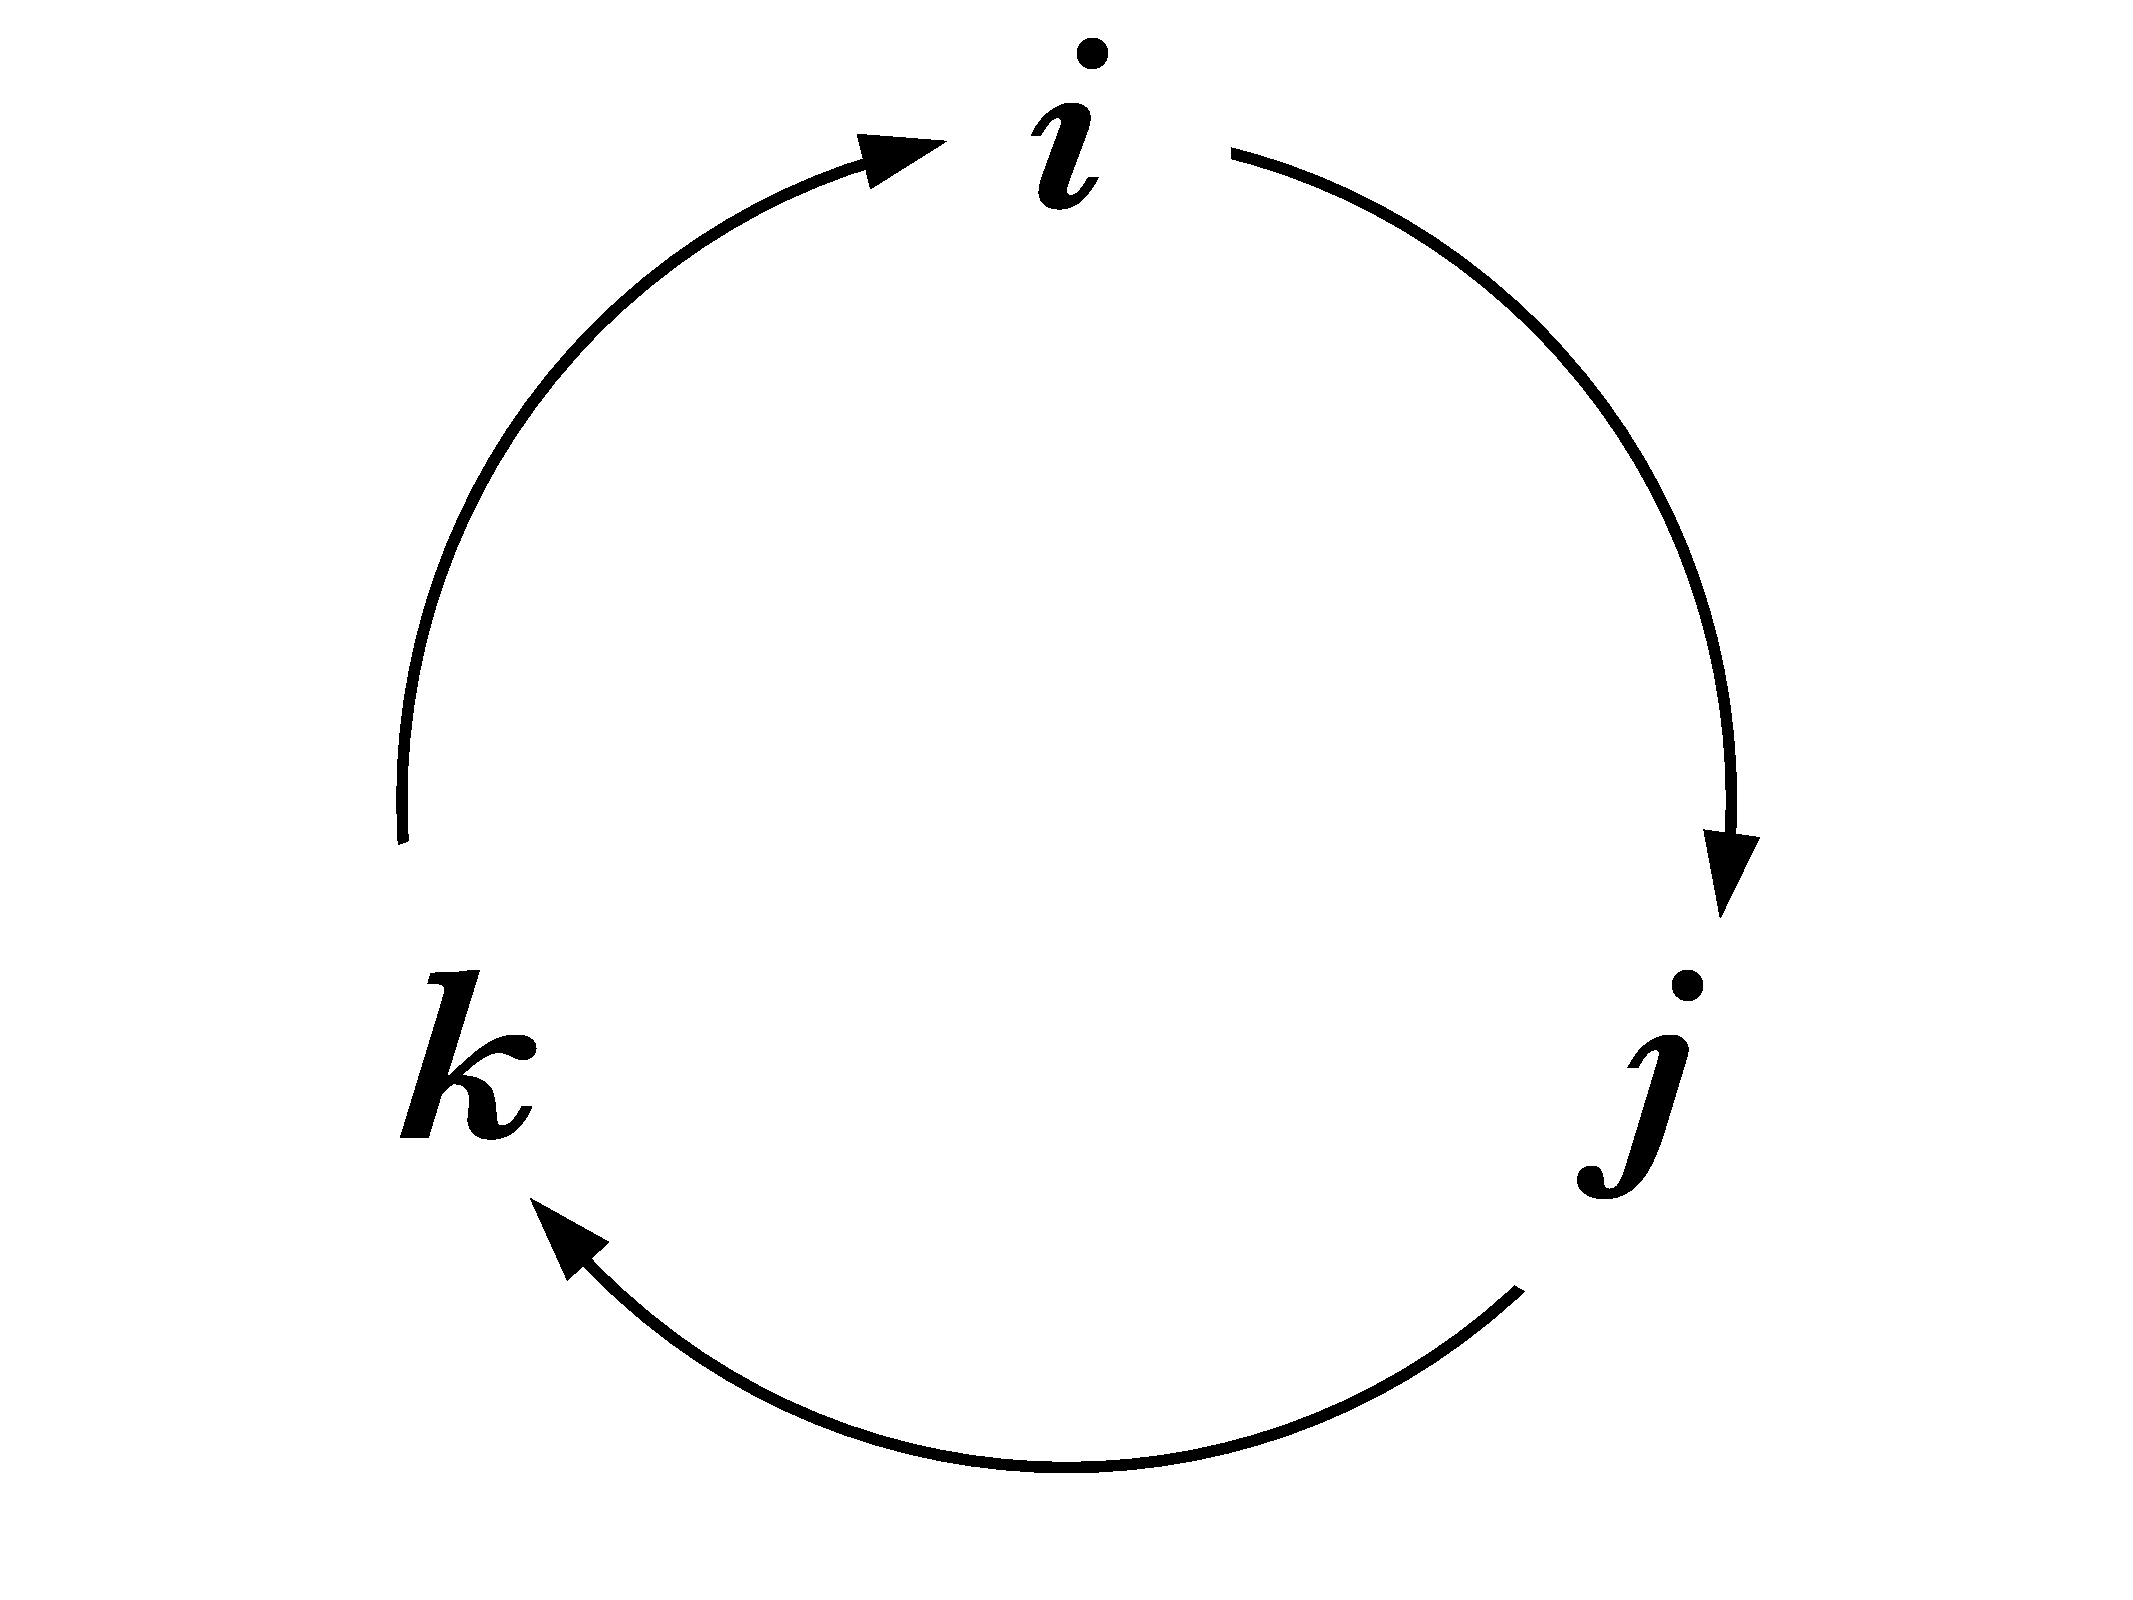
\includegraphics[width=0.2\linewidth]{Figures/quaternion_multiplication.pdf}
	\caption{Diagrama ilustrando a regra de multiplica\c c\~ao entre as unidades imagin\'arias $ \qi $, $ \qj $ e $ \qk $.}
	\label{fig:quatmult}
\end{figure}

% Moreover, $\qi$, $\qj$ and $\qk$ behave under the usual product in the same way the orthonormal base of $\mathbb{R}^3$ does with respect to the cross product, i.e. 

% \begin{equation}
% \mu_1 \mu_2 = \mu_3
% \end{equation}

% \noindent if and only if $(\mu_1, \mu_2, \mu_3)$ is a cyclical permutation of $(\qi, \qj, \qk)$ and

% \begin{equation}
% \mu_1 \mu_2 = -\mu_3
% \end{equation}

% \noindent otherwise.

Pode-se compreender $\qi, \qj$ e $\qk$ como unidades imagin\'arias ortogonais, gerando o espa\c co (tridimensional) das \emph{partes imagin\'arias} dos quat\'ernios,
\begin{equation}
\qV (q) = b\qi + c\qj + d\qk.
\end{equation}
A \emph{parte real} de um quat\'ernio \emph{q} \'e, naturalmente, definida como
\begin{equation}
S(q) = a.
\end{equation}

A parte imagin\'aria \'e comumente tamb\'em chamada de \emph{parte vetorial}, enquanto a parte real pode ser referida como \emph{parte escalar}. Um quat\'ernio com parte real nula \'e dito \emph{puro} --- o conjunto dos quais pode ser representado por $\qV(\mathbb{H})$ ---, e pode-se definir o produto vetorial entre quat\'ernios puros em analogia \`aquele usado em $\mathbb{R}^3$, i.e se $v_1 = b_1\qi + c_1\qj + d_1\qk$ e $v_2 = b_2\qi + c_2\qj + d_2\qk$, ent\~ao
\begin{equation}
v_1 \times v_2 = 
\begin{vmatrix}
\qi & \qj & \qk\\ 
b_1 & c_1 & d_1\\ 
b_2 & c_2 & d_2
\end{vmatrix}.
\end{equation}

Pela semelhan\c ca entre o conjunto $ \mathbb{R}^3 $, munido do produto vetorial, e o conjunto dos quat\'ernios puros, munido do produto vetorial entre quat\'ernios, eventualmente iremos nos referir a $\qi, \qj$ e $\qk$ como \emph{eixos}. O termo invoca a interpreta\c c\~ao destas unidades imagin\'arias como sendo eixos coordenados do espa\c co tridimensional de quat\'ernios puros.

A analogia com as opera\c c\~oes vetoriais em $\mathbb{R}^3$ aplica-se tamb\'em \`a defini\c c\~ao de produto interno entre quat\'ernios puros $v_1 = b_1\qi + c_1\qj + d_1\qk$ e $v_2 = b_2\qi + c_2\qj + d_2\qk$, a saber,
\begin{equation}
\langle v_1, v_2 \rangle =
b_1 b_2 + c_1 c_2 + d_1 d_2.
\end{equation}

A soma e o produto entre quat\'ernios permitem a distributividade (do produto em rela\c c\~ao \`a soma) e a associatividade, bastando respeitar as rela\c c\~oes em (\ref{eq:fund_rel}). Ou seja, se $q_1 = a_1 + b_1\qi + c_1\qj + d_1\qk$ e $q_2 = a_2 +  b_2\qi + c_2\qj + d_2\qk$, ent\~ao a soma \'e simplesmente dada por
\begin{equation}
q_1 + q_2 = (a_1 + a_2) + (b_1 + b_2)\qi + (c_1 + c_2)\qj + (d_1 + d_2)\qk,
\end{equation}
enquanto o produto \'e
\begin{equation}
\label{eq:q_prod}
\begin{aligned}
q_1 q_2 = &  \ (a_1 + b_1\qi + c_1\qj + d_1\qk) (a_2 +  b_2\qi + c_2\qj + d_2\qk)  \\ 
= & \ (a_1 a_2 - b_1 b_2 - c_1 c_2 - d_1 d_2)  \\
& + \qi (b_1 a_2 + a_1 b_2 - d_1 c_2 + c_1 d_2)  \\
& + \qj (c_1 a_2 + d_1 b_2 + a_1 c_2 - b_1 d_2)  \\
& + \qk (d_1 a_2 - c_1 b_2 + b_1 c_2 + a_1 d_2).
\end{aligned}
\end{equation}

Finalmente, pode-se notar que o produto entre quat\'ernios em  (\ref{eq:q_prod}) pode ser escrito em termos das partes escalar e vetorial, como
\begin{equation}
\label{eq:prod_vectors}
\begin{aligned}
q_1 q_2 = & \ S(q_1)S(q_2) - \langle\qV(q_1), \qV(q_2)\rangle \\
& + S(q_1) \qV(q_2) + S(q_2)\qV(q_1) + \qV(q_1) \times \qV(q_2).
\end{aligned}
\end{equation}
Da falta de comutatividade no produto vetorial, v\^e-se nesta equa\c c\~ao mais uma demonstra\c c\~ao de que o produto entre quat\'ernios \'e n\~ao-comutativo.

A conjuga\c c\~ao de um quat\'ernio $ q $, assim como nos complexos, \'e obtida pela troca de sinal de sua parte vetorial, $ \bar{q} \overset{\Delta}{=} S(q) - V(q) $. A defini\c c\~ao de norma, por sua vez, assemelha-se \`a de vetores em $ \mathbb{R}^4 $: $ |q| \overset{\Delta}{=} \sqrt{a^2 + b^2 + c^2 + d^2} $. Do exposto, e de (\ref{eq:prod_vectors}), percebe-se que $ |q|^2 = \bar{q} q = q \bar{q} $. Um quat\'ernio \'e \emph{unit\'ario} se $ |q| = 1 $, e o inverso de um quat\'ernio \'e encontrado em termos de seu conjugado e norma atrav\'es de
\begin{equation}
q^{-1} = \frac{\bar{q}}{|q|^2}.
\end{equation}

Da analogia entre os quat\'ernios puros e os elementos de $ \mathbb{R}^3 $, \'e natural falar em \emph{perpendicularidade} entre quat\'ernios puros. Dados $ \qmu,  \qnu \in \qV(\mathbb{H})$, percebe-se que s\~ao \emph{ortogonais} (i.~e. est\~ao associados a vetores ortogonais de $ \mathbb{R}^3 $) --- escreve-se $ \qmu \perp \qnu $ --- se e somente se
\begin{equation}
S(\qmu \qnu) = \langle \qmu, \qnu \rangle = 0.
\tag{$ \iff \qmu \perp \qnu $}
\end{equation}
Uma vez que, para dois quat\'ernios puros, unit\'arios e ortogonais $ \qmu $ e $ \qnu $, tem-se de (\ref{eq:prod_vectors}) que $ \qmu \qnu  = \qmu \times \qnu$, ent\~ao $ \qmu \qnu \perp \qmu $ e $ \qmu \qnu \perp \qnu $. Como $ (\qmu, \qnu, \qmu \qnu) $ \'e uma tripla de quat\'ernios puros, unit\'arios e ortogonais, eles formam uma base para $ \qV (\mathbb{H}) $. \'E poss\'ivel, portanto, reescrever (\ref{eq:q}) como
\begin{equation}
\label{eq:quat_generalizado}
q = a + b'\qmu + c'\qnu + d'\qmu \qnu,
\end{equation}
$a, b', c', d' \in \mathbb{R}$,
que representa um \emph{quat\'ernio generalizado}. Os ditos \emph{quat\'ernios de Hamilton} s\~ao aqueles escritos em termos da base can\^onica $ (1, \qi, \qj, \qk) $.


Al\'em da forma cartesiana em (\ref{eq:q}), os quat\'ernios permitem dois tipos de formas polares. A \emph{forma de Euler} \cite{ell2014quaternion} de um quat\'ernio \'e comumente expressa como
\begin{equation}
\label{eq:euler}
q = |q| e^{\qmu \theta} = |q|\cos \theta + |q|\qmu \sen \theta,
\end{equation}
em que $ \qmu $ \'e um quat\'ernio puro unit\'ario, paralelo \`a parte vetorial de $ q $.

Outra forma polar encontrada na literatura \cite{flamant2017time} \'e
\begin{equation}
q = |q| \exp (\qi \theta) \exp (-\qk \chi) \exp (\qj \varphi),
\end{equation}
em que os par\^ametros de fase, chamados de \^angulos de Euler, s\~ao \emph{quase unicamente} definidos sob o intervalo $ (\theta, \chi, \varphi) \in [-\pi/2, \pi/2] \times [-\pi/4, \pi/4] \times [-\pi, \pi[ $. Quando $ \chi = \pm \pi/4 $, o que equivale ao fen\^omeno do \emph{gimbal lock}, a fase do quat\'ernio n\~ao \'e bem definida.

Como consequ\^encia de (\ref{eq:euler}), \'e importante notar que todo quat\'ernio unit\'ario puro \'e uma raiz quadrada da unidade. Seja, por exemplo, o quat\'ernio unit\'ario puro $ \mathbf{\nu} $. De (\ref{eq:euler}),
\begin{equation}
%\label{key}
\mathbf{\nu} = |\mathbf{\nu}| e^{\mathbf{\nu} \theta},
\end{equation}
mas como $ |\mathbf{\nu}| = 1 $, ent\~ao
\begin{equation}
%\label{key}
\mathbf{\nu} = e^{\mathbf{\nu} \theta} \Rightarrow \theta = \pi,
\end{equation}
portanto,
\begin{equation}
%\label{key}
\mathbf{\nu}^2 = \left( e^{\mathbf{\nu}\pi} \right)^2 = e^{\mathbf{\nu} 2\pi} = 1.
\end{equation}

Esta propriedade de todo quat\'ernio puro unit\'ario $ \qmu $ leva ao fato de que os n\'umeros da forma $ a + \qmu b  $ formam um conjunto isomorfo aos n\'umeros complexos. Por esta raz\~ao, representaremos este conjunto por $ \mathbb{C}_{\qmu} \overset{\Delta}{=} \{ a + \qmu b \ |\  a, b \in \mathbb{R} \}$ ($ \mathbb{C}_{\qi} $ indica, portanto, o conjunto usual dos complexos).

Todo quat\'ernio $ q = a + b\qi + c\qj + d\qk \in \mathbb{H} $ pode ser representado segundo sua \emph{decomposi\c c\~ao simpl\'etica},
\begin{equation}
q = q^{(s)} + q^{(p)} \qj, \quad q^{(s)}, q^{(p)} \in \mathbb{C}_{\qi},
\end{equation}
em que $ q^{(s)} = a + b\qi $ e $ q^{(p)} = c + d\qi $ s\~ao frequentemente chamados de parte \emph{simplex} e \emph{perplex}, respectivamente. Perceba que essas duas componentes s\~ao n\'umeros complexos usuais. De forma geral, a decomposi\c c\~ao pode ser feita ao longo de um eixo diferente de $ \qi $: sejam $ \qmu $ e $ \qnu $ quat\'ernios puros unit\'arios e \emph{ortogonais}, ent\~ao o quat\'ernio $ q $ pode ser decomposto como
\begin{equation}
\label{eq:decomposicao}
q = q^{(s)} + q^{(p)} \qnu, \quad q^{(s)}, q^{(p)} \in \mathbb{C}_{\qmu}.
\end{equation}
Esta decomposi\c c\~ao tem grande import\^ancia no c\'alculo da QDFT (se\c c\~ao \ref{sec:QFT}) e na an\'alise de matrizes quaterni\^onicas (ca\'itulo \ref{ch:QGSP}).

Dois quat\'ernios $ q $ e $ r $ s\~ao ditos \emph{similares} se existe um quat\'ernio n\~ao-nulo $ v $ tal que $ v^{-1}q v = r $. Neste caso, pode-se escrever $ q \sim r $. A similaridade \'e uma rela\c c\~ao de equival\^encia entre quat\'ernios \cite{zhang1997quaternions}, e pode-se notar que todos os elementos de uma mesma classe de equival\^encia possuem a mesma norma, pois $ |v^{-1}q v| = |v^{-1}| \cdot |q| \cdot |v| = |q| $. Importa mencionar uma valiosa propriedade das transforma\c c\~oes de similaridade entre quat\'ernios, respons\'avel por sua grande aplica\c c\~ao na mec\^anica e na ind\'ustria da computa\c c\~ao gr\'afica. Trata-se da opera\c c\~ao de rota\c c\~ao no espa\c co 3D: dados $ v,x \in \mathbb{H} $, $ v = |v| e^{\qmu \alpha}$, a transforma\c c\~ao de similaridade
\begin{equation}
\label{eq:rotacao}
\phi_v(x) = v x v^{-1}
\end{equation}
produz a rota\c c\~ao da parte vetorial (imagin\'aria) de $ x $ em torno do eixo $ \qmu $ (que tem a mesma dire\c c\~ao da parte vetorial de $ v $) de um \^angulo $ 2\alpha $ \cite{ward2012quaternions}, seguindo a regra da m\~ao direita.


\section{On the theory of quaternion matrices}

When analyzing the eigenstructure and subsequent fractionarization of the QDFT matrix, the eigendecomposition of the DFT and the eigenvector sharing served as a convenient shortcut. In order to build the results in QGSP, however, it is required to dive into more general properties of quaternion matrices. The symplectic decomposition, already presented in (\ref{eq:decomposicao}), plays an important role in that matter, specialy for its use in defining the complex\textit{ adjoint matrix}.

\begin{definition}[Complex adjoint matrix \cite{zhang1997quaternions}]
Given $ \mathbf{A} \in \mathbb{H}^{n \times n} $, with symplectic decomposition $ \mathbf{A}_1 + \mathbf{A}_2 \qj$, $ \mathbf{A}_1,\mathbf{A}_2 \in \mathbb{C}^{n \times n} $, its complex adjoint matrix is defined as
\begin{equation}
\rchi_{A} \overset{\Delta}{=}
\begin{pmatrix}
\mathbf{A}_1 & \mathbf{A}_2\\ 
- \overline{\mathbf{A}}_2 & \overline{\mathbf{A}}_1
\end{pmatrix}.
\end{equation}
\end{definition}

In the following theorems, Zhang brings fundamental results for building QGSP.

\begin{theorem}[Part of Theorem 4.2 in
\cite{zhang1997quaternions}
]
\label{th:equiv01}
Given the matrix $ \mathbf{A} \in \mathbb{H}^{n \times n} $, the following sentences are equivalent:

\begin{itemize}[noitemsep]
\item $ \rchi_{AB} = \rchi_{A} \rchi_{B} $,
\item $ \rchi_{A^{-1}} = \rchi_{A}^{-1}$, if $ \mathbf{A}^{-1} $ exists,
\item $ \rchi_{A}$ is unitary, hermitian or normal if and only if so is $ \mathbf{A} $.
\end{itemize}

\end{theorem}

\begin{theorem}[Part of Theorem 4.3 in
\cite{zhang1997quaternions}
]
\label{th:equiv02}
Given the matrix $ \mathbf{A} \in \mathbb{H}^{n \times n} $, the following sentences are equivalent:

\begin{itemize}[noitemsep]
\item $\mathbf{A}$ is invertible.
\item $\mathrm{det}(\rchi_A) \neq 0$, i.e. $\rchi_{A}$ is invertible.
\end{itemize}

\end{theorem}


% Em \cite[Teoremas 4.2 e 4.3]{zhang1997quaternions}, Zhang traz alguns resultados interessantes da literatura a respeito de $ X_A $, dos quais cabe mencionar:
% \begin{itemize}[noitemsep]
% \item $ \rchi_{AB} = \rchi_{A} \rchi_{B} $,
% \item $ \rchi_{A^{-1}} = \rchi_{A}^{-1}$, se $ \mathbf{A}^{-1} $ existir,
% \item $ \rchi_{A}$ \'e unit\'aria, hermitiana ou normal se e somente se $ \mathbf{A} $ tamb\'em o for.
% \end{itemize}

A matriz complexa adjunta serve como uma representa\c c\~ao complexa da matriz quaterni\^onica e, diferente de outras representa\c c\~oes matriciais em $ \mathbb{C} $ ou $ \mathbb{R} $, esta permite estabelecer um v\'inculo entre o espectro de $ \rchi_{A} $ e o de $ \mathbf{A} $, como ser\'a discutido adiante.

\subsection{Autovalores}

Uma vez que a multiplica\c c\~ao sobre os quat\'ernios n\~ao \'e comutativa, faz-se necess\'ario distinguir os \emph{autovalores \`a esquerda} e os \emph{autovalores \`a direita} de uma matriz $ \mathbf{A} \in \mathbb{H}^{n \times n} $,
\begin{align*}
\mathbf{A} \mathbf{v} &= \mathbf{v} \lambda, \tag{autovalor \`a direita} \\
\mathbf{A} \mathbf{v} &= \lambda \mathbf{v}.  \tag{autovalor \`a esquerda}
\end{align*}

Uma vez que o problema dos autovalores \`a direita foi mais compreendido do que daqueles \`a esquerda, e possui mais resultados \cite[Cap. 5]{zhang1997quaternions}, restringiremos a an\'alise aos autovalores \`a direita. Quando n\~ao for mencionado, estes ser\~ao chamados apenas de \emph{autovalores} da matriz quaterni\^onica.

\'E importante mencionar que uma matriz quaterni\^onica possui um n\'umero \emph{finito} de autovalores se, e somente se, s\~ao todos reais. Do contr\'ario, cada autovalor pertence a uma classe de similaridade, segundo a transforma\c c\~ao $ \lambda_1 = q^{-1} \lambda_2 q $, contendo \emph{infinitos} outros quat\'ernios que tamb\'em s\~ao autovalores da matriz. Seja, por exemplo, o autovalor $ \lambda $ da matriz $ \mathbf{A} $, associado ao autovetor $ \mathbf{v} $. Ent\~ao,
\begin{equation}
\begin{aligned}
\label{eq:similar}
\mathbf{A} \mathbf{v} &= \mathbf{v} \lambda \\
\mathbf{A} \mathbf{v} q &= \mathbf{v} \lambda q = \mathbf{v} q q^{-1} \lambda q \\
\mathbf{A} (\mathbf{v} q) &= (\mathbf{v} q) q^{-1} \lambda q,
\end{aligned}
\end{equation}
de modo que $ q^{-1} \lambda q $ \'e um autovalor associado ao autovetor $ \mathbf{v}q $, com $ q \in \mathbb{H}^\ast $.

\subsection{Rotacionando autovalores}
\label{subsec:rotacionando}

Pretende-se aplicar a diagonaliza\c c\~ao de matrizes quaterni\^onicas no contexto da an\'alise espectral do operador de deslocamento sobre um grafo com pesos quaterni\^onicos. Neste caso, os seus autovalores poder\~ao ser interpretados como frequ\^encias. O problema do ordenamento destas frequ\^encias, bem definido para o caso de matrizes laplacianas ou de adjac\^encia reais, pode-se mostrar desafiador ao lidar com autovalores quaterni\^onicos\footnote{Mesmo ao se utilizar o racioc\'inio do teorema \ref{th:02}, da subse\c c\~ao \ref{subsec:autovetores_XA}, em que os autovalores s\~ao obtidos diretamente com valores complexos, \'e poss\'ivel que, em alguns problemas, tenha-se em m\~aos os autovalores quaterni\^onicos, caso em que o procedimento aqui descrito \'e \'util. De toda forma, a rota\c c\~ao de autovalores \'e uma ferramenta valiosa, sendo utilizada, por exemplo, na demonstra\c c\~ao do teorema \ref{th:02}.}.
Uma hip\'otese a se analisar \'e que este ordenamento seja facilitado ao se encontrar, para cada autoclasse, o respectivo autovalor \emph{complexo}. Como feito em \cite[Eq. (4.8)]{de2002quaternioic}, trata-se de transformar a equa\c c\~ao de autovetor quaterni\^onica em outra equivalente, com autovalor complexo, a partir da rota\c c\~ao da parte imagin\'aria (\emph{rephasing}) de cada autovalor no espa\c co $ \qi, \qj, \qk $ at\'e alinh\'a-la com $ \qi $. Em suma, utilizando a propriedade de rota\c c\~ao no espa\c co $ \qV (\mathbb{H}) $ em (\ref{eq:rotacao}), parte-se de
\begin{equation}
\label{eq:01}
\mathbf{A} \mathbf{v} = \mathbf{v} \lambda
\end{equation}
para chegar em
\begin{equation}
\label{eq:02}
\mathbf{A} (\mathbf{v} q) = (\mathbf{v} q) q^{-1} \lambda q,
\end{equation}
com a restri\c c\~ao $ q^{-1} \lambda q \in \mathbb{C}_{\qi} $.

\begin{quotation}
\begin{example}
	\upshape
	Consideremos, por exemplo, um caso em que $ \lambda = 3\qi + \qk $ e $ \mathbf{v} $ tem comprimento $ n=2 $,
	\begin{equation}
	%\label{key}
	\mathbf{v} =\begin{pmatrix}
	1 +  \qi\\
	2 \qj + \qk
	\end{pmatrix}.
	\end{equation}
	
	A matriz quaterni\^onica $ \mathbf{A} $ que satisfaz
	\begin{equation}
	\label{eq:03}
	\mathbf{A} \mathbf{v} = \mathbf{v} \lambda,
	\end{equation}
	com a restri\c c\~ao arbitr\'aria de possuir a primeira coluna igual a $ (1 \quad 1)^T $ \'e
	\begin{equation}
	%\label{key}
	\mathbf{A} =
	\begin{pmatrix}
	1 & - \frac{1}{5} + \frac{3}{5} \qi + 2 \qj \\
	1 & -3 \qi + \qj
	\end{pmatrix}.
	\end{equation}
	
	De posse das vari\'aveis da equa\c c\~ao (\ref{eq:01}), pode-se partir para ilustrar o procedimento de \emph{rephasing}, ou rota\c c\~ao da parte imagin\'aria, descrito em (\ref{eq:02}). A ideia \'e utilizar um quat\'ernio unit\'ario para rotacionar $ \lambda $ no espa\c co quaterni\^onico e, neste exemplo particular, rotacion\'a-lo no plano $ \qi \qk $ por um \^angulo $ \theta = \tan^{-1} \frac{1}{3} $ radianos em dire\c c\~ao ao eixo $ \qi $. Como ilustrado na Fig. \ref{fig:quat3ik}, o resultado esperado \'e um n\'umero $ z \in \mathbb{C}_{\qi} $.
	
	
	\begin{figure}
		\centering
		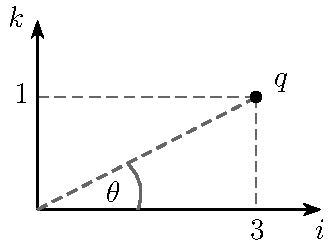
\includegraphics[width=0.3\linewidth]{Figures/quaternion01.pdf}
		\caption{Representa\c c\~ao de $ \lambda = 3\qi + \qk $ no plano $ \qi \qk $.}
		\label{fig:quat3ik}
	\end{figure}
	
%	Utilizaremos a propriedade de rota\c c\~ao da parte vetorial de quat\'ernios, em (\ref{eq:rotacao}).
	Uma vez que o plano $ \qi \qk $ \'e ortogonal a $ \qj $ (lembrando que os tr\^es eixos s\~ao orientados positivamente), a rota\c c\~ao desejada neste plano, positivamente orientada em torno de $ \qj $ e obtida por inspe\c c\~ao da Fig. \ref{fig:quat3ik}, \'e realizada pelo quat\'ernio
	\begin{equation}
	\label{eq:04}
	v = e^{\qj \alpha}, \quad 2\alpha = \theta = \tan^{-1} \frac{1}{3},
	\end{equation}
	utilizando o mapeamento $ \lambda \mapsto v \lambda v^{-1} $ em (\ref{eq:rotacao}).
	
	Uma vez que a transforma\c c\~ao desejada \'e $ \lambda \mapsto q^{-1} \lambda q $, ent\~ao
	\begin{equation}
	%\label{key}
	q = v^{-1} = e^{- \qj \alpha} = e^{- \qj \frac{\theta}{2}}.
	\end{equation}
	
	%It is a known property that ({\color{red}(retirado do artigo ``quat\'ernio rotation intuition'' do math.stack\-exchange, buscar melhor fonte!)}) ``if $ v = e^{\qmu \alpha} = \cos \alpha + \qmu \sin \alpha$, then the mapping $ x \mapsto v x v^{-1} $ will rotate purely imaginary quat\'ernios around the axis $ \mathbb{R} \qmu $ by the angle $ 2\alpha $ according to the right-hand rule''.
	
	Como forma de confer\^encia, encontremos o valor de $ \alpha $ que resulta em $ q^{-1} \lambda q \in \mathbb{C}_{\qi} $. Como $ v = q^{-1} = \cos \alpha + \qj \sin \alpha $,
	\begin{equation}
	%\label{key}
	\begin{aligned}
	%\label{key}
	q^{-1} \lambda &= (\cos \alpha + \qj \sin \alpha)(3 \qi + \qk)\\
	&= \qi(3 \cos \alpha + \sin \alpha) + \qk(\cos \alpha - 3 \sin \alpha). \\
	q^{-1} \lambda q &= [\qi(3 \cos \alpha + \sin \alpha) + \qk(\cos \alpha - 3 \sin \alpha)] (\cos \alpha - \qj \sin \alpha) \\
	&= \qi (3 \cos 2\alpha + \sin 2\alpha) + \qk(\cos 2\alpha - 3 \sin 2\alpha).
	\end{aligned}
	\end{equation}
	
	Portanto, $ q^{-1} \lambda q \in \mathbb{C}_{\qi} $ se e somente se
	\begin{equation}
	%\label{key}
	\begin{aligned}\textbf{}
	\cos 2\alpha - 3 \sin 2\alpha &= 0 \\
	2\alpha &= \tan^{-1} \frac{1}{3},
	\end{aligned}
	\end{equation}
	como inferido em (\ref{eq:04}).
	
Assim, o quat\'ernio puro unit\'ario $ q = e^{- \qj \alpha} $, $ \alpha = - \displaystyle \nicefrac{1}{2} \tan^{-1} \nicefrac{1}{3} $, \'e capaz de fazer $ q^{-1} \lambda q \in \mathbb{C}_{\qi}$, de modo que a equa\c c\~ao de autovalor em (\ref{eq:03}) pode ser reescrita como em (\ref{eq:02}),
	\begin{equation}
	%\label{key}
	\mathbf{A} \underbrace{\begin{pmatrix}
		cos \alpha + \qi \sin \alpha - \qj \sin \alpha - \qk \sin \alpha \\
		2 \sin \alpha + \qi \sin \alpha + \qj 2 \cos \alpha + \qk \cos \alpha
		\end{pmatrix}}_{= \mathbf{v} q} =
	(\mathbf{v} q) \cdot \underbrace{\qi (3 \cos 2\alpha + \sin 2\alpha)}_{= q^{-1} \lambda q}.
	%\underbrace{3.162 \qi}_{= \bar{u} q u}.
	\end{equation}
\end{example}
\end{quotation}

\subsection{Diagonalizabilidade}
\label{subsec:autovetores_XA}

Quanto ao problema de determinar se uma matriz quaterni\^onica \'e \emph{diagonaliz\'avel}, h\'a que se observar que, diferentemente do caso complexo, ter todos os autovalores distintos n\~ao \'e condi\c c\~ao suficiente para diagonalizabilidade. Tomemos o contra-exemplo dado por Zhang \cite[Exemplo 7.4]{zhang1997quaternions}, a matriz
\begin{equation}
\mathbf{A} =
\begin{pmatrix}
\qi & 1\\ 
0 & \qj
\end{pmatrix}.
\end{equation}

Embora possua autovalores distintos -- $ \qi $ e $ \qj $, pois s\~ao as entradas diagonais de uma matriz triangular --, os respectivos autovetores da matriz $ \mathbf{A} $ n\~ao formam um conjunto linearmente independente. Pode-se verificar, por exemplo, que um autovetor associado a $ \qi $ \'e $ (1, 0)^T $, enquanto um associado a $ \qj $ \'e $ (\qi + \qj, 0)^T $. A raz\~ao deles serem linearmente dependentes \'e o fato, mencionado anteriormente, de que para todo autovalor e autovetor $ \lambda $ e $ \mathbf{v} $ de uma matriz quaterni\^onica, tem-se $ q^{-1}\lambda q $ e $ \mathbf{v}q $ como outros autovalor e autovetor, com $ q \in \mathbb{H}^\ast $. Ou seja, dois autovalores \emph{similares} est\~ao sempre associados aos mesmos autovetores, a menos de um fator de escala. Por isso, quat\'ernios similares s\~ao ditos pertencentes \`a mesma \emph{autoclasse} \cite{de2000right}. Para que o conjunto de autovetores associados aos autovalores distintos de uma matriz quaterni\^onica sejam linearmente independentes, portanto, estes autovalores \textbf{n\~ao} podem ser similares.  Concluindo o exemplo dado, pode-se mostrar que $ \qi $ e $ \qj $ s\~ao similares: $ \qj = q \qi q^{-1} $, para $ q \in \{ a - a\qi - a\qj + a\qk \ | \ a\in \mathbb{R}^\ast \} $.

O teorema \ref{th:02} relaciona a autodecomposi\c c\~ao de uma matriz e de sua complexa adjunta, fornecendo um princ\'ipio \'util para o estudo da autoestrutura de matrizes quaterni\^onicas.


\begin{figure}
\centering
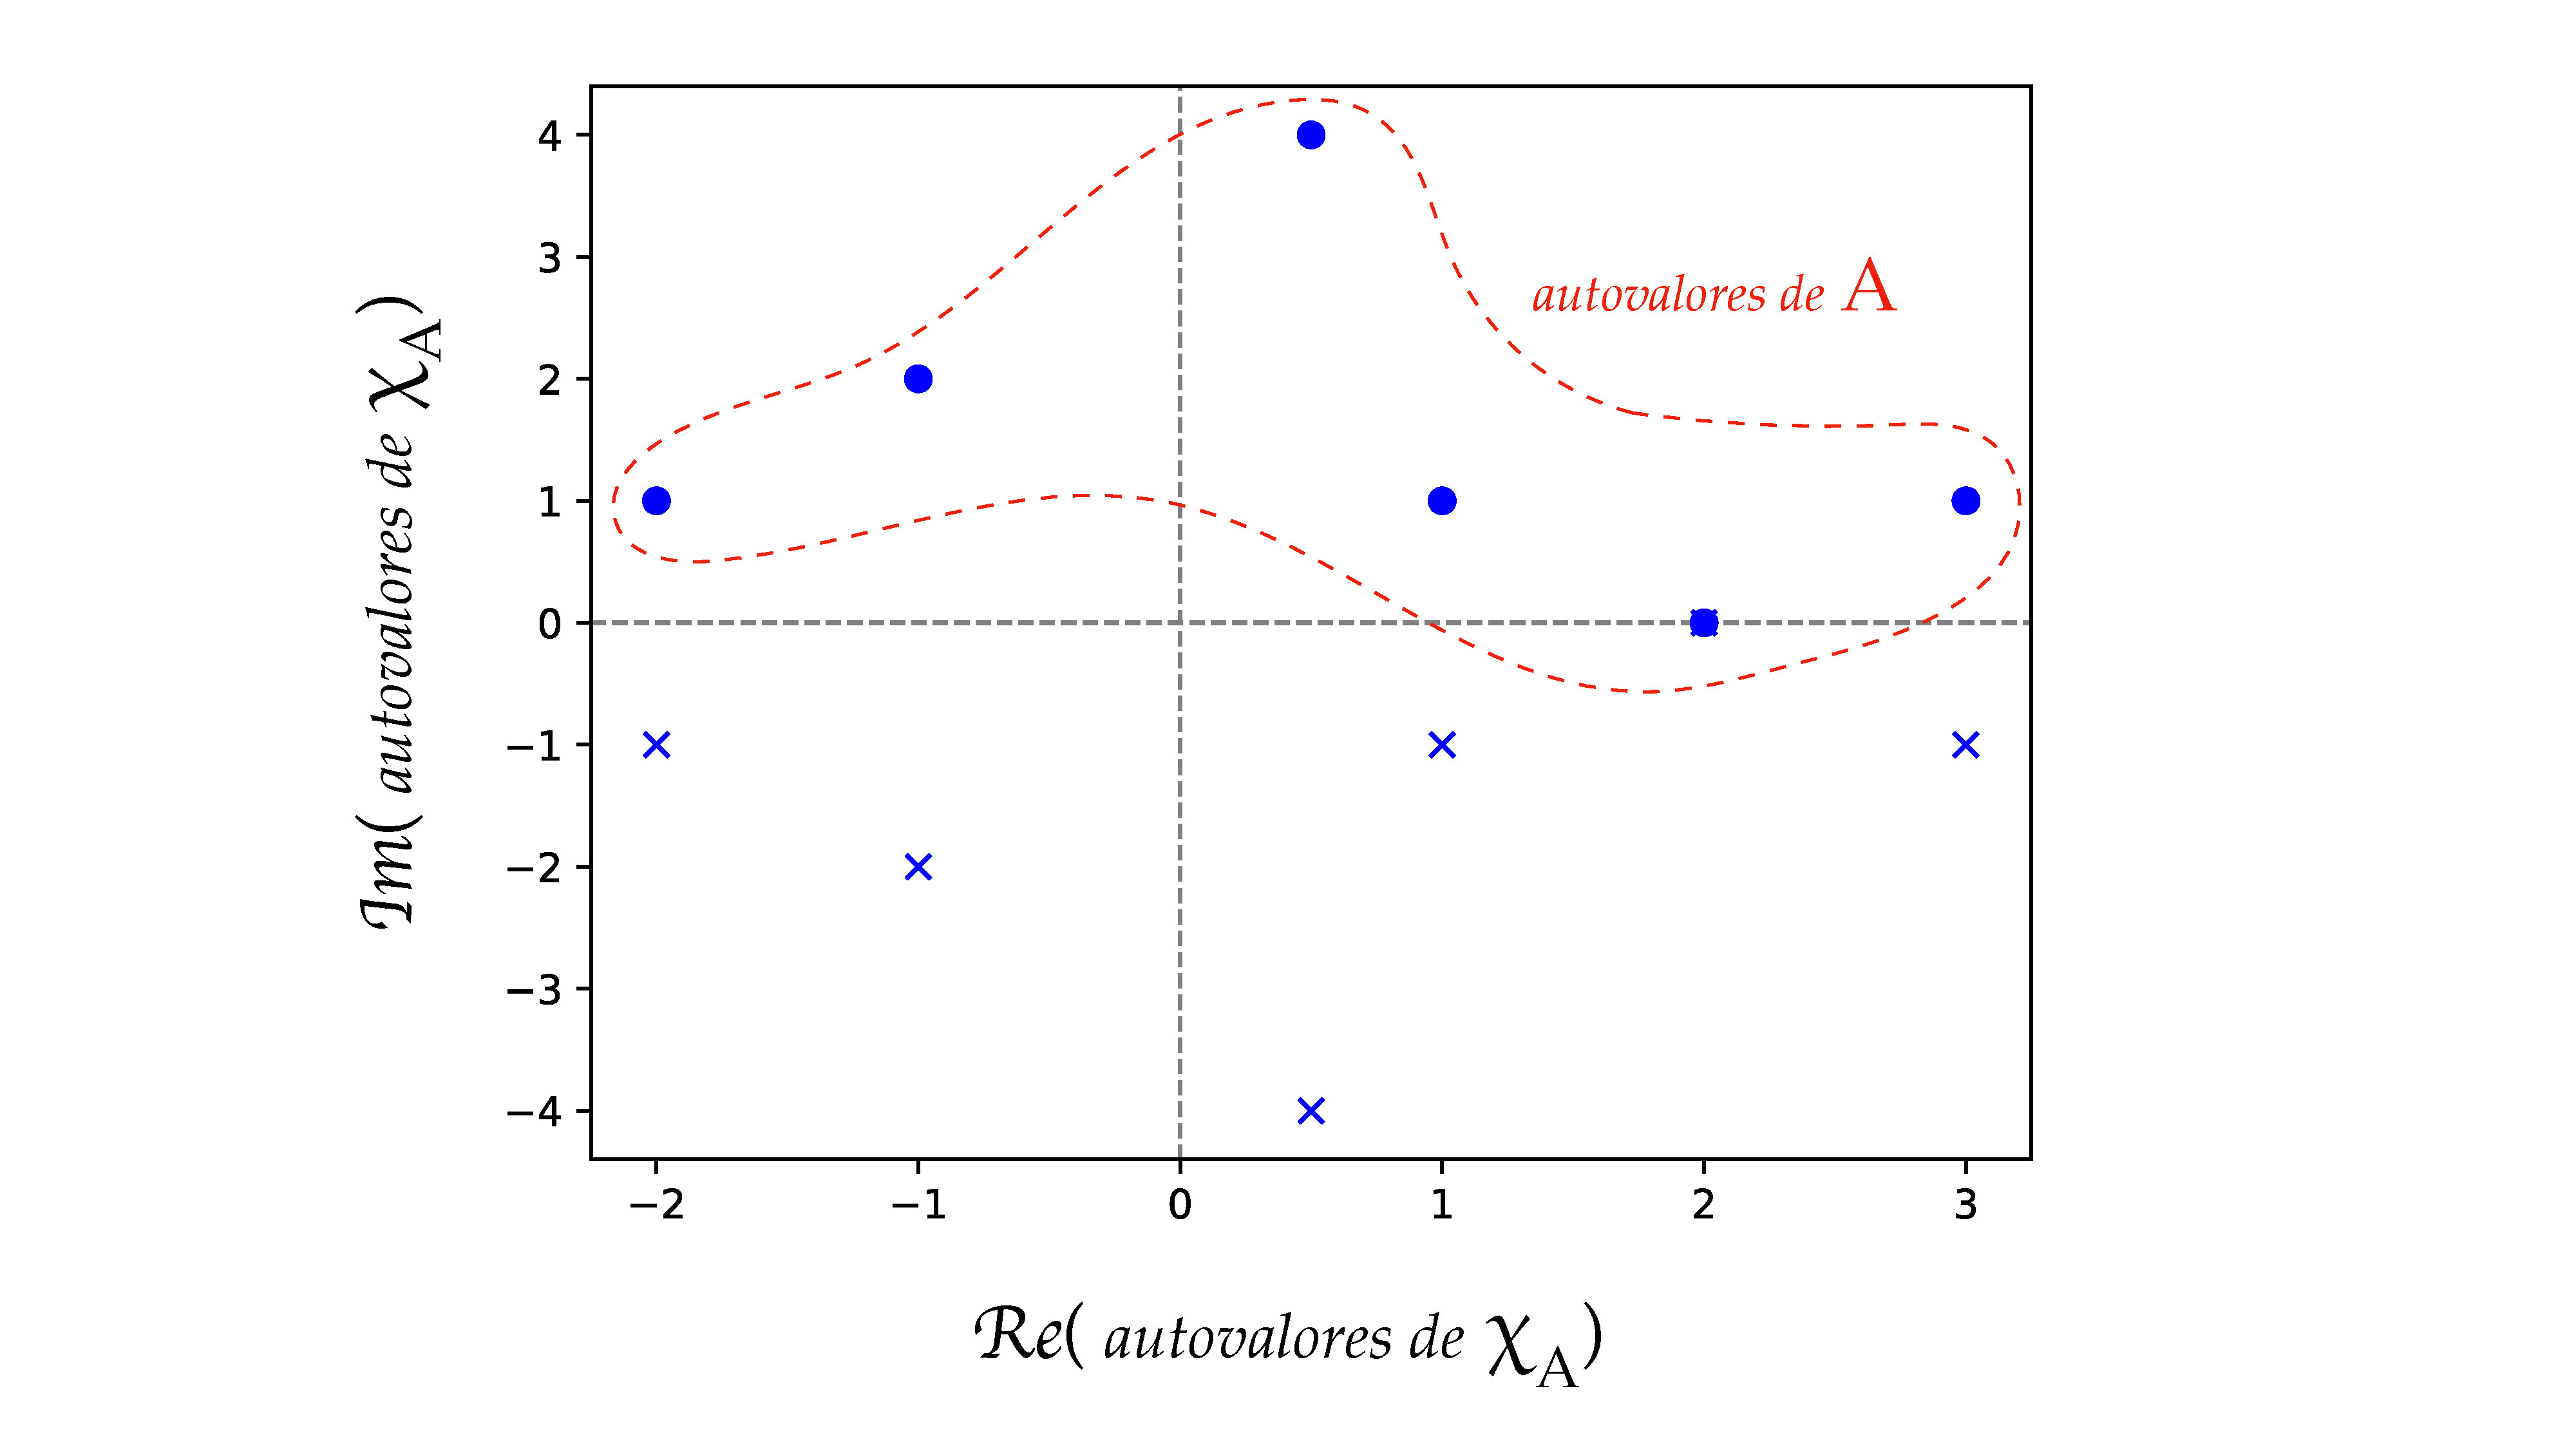
\includegraphics[width=0.6\linewidth]{Figures/complex_adjoint_eigvals_PT.pdf}
\caption{\emph{Autovalores padrão} de uma matriz $ \mathbf{A} $ quaterni\^onica, indicados como um subconjunto dos autovalores de sua respectiva matriz complexa adjunta.}
\end{figure}


\begin{theorem}[\cite{zhang1997quaternions}]
\label{th:02}
Toda matriz $ A \in \mathbb{H}^{n \times n} $ tem exatamente $ n $ autovalores complexos
%(\`a direita),
%que s\~ao iguais aos autovalores de $ \rchi_A $, sua complexa adjunta,
com parte imagin\'aria n\~ao-negativa. Estes s\~ao ditos os \emph{autovalores padr\~ao} de $ \mathbf{A} $ e s\~ao um subconjunto dos $ 2n $ autovalores de $ \rchi_A $.
\end{theorem}

\begin{proof}
Como demonstrado no ap\^endice \ref{ch:AppendixA}, a partir da equa\c c\~ao de autovalor quaterni\^onica
\begin{equation}
\mathbf{A} \mathbf{v} = \mathbf{v} \lambda
\end{equation}
em que se pode assumir, sem perda de generalidade, que $ \lambda \in \mathbb{C} $, pode-se chegar \`a equa\c c\~ao equivalente
\begin{equation}
\begin{pmatrix}
\mathbf{A}_1 & \mathbf{A}_2\\ 
- \overline{\mathbf{A}}_2 & \overline{\mathbf{A}}_1
\end{pmatrix}
\begin{pmatrix}
\mathbf{v}_1 \\ 
- \overline{\mathbf{v}}_2
\end{pmatrix} =
\begin{pmatrix}
\mathbf{v}_1 \\ 
- \overline{\mathbf{v}}_2
\end{pmatrix}
\lambda,
\end{equation}
envolvendo apenas vari\'aveis complexas (i.~e. as componentes da decomposi\c c\~ao de simpl\'etica de $ \mathbf{A} $ e $ \mathbf{v} $). Uma vez que
\begin{equation}
\rchi_A = 
\begin{pmatrix}
\mathbf{A}_1 & \mathbf{A}_2\\ 
- \overline{\mathbf{A}}_2 & \overline{\mathbf{A}}_1
\end{pmatrix}
\end{equation}
\'e uma matriz complexa $ 2n \times 2n $, ela possui $ 2n $ autovalores complexos (distintos ou não). Segundo \cite[Teorema 5]{lee1948eigenvalues}, seus autovalores ocorrem na forma de $ n $ pares conjugados e, por isso, a matriz $ \mathbf{A} $ possui exatamente $ n $ autovalores complexos com parte imagin\'aria n\~ao-negativa.

Os demais autovalores s\~ao redundantes. Seja $ q \in \mathbb{C}_{\qi}$ um destes autovalores. Podemos mostrar que $ q \sim \overline{q} $, pois obt\'em-se $ \overline{q} $ atrav\'es de uma rota\c c\~ao da parte imagin\'aria de $ q $ de 180$ ^\circ $ em torno do eixo $ \qj $. Utilizando o racioc\'inio exposto na subse\c c\~ao \ref{subsec:rotacionando}, com o quat\'ernio $ v = e^{\qj \frac{\pi}{2}} = \qj $ (logo $ v^{-1} = e^{- \qj \frac{\pi}{2}} = -\qj $) e o mapeamento $ q \mapsto v q v^{-1} $,
\begin{equation}
\begin{aligned}
v q v^{-1} &= \qj (q_r + q_i \qi) (-\qj) = q_r - q_i \qj \qi \qj\\
&= q_r + q_i \qi \qj \qj = q_r - q_i \qi = \overline{q}.
\end{aligned}
\end{equation}
Como dois autovalores conjugados de $ \rchi_A $ s\~ao similares, eles pertencem \`a mesma autoclasse e apontam para o mesmo conjunto linearmente dependente de autovetores. Assim, pode-se tomar sempre aquele com parte imagin\'aria nula ou n\~ao-negativa, por conven\c c\~ao.
\end{proof}

O teorema a seguir \'e outro resultado fundamental relacionando a autoestrutura de uma matriz quaterni\^onica e a de sua complexa adjunta.

\begin{theorem}[Teorema 7.4 em \cite{zhang1997quaternions}]
\label{th:diagonal}
Dadas as matrizes $ \mathbf{A}, \mathbf{B} \in \mathbb{H}^{n \times n} $, ent\~ao $ \mathbf{A} $ \'e similar a $ \mathbf{B} $ se, e somente se, $ X\rchi_A $ \'e similar a $ \rchi_B $.
\end{theorem}

\begin{corollary}
Uma matriz $  \mathbf{A} \in \mathbb{H}^{n \times n} $ \'e diagonaliz\'avel se, e somente se, $ \rchi_A $ \'e diagonaliz\'avel.
\end{corollary}
\begin{proof}
Se $ \mathbf{A} \in \mathbb{H}^{n \times n} $ \'e diagonaliz\'avel, ent\~ao \'e similar a uma matriz diagonal $ \Lambda \in \mathbb{C}^{n \times n}_{\qi} $ contendo seus autovalores padr\~ao. Do teorema \ref{th:diagonal}, segue que $ \rchi_A $ \'e similar a
\begin{equation}
\label{eq:Xlambda}
\rchi_{\Lambda} =
\begin{pmatrix}
\Lambda & \mathbf{0}\\ 
\mathbf{0} & \overline{\Lambda}
\end{pmatrix},
\end{equation}
que tamb\'em \'e uma matriz diagonal. Portanto, $ \rchi_A $ \'e diagonaliz\'avel.

Por outro lado, se $ \rchi_A $ \'e diagonaliz\'avel, ent\~ao \'e similar a uma matriz diagonal contendo os seus $ 2n $ autovalores, que aparecem em $ n $ pares complexos conjugados. Assim, sua matriz de autovalores pode ser escrita como (\ref{eq:Xlambda}), o que implica, pelo teorema \ref{th:diagonal}, que $ \mathbf{A} $ \'e similar a $ \Lambda $.
\end{proof}

\section{The quaternion Fourier transform}
\label{sec:QFT}

Ao considerar-se sinais de valores quaterni\^onicos, a literatura contempla algumas ferramentas para seu processamento, como um operador gradiente \cite{jiang2014general} e algoritmos de filtragem adaptativa \cite{jiang2013frequency}. Nesta se\c c\~ao, no entanto, o foco ser\'a dado \`a transformada de Fourier quaterni\^onica (QFT, \emph{quaternion Fourier transform}), base para a an\'alise espectral de fun\c c\~oes hipercomplexas.

Seja $f$ uma fun\c c\~ao de valores quaterni\^onicos $f: \mathbb{R} \rightarrow \mathbb{H}$ e $\qmu \in \qV(\mathbb{H})$, $\qmu^2 = -1$. A QFT unidimensional \emph{\`a esquerda} pode ser definida pela fam\'ilia de transformadas
\begin{equation}
\mathcal{F}^L_{\mp \qmu}[f](\omega) = 
F^L_{\mp \qmu}(\omega) \overset{def}{=}
\kappa_{-} \int_{-\infty}^{\infty} e^{\mp \qmu \omega t} f(t) \mathrm{d}t.
\tag{QFT 1D \`a esquerda}
\end{equation}

Pode-se provar que a opera\c c\~ao inversa existe e \'e dada por
\begin{equation}
\mathcal{F}^{-L}_{\pm \qmu}[F^L](t) = 
f(t) =
\kappa_{+} \int_{-\infty}^{\infty} e^{\pm \qmu \omega t} F^L(\omega) \mathrm{d}\omega.
\tag{QFT 1D \`a esquerda inversa}
\end{equation}

Nas express\~oes acima, o quat\'ernio puro unit\'ario $\qmu$ indica o \emph{autoeixo} do n\'ucleo da transformada, \'e a unidade imagin\'aria de refer\^encia. Seu sinal no n\'ucleo da transformada \'e arbitr\'ario, bastando que as transforma\c c\~oes direta e inversa contenham sinais opostos. As constantes reais $\kappa_{-}$ e $\kappa_{+}$ satisfazem
\begin{equation}
\kappa_{+} \kappa_{-} = \frac{1}{2\pi},
\end{equation}
\noindent e se $\kappa_{-} = \kappa_{+}$, a transformada \'e dita unit\'aria.

%Similarly, the right-sided QFT pair is given by
%
%\begin{equation}
%\mathcal{F}^R_{\mp \mu}[f](\omega) = 
%F^R_{\mp \qmu}(\omega) \overset{def}{=}
%\kappa_{-} \int_{-\infty}^{\infty}  f(t) e^{\mp \qmu \omega t}  \mathrm{d}t.
%\tag{1D right-sided QFT}
%\end{equation}
%
%\begin{equation}
%\mathcal{F}^{-R}_{\pm \mu}[F^R](t) = 
%f(t) =
%\kappa_{+} \int_{-\infty}^{\infty} F^R(\omega) e^{\pm \qmu \omega t}  \mathrm{d}\omega.
%\tag{Inverse 1D right-sided QFT}
%\end{equation}
%
%
%Let $f_s, f_p \in \mathbb{C}_{\qmu}$ be respectively the simplex and perplex parts of the quat\'ernio-valued function $f(t)$, with respect to the unit quat\'ernio $\qnu$ so that $\qnu \perp \qmu$. Hence 
%
%\begin{align*}
%F^L(\omega) &= \kappa_{-} \int_{-\infty}^{\infty}
%e^{- \qmu \omega t} f(t) \mathrm{d}t \\
%& = 
%\kappa_{-} \int_{-\infty}^{\infty}
%e^{- \qmu \omega t} f_s(t) \mathrm{d}t +
%\kappa_{-} \int_{-\infty}^{\infty}
%e^{- \qmu \omega t} f_p(t) \mathrm{d}t \qnu \\
%&= \underbrace{F^L_s (\omega)}_{\isomorphism CTFT} + \underbrace{F^L_p (\omega)}_{\isomorphism CTFT} \qnu,
%\end{align*}
%
%\noindent that is, the QFT may be computed using two continuous-time Fourier Transforms (CTFT) subsequent to symplectic decomposition of the function transformed function.

Da mesma forma como foi definida a transformada \`a esquerda, pode-se tratar da transformada \`a direita, alterando a posi\c c\~ao relativa entre a fun\c c\~ao $ f(t) $ e o n\'ucleo. O leitor deve perceber que, no caso em que o autoeixo coincide com $ \qi $, a QFT coincide com a transformada de Fourier de tempo
%\footnote{Por raz\~oes hist\'oricas, o termos \emph{tempo} e \emph{frequ\^encia} ser\~ao utilizados para se referir, respectivamente, aos dom\'inios da fun\c c\~ao original e da fun\c c\~ao transformada, muito embora em alguns cen\'arios as vari\'aveis livres n\~ao tenham tais significados (e.g. no processamento de imagens).}
cont\'inuo.

Nesta pesquisa, ter\'a mais relev\^ancia a vers\~ao da QFT em que os dom\'inios de origem e de destino da transformada s\~ao discretos, a QDFT unidimensional de eixo $ \qmu $, como definida em \cite[sec. 3.3.1]{ell2014quaternion}. Se $ \qmu $ \'e um quat\'ernio unit\'ario puro qualquer, a $ m $-\'esima componente do vetor transformado pela QDFT unit\'aria de eixo $ \qmu $ \`a esquerda \'e dada por
\begin{equation}
\label{eq:QDFT_fwd}
\widehat{v}_m = \text{QDFT}\{ \mathbf{v} \}_m \overset{\Delta}{=} \frac{1}{\sqrt{N}} \sum_{n=0}^{N-1}  \exp \left( -\qmu \frac{2\pi}{N} nm \right) v_n \in \mathbb{C}_{\qmu},
\end{equation}
com a f\'ormula da transforma\c c\~ao inversa trazendo a m\'ultiplica\c c\~ao pelo n\'ucleo tamb\'em \`a esquerda:
\begin{equation}
\label{eq:QDFT_inv}
v_n = \text{QDFT}^{-1}\{ \widehat{\mathbf{v}} \}_n = \frac{1}{\sqrt{N}}\sum_{m=0}^{N-1}  \exp \left( \qmu \frac{2\pi}{N} nm \right) \widehat{v}_m.
\end{equation}

As equa\c c\~oes de an\'alise e s\'intese podem ser escritas em forma matricial como
\begin{equation}
\label{eq:QDFT}
\widehat{\mathbf{v}} = \text{QDFT}\{ \mathbf{v} \} = \mathbf{F} \mathbf{v},
\end{equation}
\begin{equation}
\label{eq:QDFT_mtx_inv}
\mathbf{v} = \text{QDFT}^{-1}\{ \widehat{\mathbf{v}} \} = \mathbf{F}^{-1} \widehat{\mathbf{v}},
\end{equation}
em que $ \mathbf{F} $ \'e a matriz da transformada unit\'aria,
%--multiplicando sempre \`a esquerda--,
com entradas $ \{\mathbf{F}\}_{n,m} = \sqrt{N}^{-1} \exp \left( -\qmu \frac{2\pi}{N} nm \right)$. Uma vez que  $ \exp \left( -\qmu \frac{2\pi}{N} \right) $ \'e uma raiz $ N $-\'esima da unidade, assim como $ \exp \left( -\qi \frac{2\pi}{N} \right) $, segue que a matriz $ \mathbf{F} $ da QDFT compartilha muitas da propriedades da matriz da DFT, dentre elas a inversibilidade, o que garante a validade de (\ref{eq:QDFT_inv}) e  (\ref{eq:QDFT_mtx_inv}).
%A equa\c c\~ao de s\'intese segue diretamente do fato de que $ \mathbf{F} $ \'e invers\'ivel ($ \{\mathbf{F}^{-1}\}_{n,m} = e^{\qmu \frac{2\pi}{N} nm}$): $ \mathbf{v} = \mathbf{F}^{-1} \widehat{\mathbf{v}} $.

A decomposi\c c\~ao simpl\'etica, apresentada em (\ref{eq:decomposicao}), pode ser aplicada a cada quat\'ernio de uma matriz quaterni\^onica e, assim, gerar uma matriz \emph{simplex} e outra \emph{perplex}. Utilizando este princ\'ipio, Ell e Sangwine \cite{ell2014quaternion} demonstraram que a QDFT de um sinal $ \mathbf{x} = [x_0, x_1, \dots, x_{N-1}] \in \mathbb{H}^N $ poderia ser facilmente computada via duas DFT complexas, ao utilizar a decomposi\c c\~ao simpl\'etica de cada amostra do sinal ao longo do mesmo eixo que a QDFT,
%. Relembrando a eq. (\ref{eq:QDFT_fwd}),
\begin{equation}
\begin{aligned}
%\label{eq:QDFT_fwd}
\text{QDFT}\{ \mathbf{x} \}_m &= \frac{1}{\sqrt{N}} \sum_{n=0}^{N-1} \exp \left( -\qmu \frac{2\pi}{N} nm \right) x_n \\
&= \frac{1}{\sqrt{N}} \sum_{n=0}^{N-1} \exp \left( -\qmu \frac{2\pi}{N} nm \right) (x_n^{(s)} + x_n^{(p)}\qnu) \\
&= \text{DFT}_{\qmu}\{ \mathbf{x}^{(s)} \}_m +
\text{DFT}_{\qmu}\{ \mathbf{x}^{(p)} \}_m \qnu,
\end{aligned}
\end{equation}
em que $ \text{DFT}_{\qmu} $ indica a DFT calculada com n\'umeros complexos tendo $ \qmu $ por unidade imagin\'aria. Do ponto de vista computacional, pode-se usar os mesmos algoritmos para o c\'alculo da DFT convencional.

Esta breve apresenta\c c\~ao da QDFT ilustra que
\begin{itemize}[noitemsep]
\item embora as componentes de frequ\^encia sejam sinais quaterni\^onicos, as frequ\^encias s\~ao reais,
\item a estrutura da QDFT assemelha-se bastante \`a da DFT usual, permitindo at\'e mesmo o aproveitamento dos seus algoritmos para comput\'a-la. Esta semelhan\c ca de estruturas ser\'a aproveitada para investigar a fracionariza\c c\~ao da QDFT, no cap\'itulo \ref{ch:FrQDFT}.
\end{itemize}

Para uma introdu\c c\~ao completa aos quat\'ernios e sua aplica\c c\~ao ao processamento de sinais, recomenda-se \cite{zhang1997quaternions,ell2014quaternion,flamant2017time, jiang2014general}.

\section{Fractional transforms}

\section{Fundamentals of graph signal processing}
\label{sec:GSPintro}

Em diversos contextos, os sinais de interesse est\~ao naturalmente definidos sobre uma estrutura em rede, modelada como um grafo. Sejam medi\c{c}\~oes em um conjunto de sensores e dispositivos de Internet das Coisas~\cite{alam2015toward,guo2016qos,ma2016non,yu2016novel}, informa\c c\~oes de posi\c c\~ao e cor sobre um \emph{mesh} 3D para computa\c c\~ao gr\'afica \cite{nguyen2014compression}, ou mesmo sinais de resson\^ancia magn\'etica funcional (fMRI, \emph{functional magnetic resonance imaging}) sobre redes cerebrais \cite{goldsberry2017brain,leonardi2013tight}, s\~ao todos exemplos de aplica\c c\~oes em que os dados obtidos est\~ao intimamente ligados \`a topologia da rede sobre a qual est\~ao definidos. Em todos estes cen\'arios, e muitos outros, GSP tem encontrado espa\c co para expandir a teoria e propor solu\c c\~oes. Nesta se\c c\~ao, pretende-se cobrir brevemente os fundamentos de GSP.


Um sinal $ \mathbf{s} $ sobre um grafo $ \mathcal{G} = \{\mathcal{V}, \mathbf{A}\} $, com $ |\mathcal{V}| = N $, \'e definido como uma fun\c c\~ao discreta que mapeia $\mathcal{V}$ em um conjunto de grandezas escalares, usualmente os n\'umeros complexos ou reais,
\begin{equation}
%\label{key}
s: \ \mathcal{V} \rightarrow \mathbb{C} \ | \ s(v_i) = s_i,
\end{equation}
de modo que um sinal definido sobre $ \mathcal{G} $ \'e um vetor em $ \mathbb{C}^N $ \emph{indexado pelos v\'ertices de} $ \mathcal{G} $. A matriz de adjac\^encia $ \mathbf{A} $ traz em sua entrada $ A_{ij} $ o peso da aresta indo de $ v_j $ para $ v_i $. Uma vez que se determina uma rotula\c c\~ao e ordem espec\'ifica para os elementos de $ \mathcal{V} = \{v_1, \dots, v_N\}$, n\~ao h\'a ambiguidade em representar o sinal como o vetor $ \mathbf{s} = (s_0 \ s_1 \ \dots \ s_{N-1})^T$, $ s_i \in \mathbb{C} $, $ 0 \leq i \leq N-1 $. Representa-se por $ \mathcal{S} $ o espa\c co de sinais definidos sobre um certo grafo $ \mathcal{G} = \{\mathcal{V}, \mathbf{A}\} $.

A Fig.~\ref{fig:graphs} traz exemplos de representa\c c\~oes de sinais sobre grafos, nos quais a rotula\c c\~ao dos v\'ertices \'e impl\'icita (associa-se a amostra $ s_i $ ao v\'ertice $ v_i $). Os valores das amostras dos sinais podem ser indicados \emph{numericamente}, junto aos v\'ertices (Figs. \ref{figa_graphs} e \ref{figb_graphs}), ou por meio de uma escala de cores (Fig.~\ref{figd_graphs}). Ao longo desta se\c c\~ao, ser\'a priorizado o uso desta \'ultima representa\c{c}\~ao.%Por ora, o leitor pode ter-se indagado sobre a pr\'opria \emph{constru\c c\~ao} do grafo para o caso de sinais reais, como aquele obtido de medi\c c\~oes de temperatura na Fig. \ref{figd_graphs}, o que de fato n\~ao \'e uma quest\~ao trivial e ser\'a abordada na subse\c c\~ao a seguir.

\begin{figure}
	\centering
	\subfloat[\label{figa_graphs}]{
		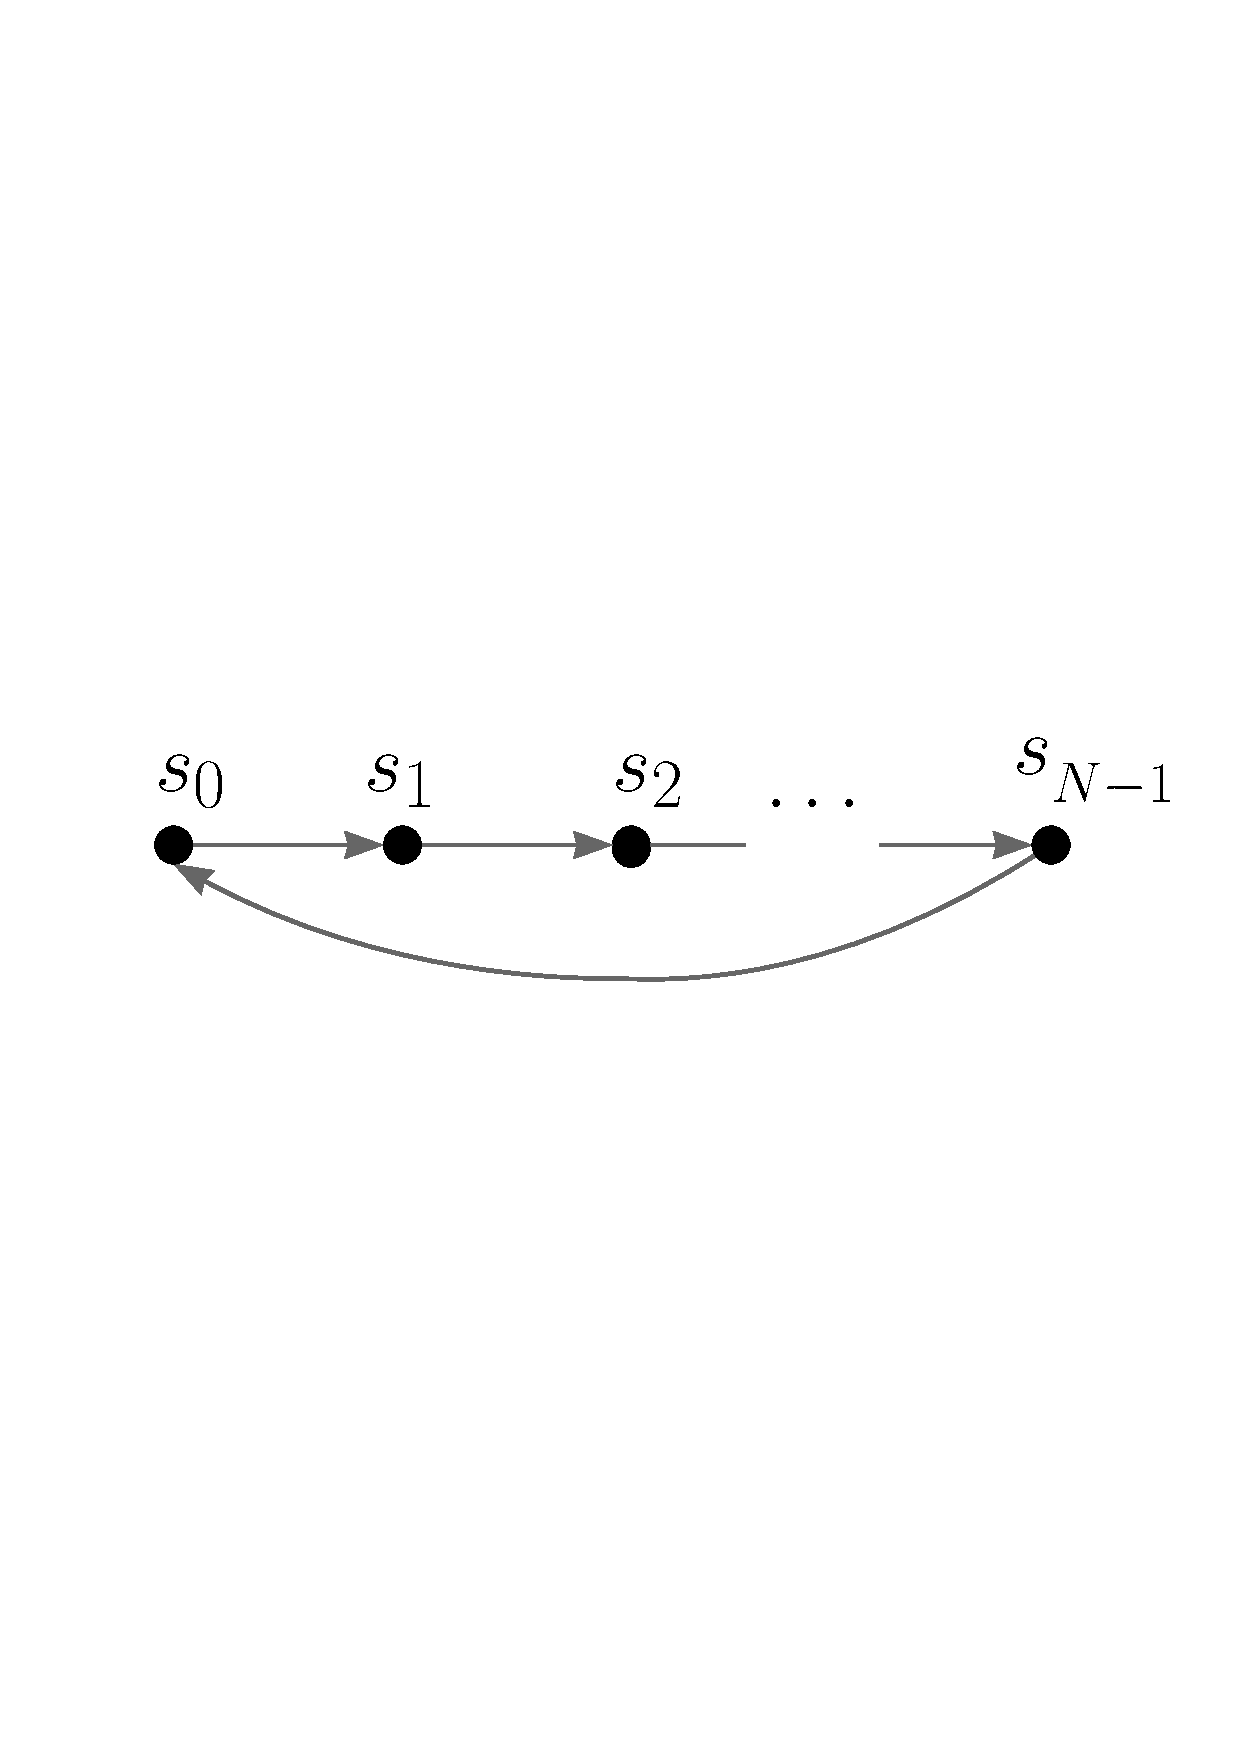
\includegraphics[width=0.25\linewidth]{Figures/signal_ring_graph_white_border.pdf}
	}
	\subfloat[\label{figb_graphs}]{
		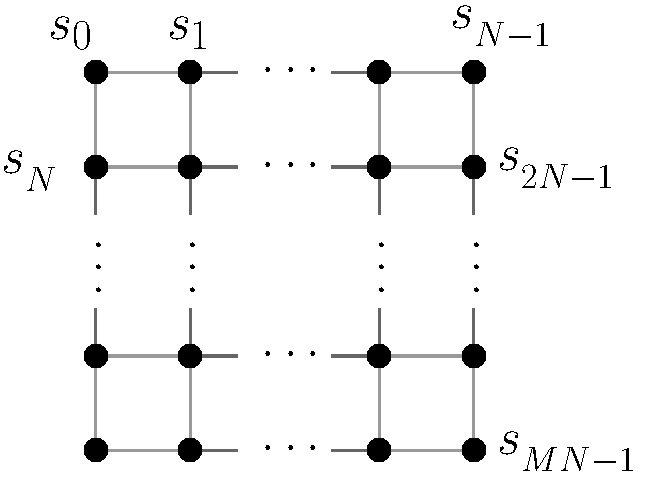
\includegraphics[width=0.25\linewidth]{Figures/image_graph.pdf}
	}%
	\subfloat[\label{figd_graphs}]{
		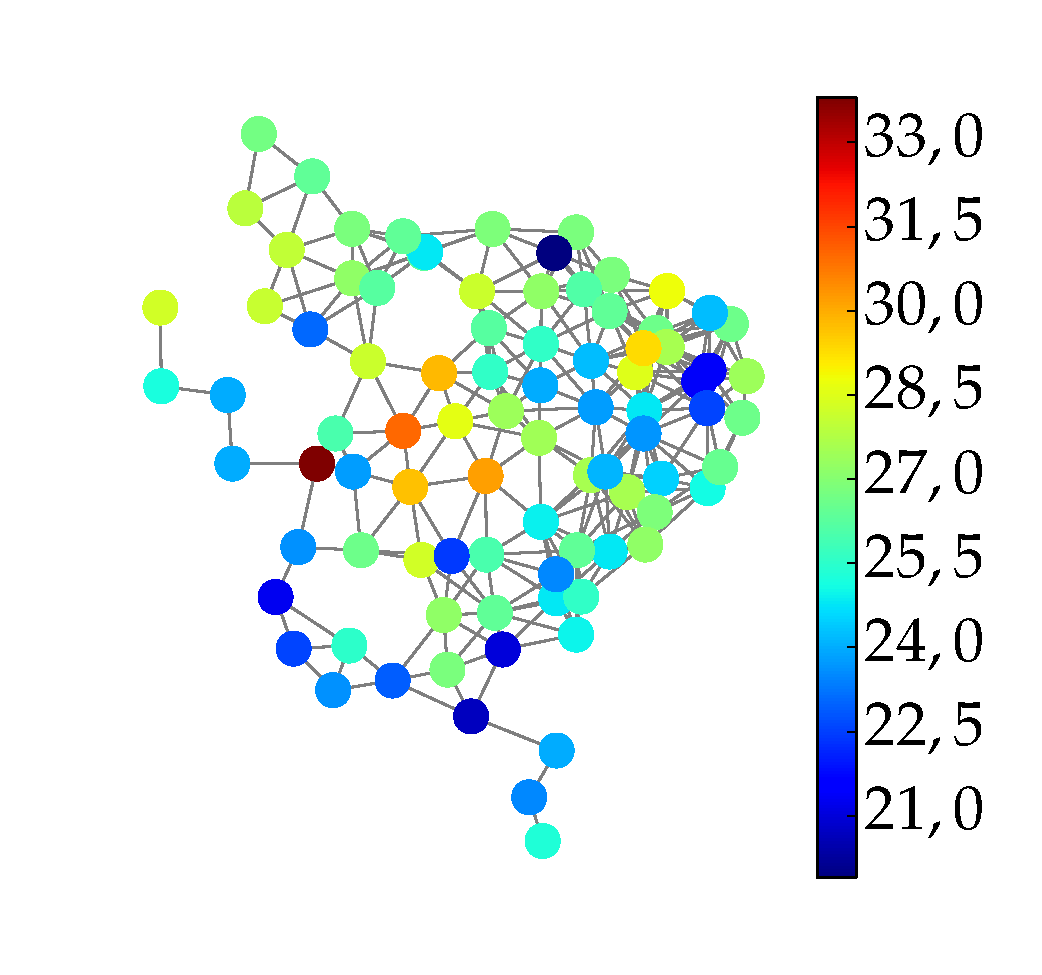
\includegraphics[width=0.26\linewidth]{Figures/temp_NE_stretched.pdf} }%
	\caption{Representa\c{c}\~oes de sinais sobre (a) um grafo em anel direcionado, (b) um grafo em grade retangular uniforme  e (c) um grafo formado por cidades do Nordeste brasileiro.}%
	\label{fig:graphs}%
	%	\vspace{-0.9cm}
	%	{\\ \small Fonte: o autor.}
\end{figure}

Um sinal de comprimento finito e de tempo discreto \'e modelado pelo grafo em anel direcionado (considera-se os pesos unit\'arios), como mostrado na Fig.~\ref{figa_graphs}: a no\c c\~ao de evolu\c c\~ao temporal \'e capturada pelas arestas direcionadas; a periodicidade imposta pelas condi\c c\~oes de fronteira da an\'alise de Fourier de tempo discreto \'e modelada pela aresta realimentando a \'ultima amostra \`a primeira. O grafo na Fig. \ref{figb_graphs} \'e um modelo para imagens digitais \cite{sandryhaila2012nearest} chamado \emph{nearest-neighbor}, em que a depend\^encia entre pixels \'e aproximada para existir apenas entre vizinhos, e o grafo na Fig. \ref{figd_graphs} \'e um exemplo de grafo de rede de sensores\footnote{Quando n\~ao \'e especificado em contr\'ario, chama-se \emph{grafo de (rede de) sensores} um grafo conectado com v\'ertices distribu\'idos uniformemente numa regi\~ao do espa\c co euclidiano bidimensional.}, com pesos das arestas dados pelo inverso da dist\^ancia euclidiana, sobre o qual definiu-se o sinal da temperatura \`a meia-noite de 01 de fevereiro de 2012 em cidades do Nordeste brasileiro\footnote{Fonte: Banco de Dados Meteorol\'ogicos para Ensino e Pesquisa (BDMEP) do Instituto Nacional de Meteorologia. Acesso gratuito, dispon\'ivel em: \url{http://www.inmet.gov.br/portal/index.php?r=bdmep/bdmep}}.

As caracter\'isticas espectrais de um sinal dependem fortemente do dom\'inio sobre o qual ele \'e definido. %, mas n\~ao faz sentido reconhecer essa depend\^encia em Processamento Cl\'assico de Sinais porque nele trabalha-se apenas com dom\'inios regulares e uniformes\footnote{Mesmo quando se aborda \emph{amostragem n\~ao-uniforme}, as t\'ecnicas desenvolvidas ainda visam \`a \emph{recupera\c{c}\~ao} do sinal em um dom\'inio -- de tempo -- tipicamente regular.}.
Em geral, diz-se que um sinal cont\'em majoritariamente baixas frequ\^encias se amostras \emph{adjacentes} t\^em valores \emph{pr\'oximos}, e altas frequ\^encias se t\^em valores \emph{d\'ispares}. Considerando sinais definidos sobre grafos, fica evidente que a no\c c\~ao de amostras adjacentes depende da topologia do grafo em quest\~ao, e portanto \emph{um mesmo sinal pode apresentar espectros distintos se definido sobre grafos diferentes}. 
%A Fig. \ref{fig:diff_struct} confirma essa intui\c c\~ao, apresentando o espectro de um sinal segundo a base de autovetores da matriz Laplaciana do grafo, para dois grafos distintos; na Fig. \ref{fig:diff_struct_b}, as amostras de maior valor s\~ao adjacentes \`aquelas de menor valor, o que causa componentes de maior frequ\^encia do que se o grafo usado como dom\'inio fosse um anel a pesos constantes (Fig. \ref{fig:diff_struct_a}).

%Em 2006, P\"uschel e Moura publicaram sua teoria de processamento alg\'ebrico de sinais (ASP, do ingl\^es \emph{algebraic signal processing}) \cite{moura2006algebraic}. A descrição de sinais e filtros do ponto de vista alg\'ebrico \'e intencionalmente abstrata e gen\'erica: tanto os filtros como os sinais s\~ao simplesmente elementos de espa\c cos vetoriais dotados de multiplica\c c\~ao e distributividade. Especificamente, o espa\c co de filtros \'e uma \emph{\'algebra}, sobre a qual toma-se um \emph{m\'odulo} para ser o espa\c co de sinais. Uma descri\c c\~ao detalhada sobre ASP foge ao escopo deste cap\'itulo, mas o leitor interessado pode tirar bastante proveito dos trabalhos originais de P\"uschel e Moura \cite{puschel2008time,puschel2008space}.
%
%O aspecto de ASP que levou ao processamento sobre grafos, o que de fato nos interessa diretamente, \'e que o espa\c co de filtros \'e \emph{gerado} pelo operador de atraso unit\'ario de sinais. Um exemplo tornar\'a a afirma\c c\~ao menos obscura: seja a \'algebra polinomial $ \mathbb{C}[x] / (x^N - 1) $, ou $ {A}  = \{ \sum_{\ell=0}^{N-1} a_\ell x^\ell | a_\ell \in \mathbb{C} \}$, que consiste em todos os polin\^omios de coeficientes complexos com grau menor do que $ N $, dotados da adi\c c\~ao e multiplica\c c\~ao polinomiais usuais, m\'odulo $ x^N - 1 $. \'E comum representar sinais e filtros de tempo discreto e comprimento $ N $ como elementos de $ {A}  $, caso em que a convolu\c c\~ao c\'iclica torna-se a simples multiplica\c c\~ao polinomial modular. Por exemplo, o sinal $ \mathbf{s}_1 = (0 \ \ 2 \ \ 1 \ \ 0) $ \'e representado por $ s_1(x) = x^2 + 2x $, e sua vers\~ao deslocada de uma unidade, $ \mathbf{s}_2 = (0 \ \ 0 \ \ 2 \ \ 1) $, \'e dada por $ s_2(x) = x^3 + 2x^2 $. Fica claro que, neste caso, o filtro de atraso unit\'ario \'e $ d(x) = x $, cujas pot\^encias \emph{geram} a base $ (1, x, x^2, \dots, x^{N-1}) $ para o espa\c co de filtros. Esta rela\c c\~ao se mant\'em para qualquer \'algebra em ASP; portanto, Moura certamente concluiu que, ao definir um operador de deslocamento unit\'ario para sinais sobre grafos, isto daria in\'icio \`a constru\c c\~ao da teoria de GSP.

Um conceito fundamental em GSP \'e o de operador de deslocamento. Trata-se de uma matriz quadrada $ S $ extra\'ida a partir do grafo $ \mathcal{G} $, tal que $ S_{ji} $ somente pode ser n\~ao-nulo se $ i = j $ ou $ (v_i, v_j) $ for uma aresta de peso n\~ao-nulo de $ \mathcal{G} $ \cite{segarra2015interpolation}. Escolhas usuais para $ S $ s\~ao a matriz de adjac\^encia \cite{sandryhaila2014big} e a Laplaciana \cite{shuman2013emerging}, embora outras op\c c\~oes existam (e.g. \cite{girault2015translation, dees2019unitary}), a depender de qual propriedade se deseje. O restante da se\c c\~ao tomar\'a a matriz de adjac\^encia como operador de deslocamento, por ser aquele que mais claramente transmite a no\c c\~ao de atraso unit\'ario do sinal no grafo. Pode-se ver que a multiplica\c c\~ao de um sinal $ \mathbf{x} $ \`a esquerda por $ \mathbf{A} $ faz com que cada amostra $ x_i $ seja redistribu\'ida para os v\'ertices vizinhos, ponderada pelo peso das arestas que saem do v\'ertice $ i $:
\begin{equation}
y_j = \sum_{i=0}^{N-1} A_{ij} x_i.
\end{equation}

O conceito fica ainda mais claro ao se tomar o grafo em anel direcionado com pesos unit\'arios, modelo para o dom\'inio de tempo discreto (Fig. \ref{figa_graphs}). Pode-se ver que sua matriz de adjac\^encia,
\begin{equation}\label{eq:C}
\mathbf{C} =
\left[\renewcommand{\arraystretch}{0.65}\begin{array}{cccc}
&  &  &   1\\ 
1 &  &   & \\ 
&   \ddots &  & \\ 
&  &   1 & 
\end{array}\right],
\end{equation}
\noindent realiza precisamente o papel de atraso num sinal de tempo discreto. Ou seja, se um sinal $ \mathbf{s} = (s_1 \ s_2 \ \dots \ s_N)^T $ definido em um grafo em anel \'e multiplicado \`a  esquerda por $ \mathbf{C} $, tem-se
\begin{equation}\label{eq:graph_shift_C}
\mathbf{s}^{\langle 1 \rangle} = \mathbf{C} \mathbf{s},
\end{equation}
com $ \mathbf{s}^{\langle 1 \rangle} = (s_N \ s_1 \ \dots \ s_{N-1})^T $.
Para um sinal $ \mathbf{x} $ sobre um grafo qualquer $ \mathcal{G} = \{\mathcal{V}, \mathbf{A}\} $, $ \mathbf{A} $ age como um \emph{filtro} de atraso (ou deslocamento) sobre $ \mathbf{x} $, e a vers\~ao deslocada deste sinal \'e representada por $ \mathbf{x}^{\langle 1 \rangle} = \mathbf{A} \mathbf{x}$.

%e a opera\c c\~ao de deslocamento do sinal,
%\begin{equation}
%%\label{key}
%\widetilde{\mathbf{x}} = \mathbf{A} \mathbf{x} \Rightarrow \widetilde{x}_i = \sum_{j=0}^{N-1} A_{i,j} x_j,
%\end{equation}
%significa substituir o valor em cada v\'ertice do grafo pela soma dos valores adjacentes, ponderada pelos pesos das arestas incidentes. No dom\'inio do tempo discreto, o deslocamento \'e a mera transfer\^encia c\'iclica de valor das amostras porque o grafo subjacente \'e em anel a pesos constantes (Fig. \ref{figa_graphs}).

\subsection{Filtros sobre grafos}
\label{subsec:filtros}

Observar a matriz de adjac\^encia como um filtro levou \`a defini\c c\~ao de um filtro de sinais sobre grafos como sendo qualquer matriz $ \mathbf{H} \in \mathbb{C}^{N \times N} $ \cite{sandryhaila2013filters}, visto que o produto matriz-vetor sempre resulta num vetor (ou \emph{filtro} $ \times $ \emph{sinal} $ = $ \emph{sinal}). Isso implica que os filtros sobre grafos s\~ao sempre lineares, uma vez que a distributividade da multiplica\c c\~ao em rela\c c\~ao \`a adi\c c\~ao matricial garante que
\begin{equation}
%\label{key}
\mathbf{H} (\alpha_1 \mathbf{x}_1 + \alpha_2 \mathbf{x}_2) =  \alpha_1 \mathbf{H} \mathbf{x}_1 + \alpha_2 \mathbf{H}  \mathbf{x}_2.
\end{equation}

A propriedade de invari\^ancia no tempo (ou ao deslocamento) requer que $ \mathbf{A} \mathbf{H} \mathbf{x} = \mathbf{H} \mathbf{A} \mathbf{x} {,} \ \forall \mathbf{x}$. Uma classe de filtros que sempre obedece a esse requisito s\~ao aqueles na forma de um polin\^omio $ h(\cdot) $ avaliado em $ \mathbf{A} $,
\begin{equation}
\label{eq:filter_poly}
h(\mathbf{A}) = \sum_{\ell=0}^{L-1} h_\ell \mathbf{A}^\ell,
\end{equation}
com $ L$ menor ou igual ao grau do polin\^omio m\'inimo $ m_\mathbf{A} $ de $ \mathbf{A}$~\cite{sandryhaila2013discrete,sandryhaila2014big}. Assim, estes filtros LSI s\~ao uma s\'erie de pot\^encias finita no operador de deslocamento, exatamente como ocorre em processamento cl\'assico de sinais de tempo discreto, em que os filtros LTI t\^em representa\c c\~ao em termos de polin\^omios em $ z^{-1} $, pela transformada Z. A menos que dito em contr\'ario, ser\'a utilizado o termo ``filtro LSI`` como sin\^onimo para um filtro como (\ref{eq:filter_poly}).

\subsection{A transformada de Fourier sobre grafos}

Uma vez que a transformada de Fourier de um sinal \'e a sua proje\c{c}\~ao em uma base de fun\c{c}\~oes invariantes \`a  filtragem linear e invariante no tempo (LTI, do ingl\^es \emph{linear and time-invariant}) \cite{oppenheim1997signals}, em GSP define-se a transformada de Fourier sobre grafos (GFT, do ingl\^es \emph{graph Fourier transform}) como a decomposi\c{c}\~ao de um sinal em termos de uma base de autovetores do operador de deslocamento --- e, portanto, autovetores da filtragem LSI~\cite{sandryhaila2013gft}.

Seja $ \mathbf{A} $ a matriz de adjac\^encia de um grafo de $ N $ v\'ertices. Se $ \mathbf{A} $ for diagonaliz\'avel, tem-se\footnote{Se $\mathbf{A}$ n\~ao for diagonaliz\'avel, o racioc\'inio pode ser repetido utilizando-se a forma can\^onica de Jordan.}
\begin{equation}\label{eq:gft_01}
\mathbf{A} = \mathbf{V} \mathbf{\Lambda} \mathbf{V}^{-1},
\end{equation}
em que $ \mathbf{V} $ cont\'em os $ N $ autovetores de $ \mathbf{A} $ em suas colunas, isto \'e,
\begin{equation}\label{eq:gft_02}
\mathbf{V} = (\mathbf{v}_0 \ \mathbf{v}_1 \ \dots\ \mathbf{v}_{N-1}).
\end{equation}

Como filtros LSI s\~ao polin\^omios em $ \mathbf{A} $, as colunas de $ \mathbf{V} $ formam uma base de vetores invariantes \`a  filtragem LSI
%. Somando a isto o fato de que os subespa\c{c}os gerados pelos autovetores de um mesmo autovalor de $ \mathbf{A} $ s\~ao irredut\'iveis, t\^em interse\c{c}\~ao nula e suas dimens\~oes somam $ N $ \cite{sandryhaila2013gft}, $ \mathbf{V} $ fornece uma base invariante \`a  filtragem LSI
para o espa\c{c}o de sinais $ \mathcal{S} $ sobre o grafo com matriz de adjac\^encia $ \mathbf{A} $. Desta forma, um sinal $ \mathbf{x} \in \mathcal{S} $ pode ser decomposto em suas componentes na base $ \mathbf{V} $ como
\begin{align}\label{eq:GFT_inv}
\mathbf{x} &= \widehat{x}_0 \mathbf{v}_0 + \dots + \widehat{x}_{N-1} \mathbf{v}_{N-1} = \mathbf{V} (\widehat{x}_0 \ \widehat{x}_1 \ \dots \ \widehat{x}_{N-1})^T \notag \\
&= \mathbf{V} \widehat{\mathbf{x}},
\end{align}
e esta \'e definida como a equa\c{c}\~ao de s\'intese da \emph{transformada de Fourier sobre grafos}. A equa\c{c}\~ao de an\'alise da GFT \'e, portanto,
\begin{equation}\label{eq:GFT_fwd}
\widehat{\mathbf{x}} = \mathbf{V}^{-1} \mathbf{x}.
\end{equation}

Para sinais de tempo discreto, foi assinalado que seu dom\'inio \'e modelado como um grafo com matriz de adjac\^encia $ \mathbf{C} $ em~(\ref{eq:C}). Como $ \mathbf{C} $ \'e circulante, ela \'e diagonalizada pela matriz da transformada discreta de Fourier (DFT, do ingl\^es \emph{discrete Fourier transform}), dada por $ \mathbf{F} $, $ F_{n,k} = \exp \left( -\jmath\frac{2 \pi}{N} nk \right) $. Assim, pode-se escrever%, que cont\'em em suas linhas os autovetores da DFT. Atrav\'es do polin\^omio caracter\'istico de $ \mathbf{C} $,
%\begin{equation}
%\label{key}
%p_{\mathbf{C}}(\lambda) = \text{det} (\lambda \mathbf{I} - \mathbf{C}) =
%\begin{vmatrix}
%\lambda &  &  &   -1\\ 
%-1 & \lambda &   & \\ 
%&   \ddots & \ddots & \\ 
%&  &   -1 & \lambda
%\end{vmatrix}
%=\lambda^N - 1,
%\end{equation}
%mostra-se que seus autovalores s\~ao as $ N $ ra\'izes da unidade. Assim, a diagonaliza\c c\~ao da matriz $ \mathbf{C} $ pela matriz da DFT \'e escrita como
\begin{equation}\label{eq:diag_C}
\mathbf{C} = \mathbf{F}^{-1} \mathbf{\Lambda}_{\mathbf{C}} \mathbf{F},
\end{equation}
em que $\mathbf{\Lambda}_{\mathbf{C}}$ \'e uma matriz diagonal com os autovalores de $\mathbf{C}$. V\^e-se que a matriz da GFT, para grafos em anel, \'e $ \mathbf{V}^{-1} = \mathbf{F} $, o que resulta na desej\'avel propriedade de que a GFT de sinais de tempo discreto coincide com a  DFT, demonstrando consist\^encia com a teoria cl\'assica.

\subsection{O dom\'inio da frequ\^encia}

A defini\c c\~ao empregada para a GFT sugere interpretar os autovetores $ \mathbf{v}_i $ da matriz de adjac\^encia como as ``componentes de frequ\^encia'' associadas \`as \emph{frequ\^encias de grafo} representadas pelos autovalores $ \lambda_i $ (como a componente de Fourier $ {\text{e}}^{-\jmath \Omega t} $, no dom\'inio do tempo cont\'inuo $ t $, \'e associada \`a frequ\^encia $ \Omega $). A menos que os polin\^omios caracter\'istico e m\'inimo de $ \mathbf{A} $ sejam iguais, uma mesma frequ\^encia estar\'a associada a duas ou mais componentes linearmente independentes, como ocorreu com o sinal na Fig. \ref{fig:diff_struct_GSPA}. Na mesma figura, nota-se que, embora o sinal seja visualmente suave, seu espectro possui componentes associadas a autovalores de grande magnitude, o que levanta a quest\~ao de definir um crit\'erio coerente para se falar em \emph{altas} e \emph{baixas} frequ\^encias de sinais sobre grafos.


\begin{figure}
\centering
\begin{minipage}[c]{0.3\linewidth}
	\subfloat[\label{fig:diff_struct_a_GSPA}]{
		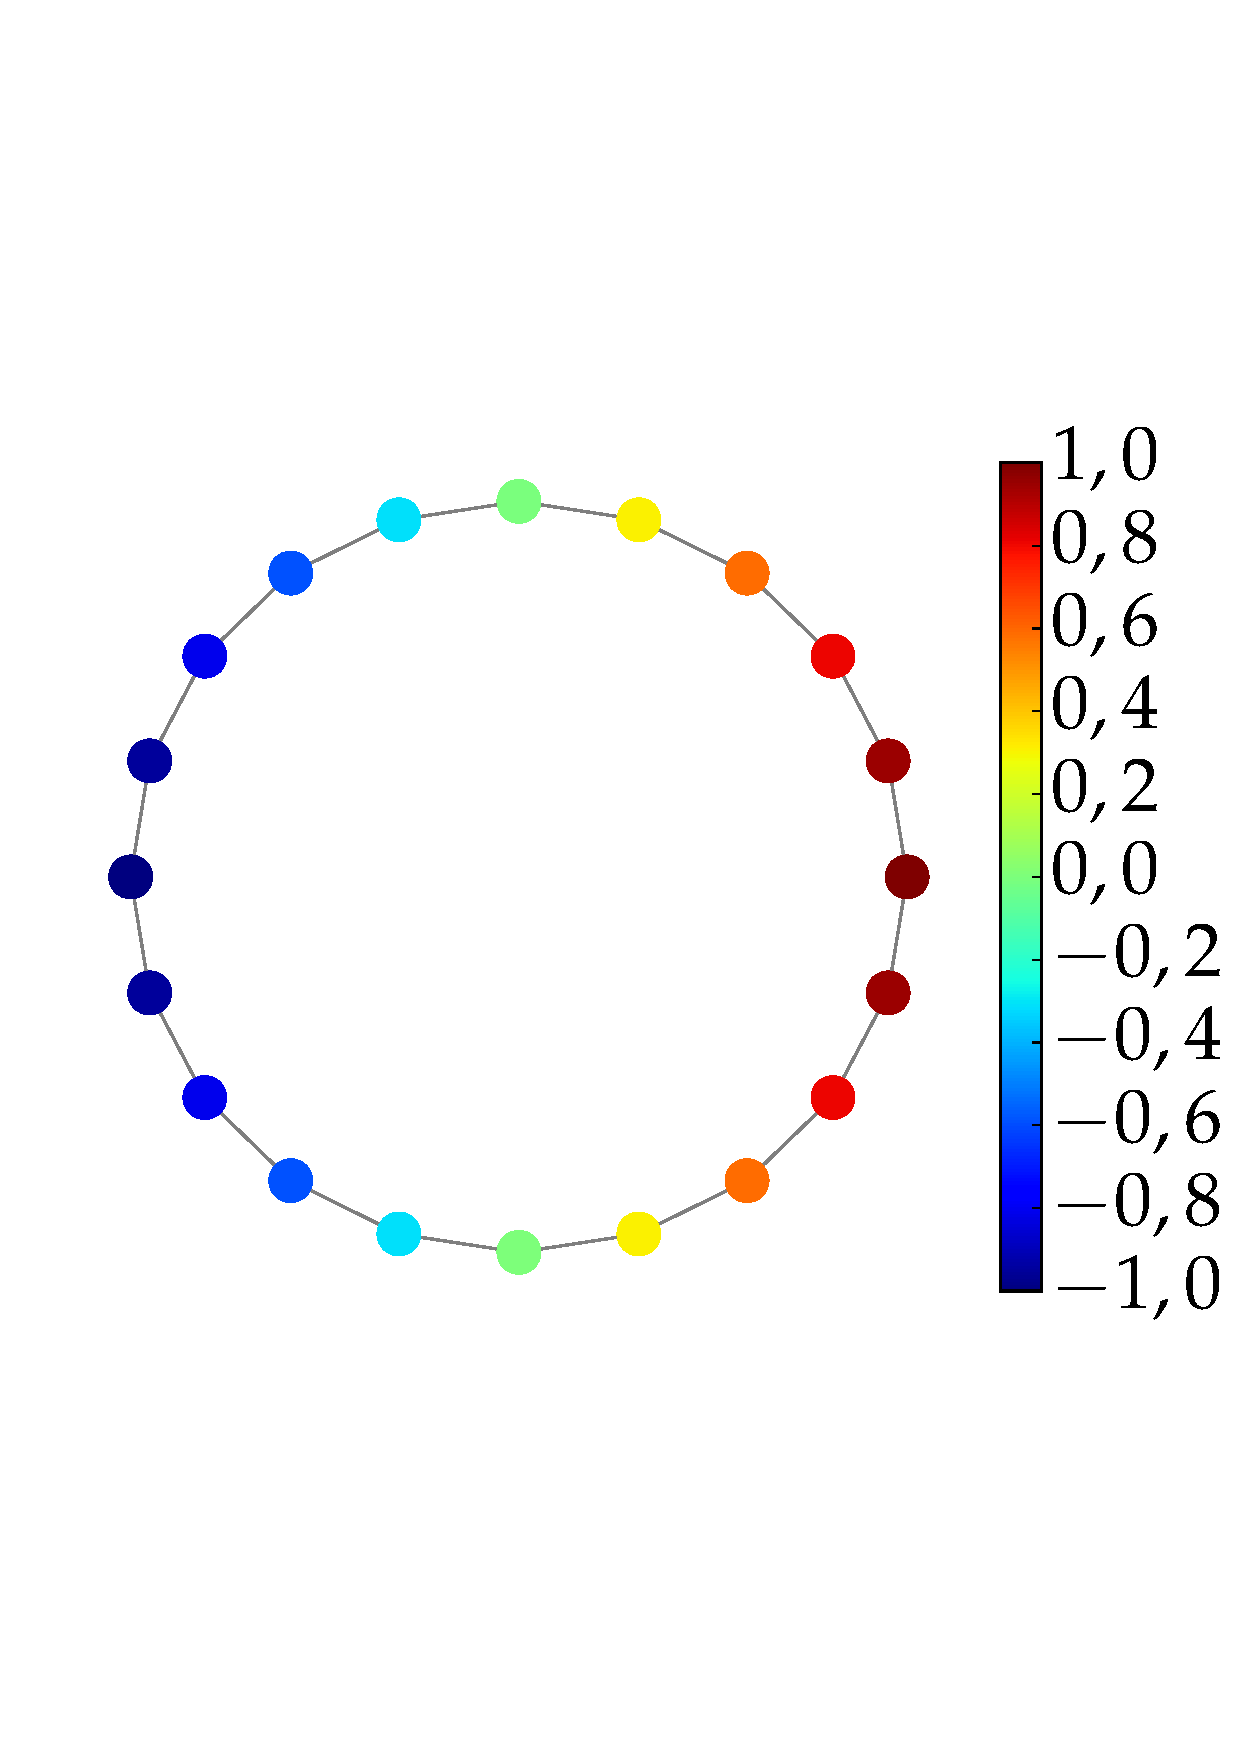
\includegraphics[width=\linewidth]{Figures/ring_different_structure_01_GSPA_larger.pdf}
	}
\end{minipage} %
\begin{minipage}[c]{0.27\linewidth}
	\subfloat[\label{fig:diff_struct_b_GSPA}]{
		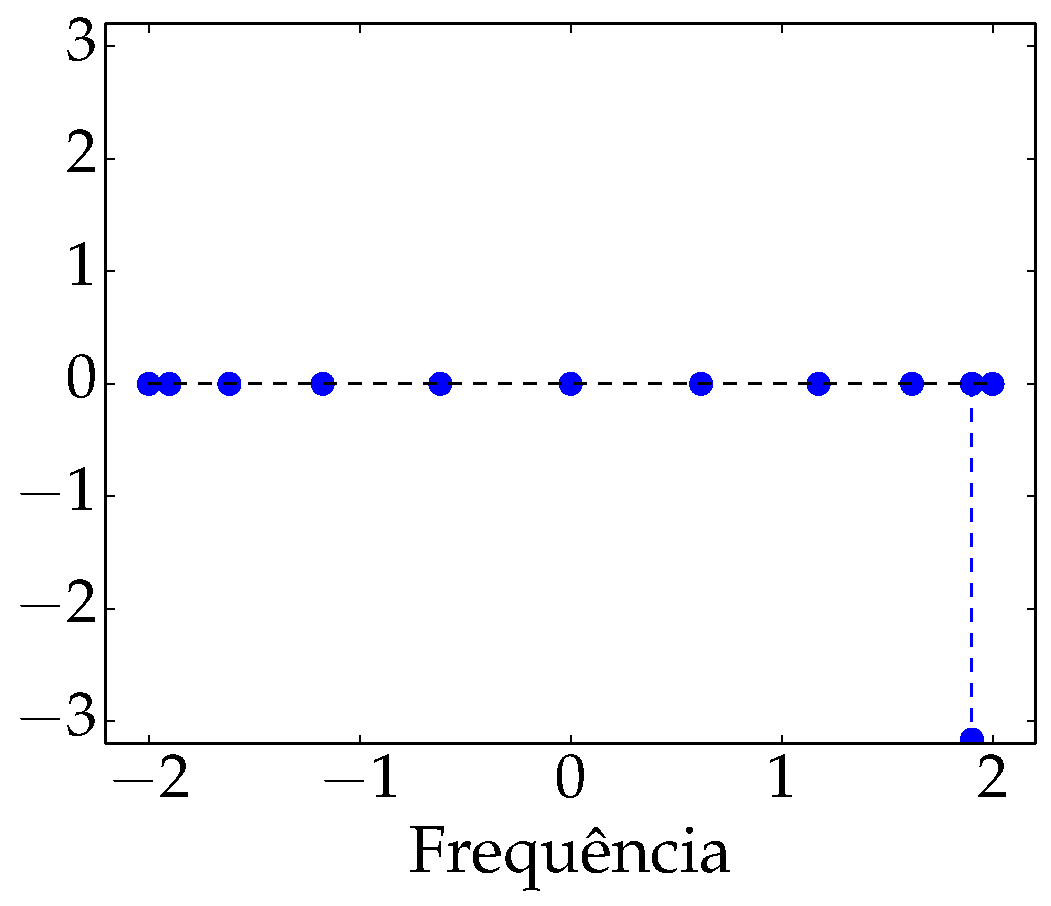
\includegraphics[width=\linewidth]{Figures/ring_different_structure_01_spectrum_GSPA_PT_2.pdf}
	}
\end{minipage}%
\caption{(a) Sinal sobre um grafo em anel n\~ao-direcionado e (b) seu espectro em GSP\textsubscript{A}.}%
\label{fig:diff_struct_GSPA}%
%	\vspace{-0.2cm}
%	{\\ \small Fonte: o autor.}
\end{figure}

Para fundamentar matematicamente a no\c c\~ao de frequ\^encia no contexto de GSP, partiu-se de uma m\'etrica usual para sinais de tempo discreto: a \emph{varia\c c\~ao total}, que calcula a soma das diferen\c cas entre amostras adjacentes de um sinal e, portanto, assume valores maiores para sinais de maior frequ\^encia. Sua express\~ao matem\'atica, para certo sinal de comprimento finito $ \mathbf{x} = (x_0 \ \ x_1 \ \ \dots \ \ x_{N-1}) $, \'e
\begin{equation}
\label{eq:TV}
TV(\mathbf{x}) = \sum_{n=0}^{N-1} | x_n - x_{n-1 \text{ mod } N}|.
\end{equation}

De (\ref{eq:C}) e (\ref{eq:graph_shift_C}), v\^e-se que (\ref{eq:TV}) pode ser reescrita em termos da norma $ \ell_1 $\footnote{A norma $ \ell_1 $ \'e um caso particular da norma $ \ell_p $ de um vetor $ \mathbf{x} \in \mathbb{C}^{N} $, definida como $ \Vert \mathbf{x}\Vert_p \overset{\Delta}{=} \left(\sum_{k=0}^{N-1} |x_k|^p\right)^{1/p} $. Quando n\~ao for explicitamente indicado, a nota\c c\~ao sem subscrito $ \Vert \cdot \Vert $ indica a norma $ \ell_2 $.} como $ TV(\mathbf{x}) = \Vert \mathbf{x} - \mathbf{C x}\Vert_1 $, utilizando a matriz de adjac\^encia do grafo em anel para realizar o deslocamento c\'iclico do sinal. Assim, uma generaliza\c{c}\~ao da fun\c c\~ao $ TV(\cdot) $ para sinais definidos sobre grafos quaisquer, i.~e., a \emph{varia\c c\~ao total sobre grafos} para um sinal $ \mathbf{s} $ sobre o grafo $ \mathcal{G} = \{\mathcal{V}, \mathbf{A}\} $, foi definida como
\begin{equation}
\label{eq:var_total}
TV_G(\mathbf{s}) \overset{\Delta}{=} \Vert \mathbf{s} - \mathbf{A}^{\text{\emph{norm}}} \mathbf{s}\Vert_1,
\end{equation}
com $ \mathbf{A}^{\text{\emph{norm}}} = |\lambda_{max}|^{-1}\mathbf{A} $ e $ \lambda_{max} $ o autovalor de $ \mathbf{A} $ com maior m\'odulo. A normaliza\c c\~ao de $ \mathbf{A} $ visa evitar a magnifica\c c\~ao excessiva das amostras do sinal deslocado \cite{sandryhaila2014frequency}.

\begin{figure}
	\centering
	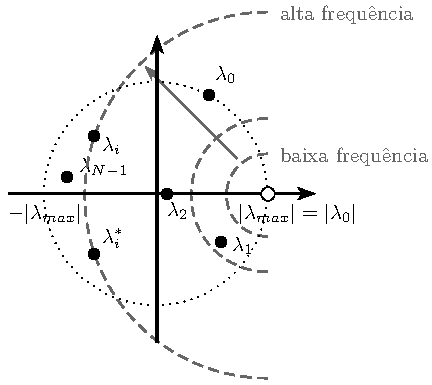
\includegraphics[width=0.35\linewidth]{Figures/graph_frequency.pdf}
	\caption{Ordenamento das frequ\^encias de sinais sobre grafos, de baixa para alta, no plano complexo. Fonte: adaptado de \cite{sandryhaila2014frequency}.}
	\label{fig:ordem_freq}
	%	{\\ \small Fonte: adaptado de \cite{sandryhaila2014frequency}.}
\end{figure}

Seja $ \mathbf{A} $ diagonaliz\'avel e com autovalores (possivelmente complexos) ordenados tais que
\begin{equation}
\label{eq:eig_order}
|\lambda_0| \leq |\lambda_1| \leq \dots \leq |\lambda_{N-1}| \overset{\Delta}{=} |\lambda_{max}|,
\end{equation}
associados aos autovetores $ (\mathbf{v}_i)_{i=0,\dots,N-1} $ escolhidos de modo que $ \Vert \mathbf{v}_k \Vert_1 = 1 $. Tomando a varia\c c\~ao total de um autovetor $ \mathbf{v}_k $ associado a $ \lambda_k $, tem-se
\begin{align*}
%\label{key}
TV_G(\mathbf{v}_k) &= \Vert \mathbf{v}_k - \mathbf{A} \mathbf{v}_k \Vert_1  = \Vert\mathbf{v}_k - \frac{1}{|\lambda_{max}|} \lambda_k \mathbf{v}_k \Vert_1 = \left|1 - \frac{\lambda_k}{|\lambda_{max}|}\right| \Vert \mathbf{v}_k \Vert_1 = \Big| \lambda_k - |\lambda_{max}| \Big| \frac{\Vert \mathbf{v}_k \Vert_{1}}{|\lambda_{max}|}
\end{align*}
de forma que, como foi feito $ \Vert \mathbf{v}_k \Vert_1 = 1 $, tem-se a equival\^encia
\begin{equation}
\label{eq:TV_ordering}
\Big|  \lambda_i - |\lambda_{max}|\Big| \leq \Big|  \lambda_j - |\lambda_{max}|\Big| \iff TV_G(\mathbf{v}_i) \leq TV_G(\mathbf{v}_j),
\end{equation}
ou seja, componentes de frequ\^encia associadas a autovalores mais pr\'oximos do ponto $ |\lambda_{max}| $ no plano complexo s\~ao mais suaves e s\~ao, portanto, ditas de \emph{baixa frequ\^encia}. A Fig. \ref{fig:ordem_freq} ilustra esse ordenamento para as frequ\^encias de grafos, o que esclarece a leitura do espectro do sinal na Fig. \ref{fig:diff_struct_a_GSPA}, cuja matriz de adjac\^encia tem autovalores reais.


\chapter{The fractional graph shift operator and its applications}

Over the last decade, theory and applications related to graph signal processing (GSP) have been widely developed and attracted the attention of several scholars~\cite{ortega2018,richard2018,ribeiro2018}. In short, GSP aims to extend concepts and operations of classical digital signal processing (DSP) to scenarios in which the signals lie over irregular domains. Such scenarios include, for instance, sensors arbitrarily positioned in a geographic region and measuring some climatological variable, points of a three-dimensional cloud representing some virtual object and its attributes, people linked according to their interests and proximity relationships in a social network and so on~\cite{chen2014,zhang2014,benzi2016,weiyu2018,saad2018,jiang2021,gama2019,liu2019,zhang2020,ferreira2020,zhang2021,xiao2021,sun2021}. To be more specific, among the issues related to the referred scenarios, one can cite segmentation and attribute compression of 3D point clouds~\cite{zhang2014,zhang2020}, stochastic filtering under asymmetric links in wireless sensor networks~\cite{saad2018}, community detection in social networks~\cite{zhang2021}, anomalous IoT sensor data detection~\cite{xiao2021} and traffic prediction via attention networks~\cite{sun2021}. It is intuitive that the mentioned examples can be modeled as graphs whose vertices are connected by edges inferred from a variety of influence or dependency criteria. This contrasts with the discrete-time domain, over which the samples of a signal are equidistantly placed and have left- and right-side immediate neighbors only; something similar happens in the case of digital images, where the pixels are arranged in a regular rectangular grid.

Two main GSP approaches have been consolidated throughout the last years. The first is based on the spectral graph theory and analyzes signals on undirected graphs with real and non-negative edge weights, by using the graph Laplacian to construct a basis for the signal space~\cite{shuman2013emerging}. The second comes from the algebraic signal processing and uses the weighted adjacency matrix $\mathbf{A}$ as elementary building block~\cite{puschel2008time,puschel2008space}; such an approach, which is adopted in this paper, allows to deal with signals defined over both directed and undirected graphs, and with real- and complex-valued edge weights~\cite{sandryhaila2014big}. \textcolor{black}{In any case, the aforementioned approaches have used $\mathbf{L}$ and $\mathbf{A}$ as elementary building blocks because, among other reasons, these matrices are well established in graph theory and allow some meaningful physical interpretation or some parallel with the classical DSP; while $\mathbf{A}$ can be viewed as a generalization of the discrete-time unit shift, $\mathbf{L}$ is a kind of discrete counterpart to the continuous Laplace-Beltrami (second order) derivative operator on a manifold~\cite{chung1997spectral,Coifman2005}.}

Among the research fronts active in GSP, the one that investigates alternatives to the operators usually employed as building blocks to describe graph signals and systems deserves to be highlighted~\cite{girault2015translation,gavili2017,fan20191,fan2019,mollaebrahim2021,shafipour2018,shafipour2019}. \textcolor{black}{In fact, when the purpose is to consider linear operators in this context, any matrix can be chosen to play the role of elementary building block; multiplying a matrix by a graph signal represented as a vector produces another signal whose samples result from a linear combination of the samples of the original signal. In this scope,} the use of matrices other than the \textit{standard} adjacency matrix and the Laplacian for the mentioned purpose may \textcolor{black}{be more suitable in specific scenarios and to carry out specific (graph) signal processing tasks. Even when the focus is on designing other graph operators (e.g., the graph Fourier transform), the decision about which elementary operator to use has an impact on the expected results.}

\textcolor{black}{Regarding the issue discussed in the last paragraph, some works archived in the GSP literature can be brought to the fore. In~\cite{girault2015translation}, for example, the authors propose an isometric graph translation operator that is described in the spectral domain as a phase shifting operator; this operator shares key properties with the time shift and behaves reasonably in the vertex domain. In~\cite{gavili2017}, the authors define an energy-preserving shift operator that satisfy many properties similar to their counterparts in classical signal processing; the GSP framework based on the referred operator enables the signal analysis along a correlation structure defined by a graph shift manifold. In~\cite{fan20191} and~\cite{fan2019}, the authors employ different features associated with a graph to generate a series of shift operators and design a graph-filter-based classifier. Although the proposed method produces better results than those achieved using conventional graph-filter-based classifiers, it requires dealing with a non-convex optimization problem whose solution involves a relatively high computational cost. In~\cite{mollaebrahim2021}, motivated by the typical scenario of asymmetric communications in wireless sensor networks, the authors study the optimal design of graph shift operators to perform decentralized subspace projection for asymmetric topologies. Obtaining the referred operators can be performed either by solving an optimization problem or by employing a decentralized algorithm based on an Alternating Direction Method of Multipliers (ADMM). In~\cite{shafipour2018} and~\cite{shafipour2019}, the goal is to construct a graph Fourier transform for directed graphs (digraphs), such that the corresponding orthonormal frequency components are as spread as possible in the graph spectral domain. The method uses the Laplacian of an undirected version of the digraph and involves non-convex, orthonormality-constrained optimization problems.} 

\textcolor{black}{This paper is somehow related to the above mentioned works, since its central theme refers to elementary operators on graphs. To be more specific, we consider the} possibility of \textcolor{black}{computing} a non-integer power $\mathbf{A}^a$, $a\in\mathbb{R}$, of the adjacency matrix $\mathbf{A}$, \textcolor{black}{which is taken as} the (unit) graph shift operator~\cite{sandryhaila2014big}. \textcolor{black}{With this,} we introduce the notion of fractional shift (or delay) of signals on graphs, \textcolor{black}{which, to the best of our knowledge, has not yet been addressed in the literature. Differently from the referred papers, in which new operators are created or standard operators are adjusted using strategies potentially expensive from the computational point of view, we propose a relatively simple generalization that fills a theoretical gap concerning the extension to the GSP framework of a well-established concept in the classical signal processing.}

\color{black}
In what follows, the main contributions of this paper are listed:
\begin{itemize}
\item We introduce the fractional graph shift operator $\mathbf{A}^a$ and discuss its several aspects. More specifically, we demonstrate that $\mathbf{A}^a$ can be computed by using the theory of matrix functions, considering the Jordan decomposition of $\mathbf{A}$.
\item We demonstrate that $\mathbf{A}^a$ acts as a graph filter, give its frequency response and discuss issues related to fractionally shifting graph signals containing descontinuities (Gibbs phenomenon).

\item An analogy between the proposed graph fractional operator and that considered in the classical discrete-time case is established; our result suggests that, when a directed ring graph with $N$ vertices is considered, the response of the corresponding graph filter related to $\mathbf{A}^a$ converges to that of the classical fractional delay filter as $N$ grows.

\item We determine the polynomial representation of $\mathbf{A}^a$ and, with that, we demonstrate that, for any graph, such a operator can be implemented as a linear and shift-invariant (LSI) graph filter.
\end{itemize}

This paper is organized as follows. Section~\ref{sec:revgsp} contains a concise review of graph signal processing foundations. In Section~\ref{sec:fracshift}, we introduce the concept of fractional shift on graphs and develop our contributions in detail: we address the computation of $\mathbf{A}^a$ in Subsection~\ref{subsec:comp}, discuss its interpretation in Subsection~\ref{subsec:interpret}, demonstrate its consistency with the ideal fractional delay filter in Subsection~\ref{subsec:consist} and determine its polynomial representation in Subsection~\ref{subsec:poly}. Section~\ref{sec:num} is devoted to numerical results related to the developed theory: we first present a small example regarding the polynomial representation of $\mathbf{A}^a$ in Subsection~\ref{subsec:num1}; we then consider a real-world graph signal (temperature measured by weather stations) and demonstrate that, using $\mathbf{A}^a$, we can obtain filters that  approximate an ideal filter (in the least-squares sense) better than those designed using $\mathbf{A}$ (Subsections~\ref{subsec:lsi} and~\ref{subsec:lsi01}); finally, this possibility is illustrated by means of an example involving the noise removal from the same graph signal (Subsection~\ref{subsec:lsi02}). The paper closes with concluding remarks in Section~\ref{sec:conc}.

\color{black}
\section{Foundations of Graph Signal Processing}\label{sec:revgsp}
In this section, the main concepts and definitions related to GSP are briefly presented. As previously remarked, the GSP framework considered in this paper is the one based on the adjacency matrix. In this sense, if one wishes for a deeper introduction on the matter, please refer to the works of Sandryhaila, Moura \emph{et al.} \cite{chen2015,sandryhaila2013discrete,sandryhaila2013filters,sandryhaila2013gft,sandryhaila2014big,sandryhaila2014frequency}.

\subsection{Graph Signals and Filters}
Let $ \mathcal{G} = \{\mathbf{A}, \mathcal{V}\} $ be a graph defined as a set of vertices $ \mathcal{V} = \{v_0, v_1, \dots, v_{N-1}\}$ possibly connected by weighted edges. The adjacency matrix $ \mathbf{A} $ has in its entry $ A_{ij} $ the weight of the edge going from $ v_j $ to $ v_i $, with $A_{ij} = 0 $ if and only if there is no edge from $ v_j $ to $ v_i $.

A signal $ \mathbf{x} \in \mathcal{S}$ over the graph $ \mathcal{G} $ is defined as
\begin{align}\label{eq:def_sinal}
\mathbf{x}: \ \ &\mathcal{V} \rightarrow \mathbb{C}^{N}, \notag \\
& v_n \rightarrow \mathbf{x}(v_n) = x_n,
\end{align}
where $ \mathcal{S} $ is the space of all signals over $ \mathcal{G} $, that is, the space of discrete functions mapping the set of the $ N $ vertices of $ \mathcal{G} $ into an $ N $-tuple of complex (or real) values. Given a suitable labelling for the vertices of a graph, a signal $ \mathbf{x} $ is represented by the ordered sequence $x_n$ of its values. Graph signals can then be written as ordered $ N $-tuples lying in $ \mathbb{C}^N $ or $ \mathbb{R}^N $.%, cabendo aqui lembrar que a esta representa\c{c}\~ao est\'a ligada necessariamente uma rotula\c{c}\~ao espec\'ifica dos v\'ertices do grafo sobre o qual se define o sinal.

Graphs can be \emph{directed} or \emph{undirected}, depending on whether their edges have or do not have preferred direction. By definition, an adjacency matrix is symmetrical if and only if the corresponding graph is undirected.

A particularly important graph is that shown in Fig.~\ref{fig:graphs}, the directed ring graph with edges having unitary weights. Such a graph can be used to model the discrete-time domain with length $N$ and periodic boundary conditions. Its adjacency matrix is given by
%\begin{figure}%
%	\centering
%	\subfloat[\label{figa_graphs}]{{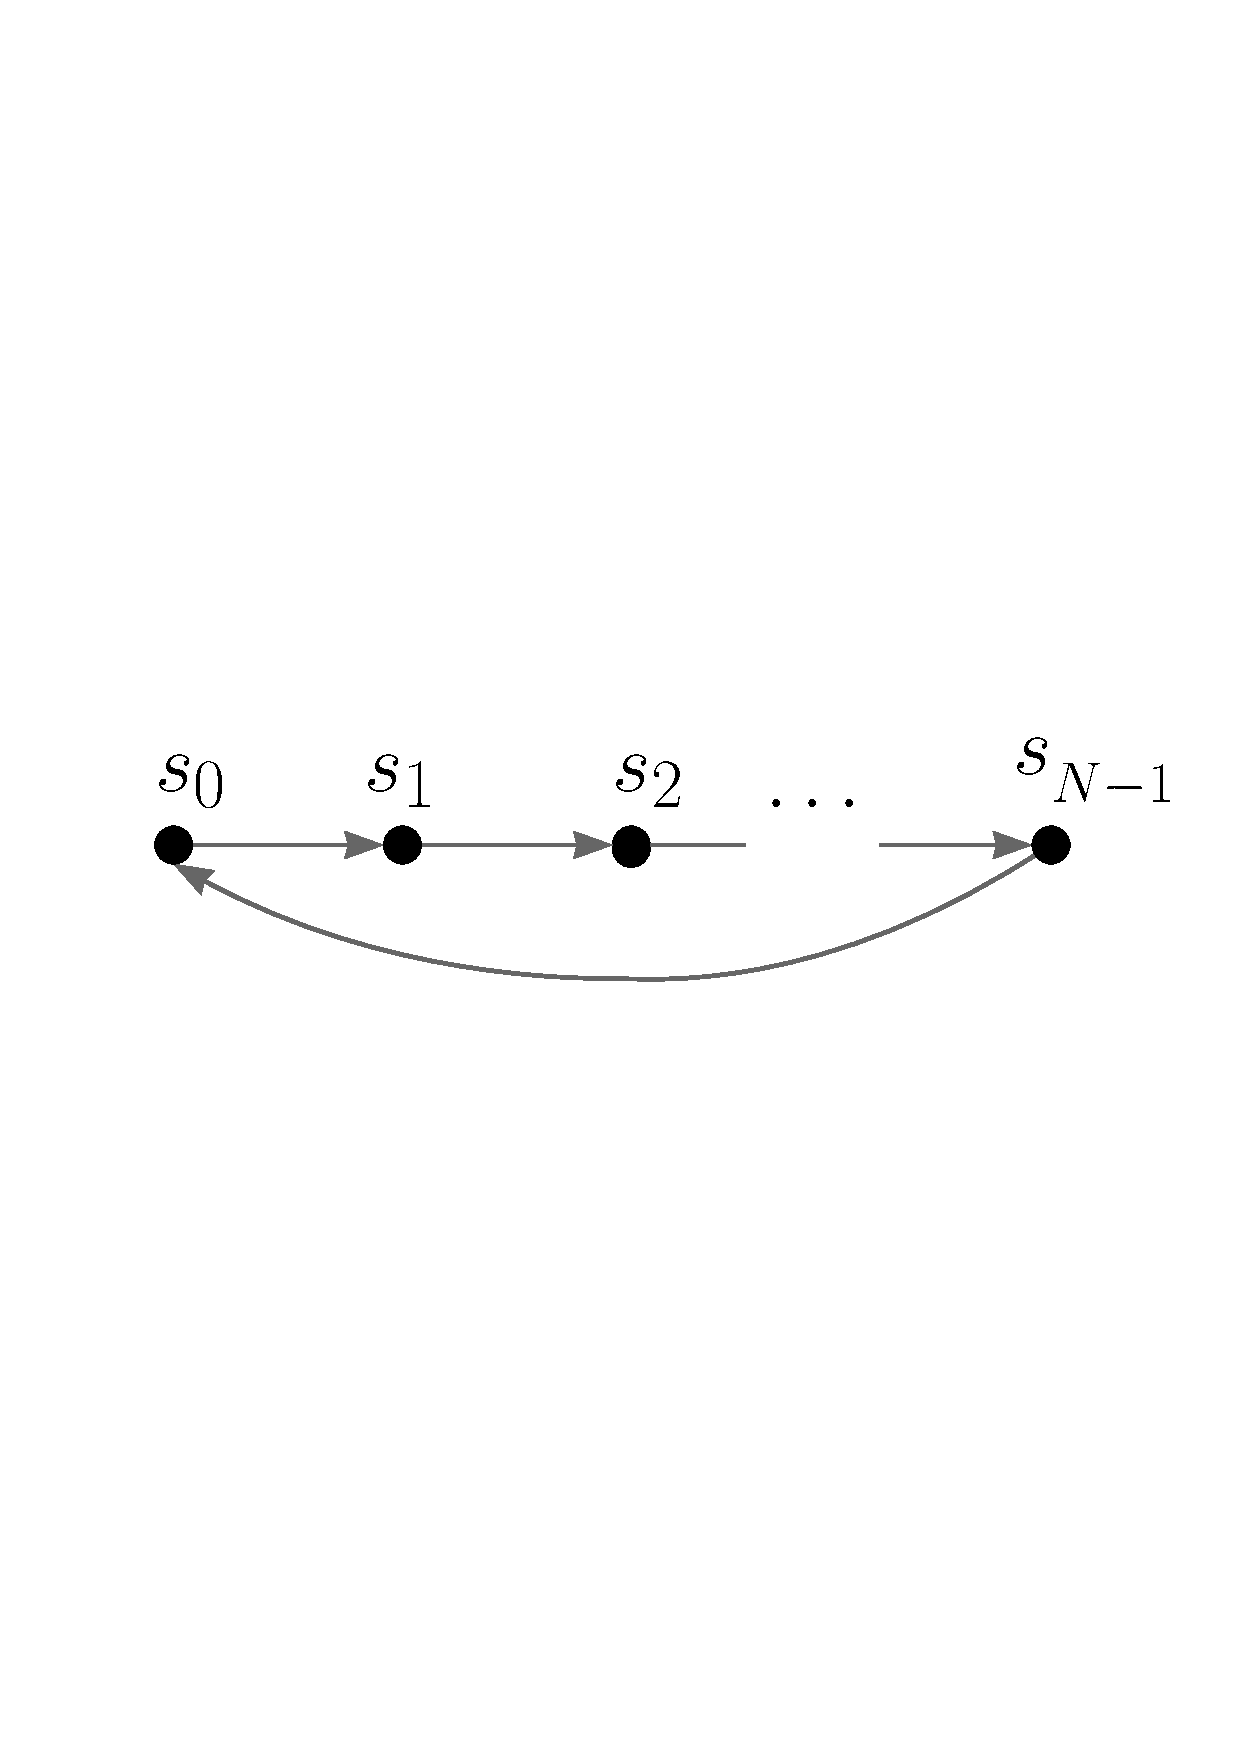
\includegraphics[width=0.45\linewidth]{Figures/signal_ring_graph_white_border.pdf} }}\hspace{0.2cm}%
%	\qquad
%	\subfloat[t][\label{figb_graphs}]{{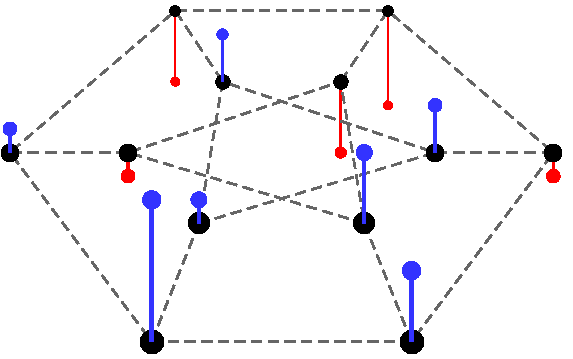
\includegraphics[width=0.4\linewidth]{Figures/signal_duher_graph.pdf} }}\\
%	\subfloat[\label{figc_graphs}]{{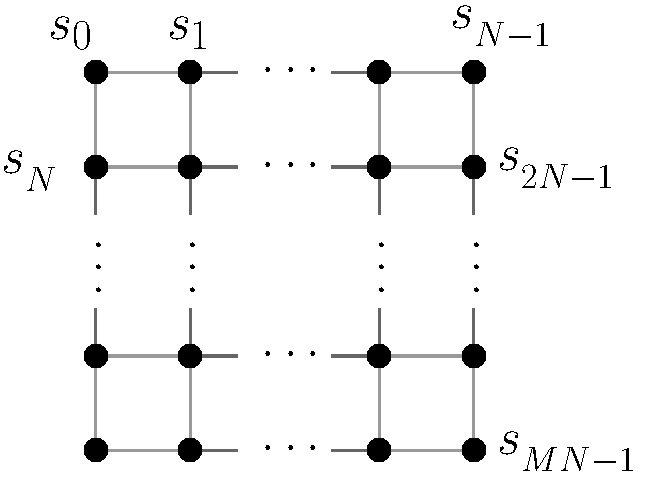
\includegraphics[width=0.45\linewidth]{Figures/image_graph.pdf} }}%
%	\subfloat[\label{figd_graphs}]{{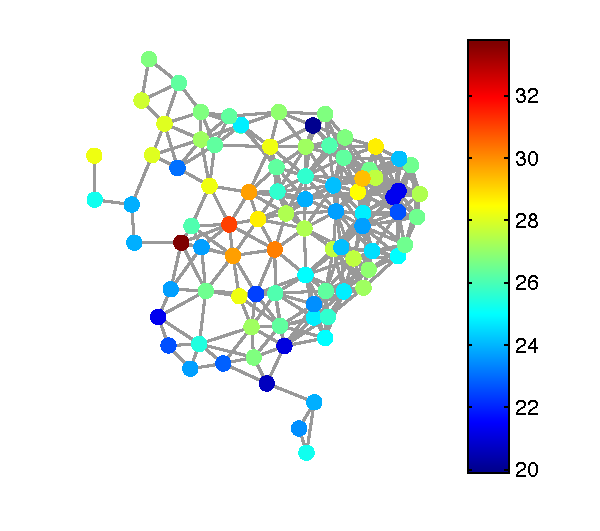
\includegraphics[width=0.4\linewidth]{Figures/graph_temp_bulbo_seco_NE_00h_01Fev2012_cropped.pdf} }}%
%	\caption{Exemplos de representa\c{c}\~oes de sinais sobre (a) um grafo em anel direcionado, (b) um grafo de D\"{u}her n\~ao-direcionado, (c) um grafo n\~ao-direcionado em forma de rede retangular uniforme  e (d) um grafo formado por cidades do Nordeste brasileiro.}%
%	\label{fig:graphs}%
%	\vspace{-0.2cm}
%\end{figure}
\begin{equation}\label{eq:C}
\mathbf{C} =
\begin{bmatrix}
&  &  &   1\\ 
1 &  &   & \\ 
&   \ddots &  & \\ 
&  &   1 & 
\end{bmatrix},
\end{equation}
\noindent and plays an essential role in GSP: if a signal $ \mathbf{x} = (x_0 \ x_1 \ \dots \ x_{N-1})^T $ defined on a ring graph is left multiplied by the adjacency matix, one has $ \widetilde{\mathbf{x}} = (s_{N-1} \ x_0 \ \dots \ s_{N-2})^T $; that is,
\begin{equation}\label{eq:graph_shift_C}
\widetilde{\mathbf{x}} = \mathbf{C} \mathbf{x}
\end{equation}
\noindent is the result of circularly shifting $ \mathbf{x} $ to the right. This property suggests to generalize the unit shift of a signal on an arbitrary graph as being the left product by the corresponding adjacency matrix,
\begin{equation}\label{eq:graph_shift_A}
\widetilde{\mathbf{x}} = \mathbf{A} \mathbf{x},
\end{equation}
\noindent so that $ \mathbf{A} $ can be interpreted as the graph shift operator. In fact, this operator is a delay \emph{filter} for graph signals.

A filter for signals on a graph with $ |\mathcal{V}| = N $ vertices can be defined as being any matrix $ \mathbf{H} \in \mathbb{C}^{N \times N} $ \cite{sandryhaila2013discrete}. Therefore, every graph filter is linear. On the other hand,
\begin{equation}\label{eq:shift_invariance}
\mathbf{HA}\mathbf{x} = \mathbf{AH}\mathbf{x},\:\:\forall \mathbf{x} \in \mathcal{S} \:\:\Leftrightarrow\:\:\mathbf{HA} = \mathbf{AH},
\end{equation}
\noindent that is, $ \mathbf{H} $ is a linear and shift-invariant (LSI) filter if and only if it commutes with the adjacency matrix $ \mathbf{A} $. The following theorem establishes an important property satisfied by every LSI filter~\cite{sandryhaila2013discrete} .
\vspace{0.2cm}
\begin{theorem}
	\label{theo:01}
	Let $ \mathbf{A} $ be the adjacency matrix of a graph. Let us assume that the characteristic polynomial $char_{\mathbf{A}}(x)$ of $\mathbf{A}$ coincides with the respective minimal polynomial $m_{\mathbf{A}}(x) $. Therefore, $ \mathbf{H} $ is a LSI filter if and only if $ \mathbf{H} $ is a polynomial in $ \mathbf{A} $, i.~e.
	\begin{equation}\label{eq:filtro}
	\mathbf{H} = h(\mathbf{A}) = \sum_{\ell=0}^{L} h_\ell \mathbf{A}^\ell,
	\end{equation}
where $ \mathbf{A}^0 $ is the identity matrix and $ L < \deg(m_{\mathbf{A}}) $.
\end{theorem}

The assumption on $char_{\mathbf{A}}(x)$ and $m_{\mathbf{A}}(x)$ in Theorem~\ref{theo:01} does not hold for all adjacency matrices $\mathbf{A}$. Nevertheless, the result in the referred theorem can be extended to all matrices using the concept of \emph{equivalent graph filters}, as clearly explained in~\cite{sandryhaila2013filters}. In short, for any graph $\mathcal{G} = \{\mathbf{A}, \mathcal{V}\}$, every LSI filter has polynomial representation in $\mathbf{A}$. In this sense, Theorem~\ref{theo:01} suggests a convenient analogy with the classical DSP, since every filter for discrete-time signals can be represented as polynomials evaluated in $ z^{-1} $, the unit delay, via the $z$-transform of its impulse response.

\begin{figure}[t!]
	\centering
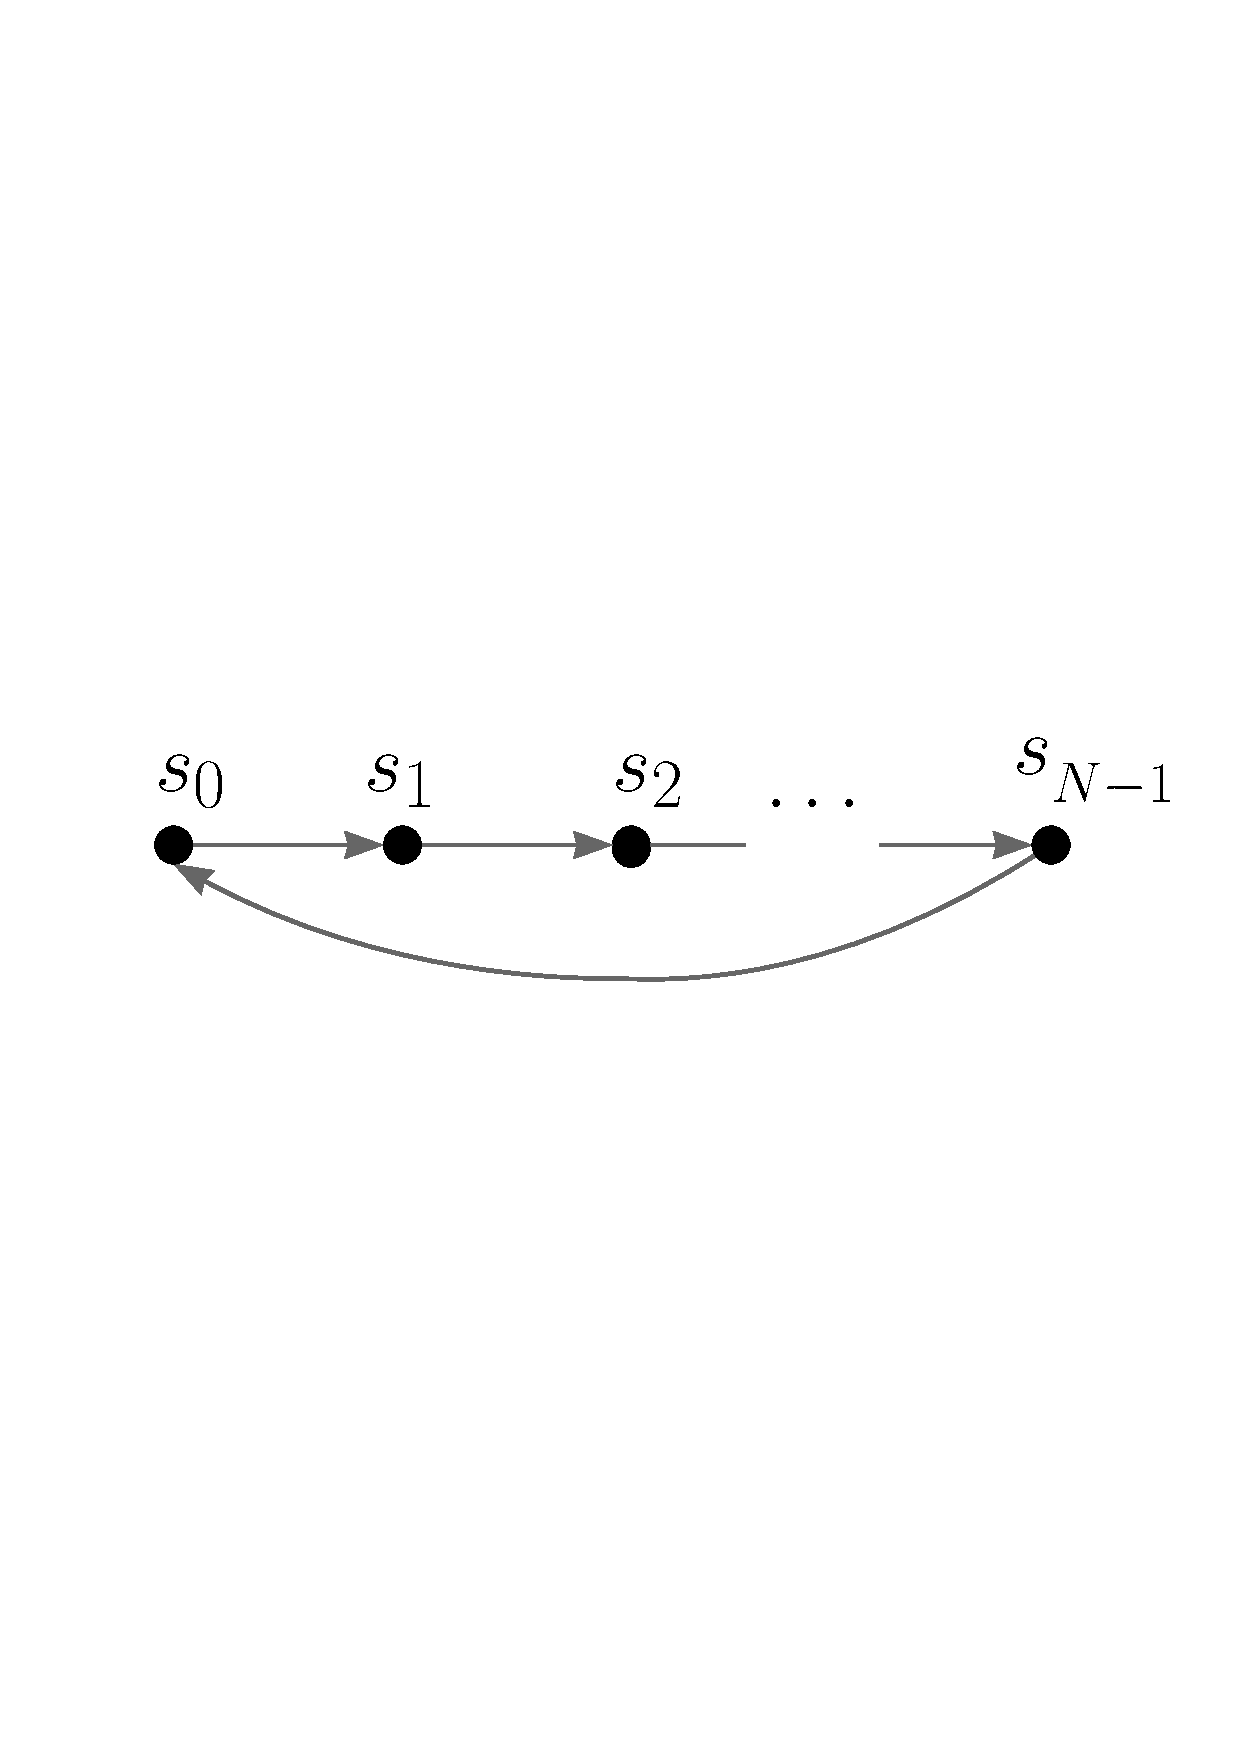
\includegraphics[width=0.6\linewidth]{Figures/signal_ring_graph_white_border.pdf}
	\caption{A directed ring graph.}%
	\label{fig:graphs}%
	\vspace{-0.5cm}
\end{figure}
\subsection{Graph Fourier Transform}

The graph Fourier transform of a signal is its projection on a basis formed by functions invariant to linear and time-invariant (LTI) filtering~\cite{oppenheim1997signals}. Analogously, the graph Fourier transform (GFT) can be defined as the decomposition of a signal on a basis formed by eigenvectors of LSI filtering. Since LSI filters are polynomials in $ \mathbf{A} $ (Theorem \ref{theo:01}), and considering that a matrix and its integer powers share the same eigenvectors, the referred basis coincides with that obtained from the decomposition of $\mathbf{A}$~\cite{sandryhaila2013gft}. In this context, if the corresponding graph has $ N $ vertices, $\mathbf{A} $ admits the Jordan decomposition
\begin{equation}\label{eq:gft_01}
\mathbf{A} = \mathbf{V} \mathbf{J} \mathbf{V}^{-1},
\end{equation}
in which $ \mathbf{V} $ contains the $ N $ Jordan (generalized) eigenvectors of $ \mathbf{A} $ in its columns,
\begin{equation}\label{eq:gft_02}
\mathbf{V} = \left(\mathbf{v}_0 \ \mathbf{v}_1 \ \dots\ \mathbf{v}_{N-1}\right),
\end{equation}
and $\mathbf{J}$ is a block diagonal matrix formed of the so-called Jordan blocks. In particular, if $\mathbf{A}$ is diagonalizable, (\ref{eq:gft_01}) coincides with its eigendecomposition, so that $\mathbf{J}$ reduces to a diagonal matrix whose entries are the eigenvalues of $\mathbf{A}$.

%Additionally, the subspaces generated by the eigenvectors of a given eigenvalue of $ \mathbf{A} $ are irreducible, have null intersection and have the sum of their dimensions totaling $ N $ \cite{sandryhaila2013gft}. Therefore, $ \mathbf{V} $ provides a basis invariant to LSI filtering for the signal space$ \mathcal{S} $ on the graph having $ \mathbf{A} $ as its adjacency matrix.

In this manner, a signal $ \mathbf{x} \in \mathcal{S} $ can be decomposed into its components on the basis $ \mathbf{V} $ as
\begin{align}\label{eq:GFT_inv}
\mathbf{x} &= \widehat{x}_0 \mathbf{v}_0 + \dots + \widehat{x}_{N-1} \mathbf{v}_{N-1} \notag \\
&= \mathbf{V} (\widehat{x}_0 \ \widehat{x}_1 \ \dots \ \widehat{x}_{N-1})^T \notag \\
&= \mathbf{V} \widehat{\mathbf{x}}.
\end{align}
The last expression is then defined as being the synthesis equation of the graph Fourier transform. Consequently, the GFT analysis equation is
\begin{equation}\label{eq:GFT_fwd}
\widehat{\mathbf{x}} = \mathbf{V}^{-1} \mathbf{x}.
\end{equation}

For discrete-time signals, it has been remarked that the corresponding domain can be modeled as a directed ring graph with edges having unitary weights and, therefore, with adjacency matrix $ \mathbf{C} $ given in~(\ref{eq:C}). Since $ \mathbf{C} $ is circulant, it is diagonalized by the discrete Fourier transform (DFT) matrix $ \mathbf{F} $. Thus, one has
\begin{equation}\label{eq:diag_C}
\mathbf{C} = \mathbf{F}^{-1} \mathbf{\Lambda}_{\mathbf{C}} \mathbf{F},
\end{equation}
where $$ \mathbf{\Lambda}_{\mathbf{C}} = \text{diag}\left(
1 \:\
e^{-j \frac{2\pi}{N}} \:\:\
e^{-j \frac{4\pi}{N}}\:\: \
e^{-j \frac{6\pi}{N}} \:\: \cdots \:\:
e^{-j \frac{2\pi (N-1)}{N}}
\right).$$In this case, the GFT matrix becomes $ \mathbf{V}^{-1} = \mathbf{F} $, evidencing the desirable property that the GFT of discrete-time signals coincides with the DFT.

\vspace{0.25cm}
\noindent\textbf{Frequency response of graph filters.} In order to understand how a graph filter acts on the GFT domain, identified as frequency domain,~(\ref{eq:gft_01}) and Theorem \ref{theo:01} are used. The response of the filter $ \mathbf{H} =\sum_{\ell=0}^{L} h_\ell \mathbf{A}^\ell $ to the signal $ \mathbf{x} $ is given by
\begin{align}\label{eq:resposta_freq_01}
\mathbf{H} \mathbf{x} &= \sum_{\ell=0}^{L} h_\ell \mathbf{A}^\ell \mathbf{x} =
\sum_{\ell=0}^{L} h_\ell \left(\mathbf{V} \mathbf{J} \mathbf{V}^{-1}\right)^\ell \mathbf{x} \notag \\[0.5em]
&= \mathbf{V} \left(\sum_{\ell=0}^{L} h_\ell \mathbf{J}^\ell \right) \mathbf{V}^{-1} \mathbf{x}.
\end{align}
Taking the GFT of both sides of the last equation, one has
\begin{equation}\label{eq:resposta_freq_02}
\mathbf{V}^{-1} \mathbf{H} \mathbf{x} =
h(\mathbf{J}) \widehat{\mathbf{x}},
\end{equation}
so that the frequency domain equation corresponding to filtering using $ \mathbf{H} $ is the multiplication by the matrix $ h(\mathbf{J}) $, which represents the frequency response of the filter $ \mathbf{H} $.

\section{Fractional Shift on Graphs}\label{sec:fracshift}
Since the unit shift of a graph signal can be defined as the product by the adjacency matrix of the graph on which it lies, in this work, we propose to define a fractional shift as the product by a non-integer power of $ \mathbf{A} $. Precisely, the signal $\mathbf{x}$ over the graph $\mathcal{G} = \{ \mathbf{A}, {\mathcal{V}} \}$, after being shifted by $a\in[0,1]$, is given by
\begin{equation}
\label{eq:def_frac_delay}
\widetilde{\mathbf{x}}_a = \mathbf{A}^a \mathbf{x}.
\end{equation}
In what follows, we discuss aspects related to the computation of $\mathbf{A}^a$, the interpretation of its application to a graph signal and the consistency of the proposed operator with the classical DSP approach (ideal fractional delay filter).

\subsection{Computation of $\mathbf{A}^{{a}}$}\label{subsec:comp}
The computation of $\mathbf{A}^a$ can be well established by employing results from the theory of matrix functions~\cite{higham2008functions}. In this context, we are interested in evaluating the originally scalar function $f(t)=t^a$, $a\in\mathbb{R}$, but replacing $t$ with $\mathbf{A}$. The most direct way to formally define a function like this uses the Jordan canonical form. With this purpose,~(\ref{eq:gft_01}) is reconsidered; in this equation, the block diagonal matrix $\mathbf{J}$ can be written as
\begin{equation}\label{eq:jcf}
    \mathbf{J}=\textrm{diag}(\mathbf{J}_1,\mathbf{J}_2,\ldots,\mathbf{J}_p),
\end{equation}
where the $k$-th Jordan block $\mathbf{J}_k$ is
\begin{equation}
    \mathbf{J}_k=\mathbf{J}_k(\lambda_k)=\left[\begin{array}{cccc}
    \lambda_k&1&&\\
    &\lambda_k&\ddots &\\
    &&\ddots & 1\\
    &&&\lambda_k
    \end{array}\right]\in\mathbb{C}^{m_k\times m_k}
\end{equation}
and $m_1+m_2+\ldots +m_p=N$. Denote by $\lambda_1,\ldots,\lambda_s$ the distinct eigenvalues of $\mathbf{A}$ and by $n_i$ the \emph{index} of $\lambda_i$ (the order of the largest Jordan block in which $\lambda_i$ appears). The function $f$ is said to be defined on the spectrum of $\mathbf{A}$ if the values
\begin{equation}\label{eq:defspec}
    f^{(j)}(\lambda_i),\quad j=0,1,\ldots,n_i-1,\quad i=1,2,\ldots,s,
\end{equation}
where $f^{(j)}$ denotes the $j^{\textrm{th}}$ derivative of $f$, exist. This is the case of $f(t)=t^a$. The computation of $f(\mathbf{A})=\mathbf{A}^a$ can then be carried out as follows.
\vspace{0.2cm}
\begin{definition}\label{def:jc01}
Let $f$ be defined on the spectrum of $\mathbf{A}\in\mathbb{C}^{N\times N}$ and let $\mathbf{A}$ have the Jordan decomposition~(\ref{eq:gft_01}). Then
\begin{equation}\label{eq:jcf01}
    f(\mathbf{A}):=\mathbf{V}f(\mathbf{J})\mathbf{V}^{-1}=\mathbf{V}\textrm{diag}(f(\mathbf{J}_k))\mathbf{V}^{-1},
\end{equation}
where
\begin{equation}\label{eq:jcf02}
    f(\mathbf{J}_k):=\left[\begin{array}{cccc}
    f(\lambda_k)&f'(\lambda_k)&\cdots &\frac{f^{(m_k-1)}(\lambda_k)}{(m_k-1)!}\\
    &f(\lambda_k)&\ddots &\vdots\\
    &&\ddots & f'(\lambda_k)\\
    &&&f(\lambda_k)\end{array}\right].
\end{equation}
\end{definition}
In the present context, the last definition constitutes a practical way to calculate $\mathbf{A}^a$, because the Jordan form of the adjacency matrix, being necessary for the definition of the corresponding GFT, may already have been computed and thus be available to be used in~(\ref{eq:jcf01}) and~(\ref{eq:jcf02}).


\subsection{Interpreting the graph fractional shift}\label{subsec:interpret}
In order to perform a meaningful interpretation of the graph fractional shift, we consider~(\ref{eq:def_frac_delay}) and the case in which $\mathbf{A}$ is diagonalizable. Using the Jordan decomposition~(\ref{eq:gft_01}), the GFT analysis equation~(\ref{eq:GFT_fwd}) and the computation strategy described in the last subection, we can write
\begin{align}\label{eq:frac_delay_01}
\mathbf{A}^a \mathbf{x} &= \mathbf{V} \mathbf{\Lambda}^a \mathbf{V}^{-1} \mathbf{x} = \mathbf{V}
\begin{bmatrix}
\lambda_1^a &  & \\ 
& \ddots & \\ 
&  & \lambda_N^a
\end{bmatrix}
\widehat{\mathbf{x}} \notag \\[0.5em]
&= \mathbf{V} (\widehat{\mathbf{h}}_a \odot \widehat{\mathbf{x}}) = \text{GFT}^{-1} \{\widehat{\mathbf{h}}_a \odot \widehat{\mathbf{x}}\},
\end{align}
where $\widehat{\mathbf{h}}_a := (\lambda_1^a \ldots \lambda_N^a)$ and $\odot$ represents the point-wise vector product.

Equation~(\ref{eq:frac_delay_01}) shows that $ \mathbf{A}^a $ is a graph filter with frequency response $ \text{diag}(\widehat{\mathbf{h}}_a) $; moreover, if $ \mathbf{x} $ is an $N$-point discrete-time signal (case in which the GFT coincides with the DFT), one observes that the filter in the DFT domain is the vector $ \widehat{\mathbf{h}}_a $ itself. In this case, it has been discussed that the adjacency matrix of the respective graph is diagonalized according with~(\ref{eq:diag_C}), where $ \mathbf{\Lambda}_{\mathbf{C}} $ has as entries the $ N $ roots of unity. The fact that the matrix of eigenvectors of $ \mathbf{C} $ is the Fourier matrix imposes a specific order of the eigenvalues in $ \mathbf{\Lambda}_{\mathbf{C}} $, so that the vector $ \widehat{\mathbf{h}}_a$ is
\begin{align*}
\widehat{\mathbf{h}}_a &= (1 \,\, W_N^a \,\,W_N^{2a}\ldots W_N^{aR} \,\,W_N^{-aR'} \,\,W_N^{a(-R' + 1)}\ldots W_N^{-a}),
\end{align*}
where $ W_N = e^{-j \frac{2\pi}{N}} $ and
\begin{equation}
\begin{cases}
R = \frac{N-1}{2} \text{ and } R' = R, & \text{ if } N \text{ is odd},\vspace{0.2cm} \\
R = \frac{N}{2} - 1 \text{ and } R' = R+1, & \text{ if } N \text{ is even},
\end{cases}
\end{equation}
$n=0,1,\ldots,N-1$. It can be shown that the inverse DFT of $ \widehat{\mathbf{h}}_a $ has components given by~(\ref{eq:DFT_inversa_autovalores}).

\begin{figure}[b]
	\centering
	\subfloat[\label{figa_frac_delay_directed}]{{
			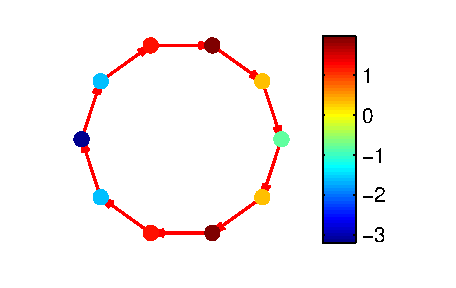
\includegraphics[width=0.40\linewidth]{Figures/d170309_frac_delay_ring_visualization_V5_a.eps}
			}}
	%	\vspace{-0.2cm}
	\subfloat[\label{figb_frac_delay_directed}]{{
			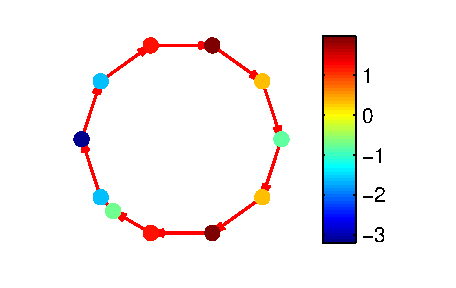
\includegraphics[width=0.40\linewidth]{Figures/d170309_frac_delay_ring_visualization_V5_b.eps}
			}}\\
	\subfloat[\label{figc_frac_delay_directed}]{{
			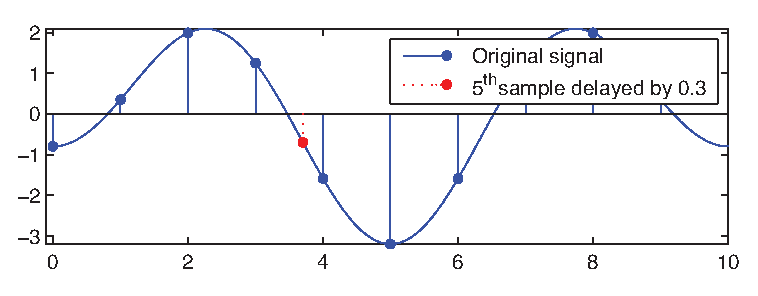
\includegraphics[width=0.85\linewidth]{Figures/d170309_frac_delay_ring_visualization_V5_c1.eps}
			}}% 
	\caption{Fractional shift by $a=0{.}3 $ of a sample of a signal on a directed ring graph with unit weights. (a) Original signal on a directed ring graph. (b) Graph in which the 5$\textsuperscript{th}$ sample delayed by $a=0{.}3 $ appears as an interpolated sample between the 4$\textsuperscript{th}$ and the 5$\textsuperscript{th}$ samples of the original signal. (c) Original discrete signal and the delayed sample.}
	\label{fig:frac_delay_directed}
	%\vspace{-0.3cm}
\end{figure}

\begin{figure*}[h!]
\begin{equation}\label{eq:DFT_inversa_autovalores}
h_a[n]\hspace{-0.03cm}=\hspace{-0.03cm}
\left\{\begin{array}{ll}
%\displaystyle
{\dfrac{1}{N}} \dfrac{\sin (\pi (n-a))}{\sin \left(\frac{\pi}{N} (n-a)\right)}, &\text{ if $N$ is odd},\vspace{0.25cm}\\
%\displaystyle
{\dfrac{1}{N} \cot \left(\dfrac{\pi}{N} (n-a)\right) \sin (\pi (n-a))}{+ \dfrac{j}{N} (-1)^n \sin (\pi a)}, &\text{ if } N \text{ is even}.
\end{array}\right.
\end{equation}
\hrule
\end{figure*}

The product by a fractional power of the adjacency matrix produces the effect illustrated in Fig. \ref{fig:frac_delay_directed}, for a directed ring graph; it can be seen, for example, how the 5\textsuperscript{th} sample of the signal shifted by $a=0{.}3 $ coincides with the value of the continuous-time signal at the same position. On the other hand, the analysis we can perform by observing the \textit{irregular} graph in Fig.~\ref{fig:sinal_Pernambuco} is mostly visual; as we vary the fractional parameter from $0$ (original signal) to $1$, we see in the intermediate snapshots how the signal gradually spreads out from the vertices where, originally, there were already non-zero samples. In this scope, although we employ terms such as delay and shift, which are inherited from classical signal processing, the process observed in the figure looks more like a kind of (fractional) diffusion. In fact, diffusion on graphs have been widely studied~\cite{zhang2008,thanou2017, benzi2021}; it is usually described in terms of a system of ordinary differential equations in time, with the Laplacian matrix of the graph as the coefficient matrix. Fractional diffusion has been used to model certain phenomena that allow long-range interactions and are non-local in nature~\cite{ilic2005,riascos2014,estrada2021,antil2021}. In future works, we intend to investigate the possible relationships between the operator proposed in this paper and the mathematical tools for fractional diffusion in networks. 

Finally, we draw attention to the fact that the signal to be shifted has to be band-limited (see Fig.~\ref{figa_gibbs}). If the signal has abrupt changes in its sample values, this can be viewed as a kind of descontinuity and represents high frequency components, when compared to the predominantly smooth behavior of the signal (see Fig.~\ref{figb_gibbs}). As a consequence, we can observe considerable fluctuations around the disparate samples when the signal is fractionally delayed, an effect similar to the Gibbs phenomenon.

\begin{figure}[t!]
	\centering
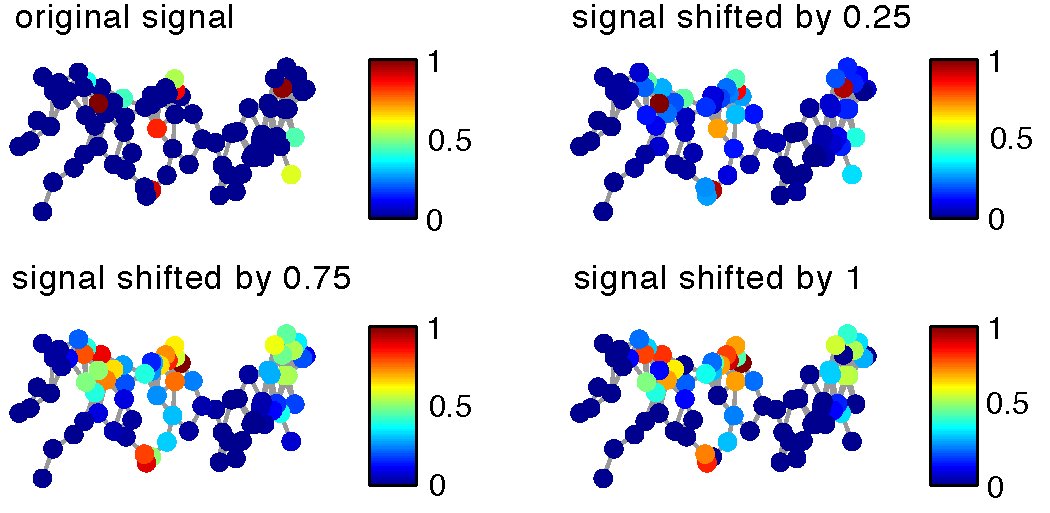
\includegraphics[width=0.95\linewidth]{Figures/signal_PE_V2_PT.pdf}
	\caption{Fractional shift of a signal, (originally) with $10$ non-zero samples, defined on a graph formed by $80$ cities of Pernambuco state, Brazil. Note that the shifted signal is similar to the original signal, if $ a $ is close to $0$, and similar to the unit-shifted signal, if $ a $ is close to $1$.}%
	\label{fig:sinal_Pernambuco}%
	\vspace{-0.2cm}
\end{figure}

\begin{figure}[t!]
	\centering
	\subfloat[\label{figa_gibbs}]{{
			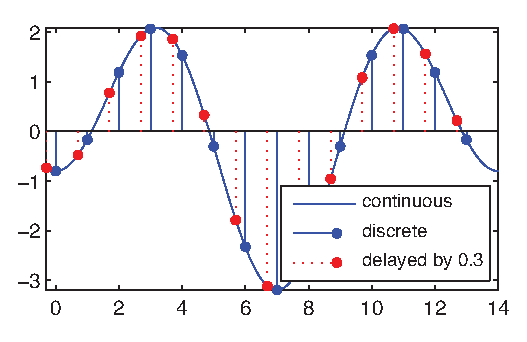
\includegraphics[width=0.8\linewidth]{Figures/d170309_frac_delay_ring_visualization_V2_no_gibbs.eps}
			}}\\
	%	\vspace{-0.2cm}
	\subfloat[\label{figb_gibbs}]{{
			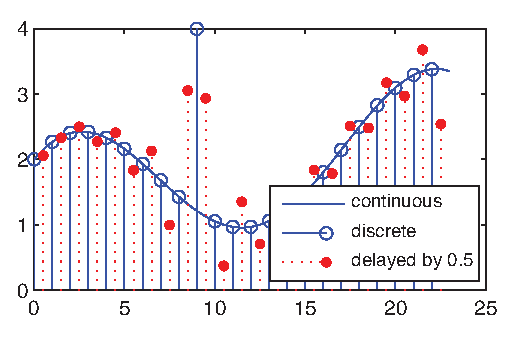
\includegraphics[width=0.78\linewidth]{Figures/frac_delay_ring_TESTS_gibbs_effect.eps}
			}}%
	\caption{Fractional shift for a signal (a) without and (b) with abrupt variations (descontinuities).}%
	\label{fig:frac_delay_gibbs}%
	\vspace{-0.2cm}
\end{figure}

\subsection{Consistency with classical approach: the ideal fractional delay filter}\label{subsec:consist}
In the classical approach to the problem of fractionally shifting a discrete-time signal, the continuous-time version of the signal can be reconstructed by shifting and then resampling with the same sample period~\cite{alan1989discrete,valimaki1995discrete}. Due to the Nyquist-Shannon Theorem, this procedure requires that the signal is band-limited. In this context, it can be shown that, if a discrete-time signal $ \mathbf{x} $ is band-limited, its version shifted by $ a \in [0,1] $ is
$$
x[n-a] = \sum_k x[k] \mathrm{sinc} (n - k - a),
$$
so that the (ideal low-pass) filter used to perform the referred shift has components
\begin{equation}
h_{_{LPF}}[n] = \mathrm{sinc} (n-a).
\end{equation}

The filter $ \mathbf{h}_{_{LPF}} $ is non-causal and unstable (it is not BIBO -- \emph{bounded input, bounded output}, because its impulse response has infinite energy) and, therefore, it is not physically realizable. In this way, fractional delay filter implementations should just \emph{approximate} $ \mathbf{h}_{_{LPF}} $ as much as possible.

In order to evaluate how close to $ h_{_{LPF}}[n] = \mathrm{sinc} (n-a) $, $ 0\leq a \leq 1 $, is $h_a[n]$, for odd $N$ (see the first row of~(\ref{eq:DFT_inversa_autovalores})), the point-wise difference between these signals has been computed for different values of $ N \in [10^1, 10^6]$. In Fig. \ref{fig:convergence}, we show the relative error  (ratio between the energy of the error $(\mathbf{h}_a - \mathbf{h}_{_{LPF}})$ and that of $ \mathbf{h}_{_{LPF}} $), in terms of $ N $ and $a $.

The result suggests that, in fact, $ \mathbf{h}_a $ converges in the mean in $ \ell^2 $ to $ \mathbf{h}_{_{LPF}}$ as $ N $ grows, with relative error less than $ 5\% $ for $ N \approx 30 $. Moreover, the error is greater when $ a $ is close to $ 0{.}5 $, being negligible or null when $ a $ is an integer. In fact, the error is exactly zero for $ a=0$ (or $a=1$) and $ n = a $, since
\begin{equation}\label{eq:lim_h_impar}
\lim_{n \rightarrow a} h_{a}[n] = 1
\Rightarrow
\lim_{n \rightarrow a} \big(h_{a}[n] - \mathrm{sinc}(n-a)\big) = 0.
\end{equation}

The same result is obtained for even $N$, starting from the second row of~(\ref{eq:DFT_inversa_autovalores}). When $a$ is non-integer, $h_a[n] $ is complex, with imaginary part of constant modulus for a fixed $a$. Considering the corresponding real part only, the error was smaller than that taking into account also the contribution of the imaginary part. Fig. \ref{fig:convergence_even_N_real_part} and Fig. \ref{fig:convergence_even_N_abs} show that the errors with and without the imaginary part equally decay as  $ N $ grows, but, using the real part only, the results are significantly better.

\begin{figure}[ht!]
	\centering
	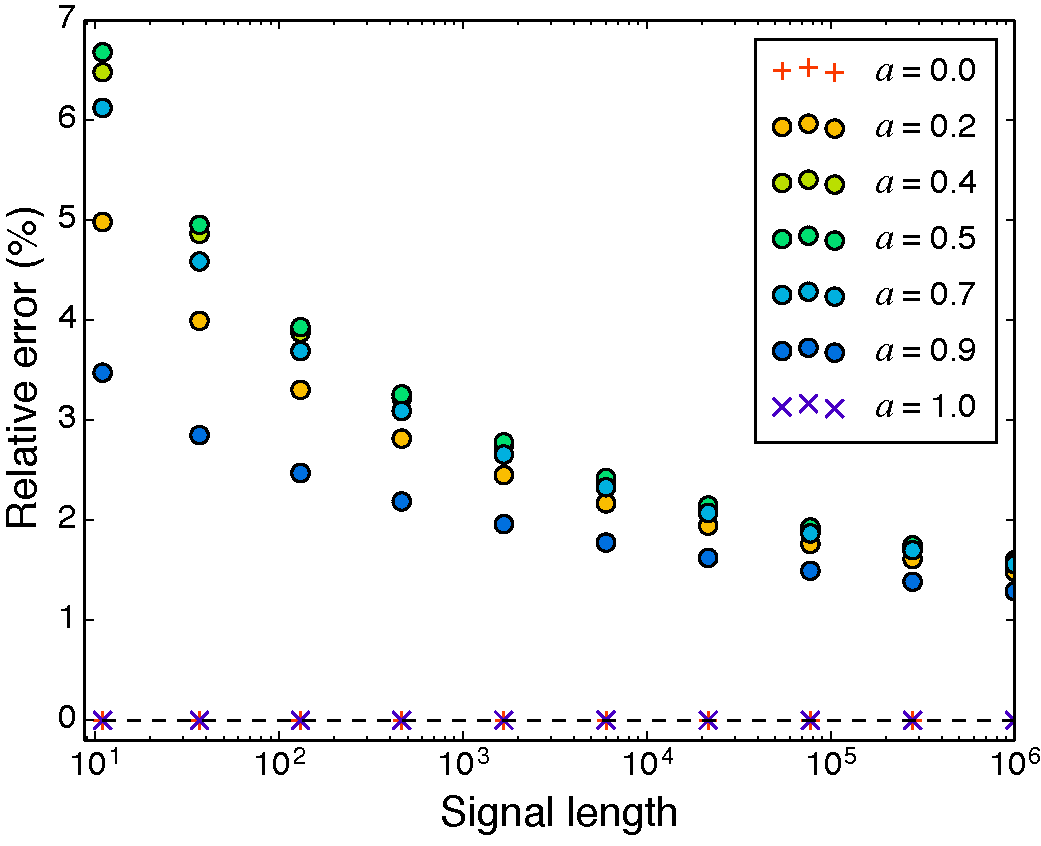
\includegraphics[width=0.81\linewidth]{Figures/convergence_odd_N_V4.pdf}
	\caption{Percent error (normalized by the energy of $ \mathbf{h}_{_{LPF}} $) of $ \mathbf{h}_a $ related to $ \mathbf{h}_{_{LPF}} $, for different (odd) values of $ N $ and the fractional shift parameter $ a $.}
	\label{fig:convergence}
\end{figure}

\begin{figure}[ht!]
	\centering
	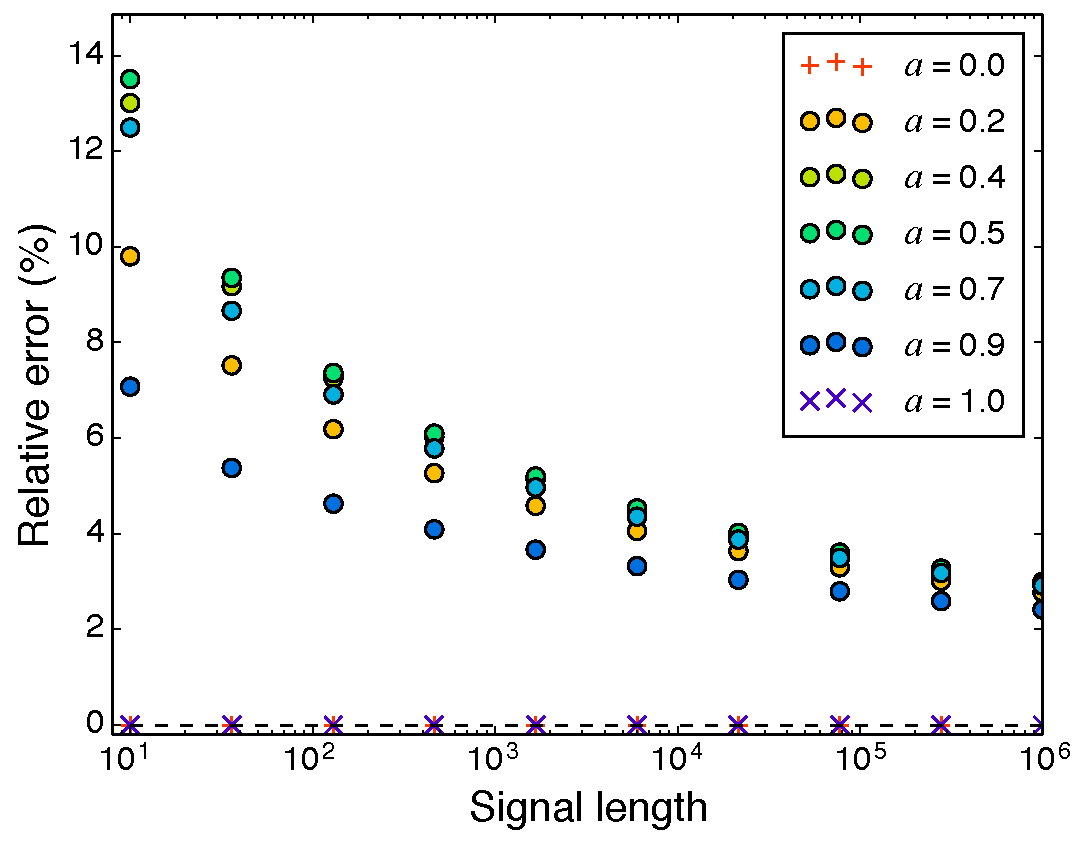
\includegraphics[width=0.81\linewidth]{Figures/convergence_even_N_real_part.pdf}
	\caption{Relative mean error between $ \mathcal{R}e\{\mathbf{h}_a\} $ and $ \mathbf{h}_{_{LPF}} $ for $ N $ even, in terms of the fractional shift parameter $a$.}
	\label{fig:convergence_even_N_real_part}
\end{figure}

\begin{figure}[ht!]
	\centering
	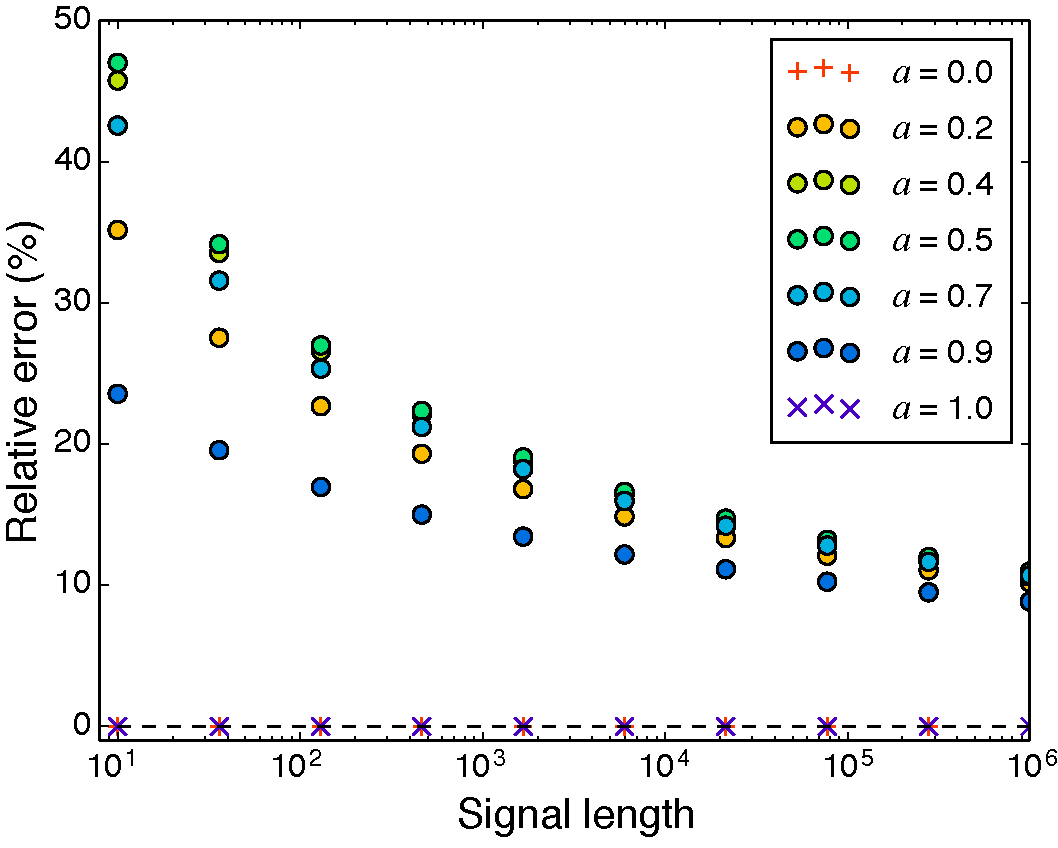
\includegraphics[width=0.81\linewidth]{Figures/convergence_even_N_abs_V2.pdf}
	\caption{Modulus of the relative mean error between $ \mathbf{h}_a $ and $ \mathbf{h}_{_{LPF}} $ for $ N $ even, in terms of the fractional shift parameter $a$.}
	\label{fig:convergence_even_N_abs}
	\vspace{-0.3cm}
\end{figure}

\subsection{Polynomial representation}\label{subsec:poly}
The fractional shift matrix $ \mathbf{A}^a$ necessarily commutes with $ \mathbf{A} $, because $ \mathbf{A}^a\mathbf{A} = \mathbf{A}^{1 + a} = \mathbf{A}\mathbf{A}^a  $, so that $ \mathbf{A}^a $ is an LSI filter for signals on graphs having  $ \mathbf{A} $ as adjacency matrix (see~(\ref{eq:shift_invariance})). Therefore, according to Theorem~\ref{theo:01}, $\mathbf{A}^a$ admits a polynomial representation like the one given in~(\ref{eq:filtro}). In what follows, we evaluate such a possibility for directed ring graphs and for arbitrary graphs.

\vspace{0.25cm}
\noindent\textbf{Directed ring graphs.} The adjacency matrix $ \mathbf{C} $ in~(\ref{eq:C}) of the directed ring graph with unitary weights satisfies $ char_\mathbf{C} = m_\mathbf{C} $ (due to the fact that the eigenvalues of  $\mathbf{C}$ are distinct). Therefore $ \mathbf{H} = \mathbf{C}^a $ can be directly expressed as a polynomial of degree up to  $(N-1)$ in $ \mathbf{C} $. In order to do this, we consider ~(\ref{eq:diag_C}) and the fact that $ \mathbf{F}^{-1} = \mathbf{F}^H $, with $ H $ indicating the conjugate transpose. This allows to show that  $ \mathbf{C}^a = \mathbf{F}^{H} \mathbf{\Lambda}^a_{\mathbf{C}} \mathbf{F}$ is a circulant matrix with the first column given by $ \mathbf{h}_a $ in (\ref{eq:DFT_inversa_autovalores}). Moreover, since the left product of a matrix by $\mathbf{C}$ produces a circular down-shift in each column of the matrix, the $ N $ powers of $\mathbf{C}$ form a basis for the space of $N\times N $ circulant matrices (note that $\mathbf{C}^N =  \mathbf{C}^0$ is the identity matrix). From the above, we conclude that the coefficients of the polynomial representation of $ \mathbf{C}^a $ are the entries of $ \mathbf{h}_a $, i.~e.
\begin{equation}\label{eq:poly_C}
\mathbf{H} = \mathbf{C}^a = \sum_{\ell=0}^{N-1} h_a[\ell] \mathbf{C}^\ell.
\end{equation}

%\subsection{Fun\c{c}\~oes de matrizes}
%
%A teoria de \emph{fun\c{c}\~oes de matrizes} ser\'a aqui utilizada no sentido de mapeamentos $ f: \mathbb{C}^{n \times n}  \rightarrow \mathbb{C}^{n \times n}$ que generalizam, de certa forma, as respectivas fun\c{c}\~oes $ f $ de argumento escalar \cite{higham2008functions}. Pretende-se mostrar a seguir que, utilizando essa teoria, encontra-se para o filtro de deslocamento fracion\'ario proposto uma express\~ao polinomial na matriz de adjac\^encia, de forma que ele \'e LSI. Formalmente, define-se uma fun\c{c}\~ao de matriz como segue \cite{lima2014fractional}.
%
%\begin{definicao}\label{def:01}
%	Seja $ f $ uma fun\c{c}\~ao definida sobre os autovalores de uma matriz $ \mathbf{A} $, de dimens\~ao $ N \times N $, com polin\^omio m\'inimo $ m_{\mathbf{A}}(x) $. Sejam $ \lambda_1, \lambda_2, \dots, \lambda_v $ os autovalores distintos de $ \mathbf{A} $, e $ n_i $ a dimens\~ao do maior bloco de Jordan no qual $ \lambda_i $ aparece. Ent\~ao a fun\c{c}\~ao $ f $ sobre $ \mathbf{A} $ \'e definida como	
%	\begin{equation}\label{eq:matrix_function_01}
%	f(\mathbf{A}) \coloneqq r(\mathbf{A}),
%	\end{equation}
%em que $ r $ \'e o polin\^omio de grau menor que $ \deg m_A $ que satisfaz a interpola\c{c}\~ao
%	\begin{align}\label{eq:matrix_function_02}
%	r^{(j)}(\lambda_i) = f^{(j)}(\lambda_i), \quad
%	&j = 0, 1, \dots, n_i -1 \notag \\
%	&i = 1, 2, \dots, v.
%	\end{align}
%	
%	Se $ n_i = 1 \ \forall i $, $ r $ \'e o polin\^omio interpolador de Lagrange,	
%	\begin{equation}\label{eq:matrix_function_03}
%	r(x) = \sum_{i = 1}^{v} f(\lambda_i) \ell_i (x), \quad
%	\ell_i(x) = \prod_{\substack{k = 1 \\ k \neq i}}^{v} \frac{x - \lambda_k}{\lambda_i - \lambda_k}.
%	\end{equation}
%\end{definicao}
%
%Pode-se mostrar que, para a matriz de adjac\^encia do grafo direcionado em anel com pesos unit\'arios $ \mathbf{C} $, a fun\c{c}\~ao de matriz que generaliza $ f(x) = x^a $, $ 0 \leq a \leq 1 $, \'e
%
%{\color{red} Falta terminar os c\'alculos!}

\noindent\textbf{Arbitrary graphs.} In order to demonstrate how to obtain the polynomial representation of $\mathbf{H}=\mathbf{A}^a$ for arbitrary graphs, we consider another strategy to compute matrix functions. We first remember that, by definition, the minimal polynomial $m_{\mathbf{A}}(t)$ of $\mathbf{A}$ is the unique monic polynomial of lowest degree such that $m_{\mathbf{A}}(\mathbf{A})=\mathbf{0}$. By considering the Jordan canonical form of $\mathbf{A}$, it can be seen that
\begin{equation}
m_{\mathbf{A}}(t)=\prod_{i=1}^s (t-\lambda_i)^{n_i}.
\end{equation}
It follows immediately that $m_{\mathbf{A}}$ is zero on the spectrum of $\mathbf{A}$, that is, the values computed in~(\ref{eq:defspec}) are all zero for $f(t)=m_{\mathbf{A}}(t)$. Given any polynomial $p$ and any matrix $\mathbf{A}\in\mathbb{C}^{N\times N}$, $p$ is clearly defined on the spectrum of $\mathbf{A}$ and $p(\mathbf{A})$ can be defined by substitution. For polynomials $p$ and $q$, $p(\mathbf{A})=q(\mathbf{A})$ if and only if $p$ and $q$ take the same values on the spectrum. Thus the matrix $p(\mathbf{A})$ is completely determined by the values of $p$ on the spectrum of $\mathbf{A}$. The following definition can then be established.
\vspace{0.2cm}
\begin{definition}\label{def:jc02}
Let $f$ be defined on the spectrum of $\mathbf{A}\in\mathbb{C}^{N\times N}$. Then $f(\mathbf{A}):=p(\mathbf{A})$, where $p$ is the unique polynomial of degree less than $\sum_{i=1}^s n_i$ (which is the degree of the minimal polynomial) that satisfies the interpolation conditions
\begin{equation}
    p^{(j)}(\lambda_i)=f^{(j)}(\lambda_i),\quad j=0:n_i-1,\quad i=1:s.
\end{equation}
\end{definition}

The polynomial $p$ above is known as the Hermite interpolating polynomial. In particular, if $n_i=1$, $i=1,\ldots,s$, $p$ corresponds to the Lagrange interpolating polynomial
\begin{equation}
    p(t)=\sum_{i=1}^s f(\lambda_i)l_i(t),\quad l_i(t)=\prod_{j=1,j\neq i}^s \left(\frac{t-\lambda_j}{\lambda_i-\lambda_j}\right).
\end{equation}
In any case, the results briefly presented above lead us to conclude that $\mathbf{A}^a$ can be expressed as a polynomial in $\mathbf{A}$ and, therefore, according to Theorem~\ref{theo:01}, the fractional shift of a graph signal can be implemented as a LSI graph filter.

\section{Numerical Results}\label{sec:num}
In the last section, we have discussed the effect of applying a fractional shift to a graph signal and demonstrated that $\mathbf{A}^a$ admits a polynomial representation. In the first part of this section, we develop a small numerical example to illustrate how the referred representation can be obtained. Secondly, we consider a possibility that, for practical purposes, seems to allow better exploiting the potential for generalization of the proposed fractional operator: replacing $\mathbf{A}$ with $\mathbf{A}^a$ in~(\ref{eq:filtro}) when designing a graph filter. Naturally, the resulting filter, being a polynomial in $\mathbf{A}^a$, could also be expressed as a polynomial in $\mathbf{A}$ and, therefore, it is a LSI filter.

\subsection{Example: Polynomial Representation of $\mathbf{A}^{a}$}\label{subsec:num1}
The graph considered in this example is shown in Fig.~\ref{fig:polyrepres} and has adjacency matrix
\begin{equation}\label{eq:ex001}
%\setlength{\arraycolsep}{3pt}
\mathbf{A}=\left[\begin{array}{ccccc}
5 & 4 & 2 & 1 \\
0 & 1 & -1 & -1\\
-1 & -1 & 3 & 0\\
1 & 1 & -1 & 2
\end{array}\right].
\end{equation}
The entries of $\mathbf{A}$ in~(\ref{eq:ex001}) were chosen so that the Jordan decomposition of such a matrix had integer entries only. The referred decomposition is written using matrices
\begin{equation}\nonumber
%\setlength{\arraycolsep}{3pt}
\mathbf{V}=\left[\begin{array}{ccccc}
-1 & 1&1&1\\
1&-1&0&0\\
0&9&-1&0\\
0&1&1&0
\end{array}\right],\:\:
%\setlength{\arraycolsep}{3pt}
\mathbf{V}^{-1}=\left[\begin{array}{ccccc}
0&1&1&1\\
0&0&1&1\\
0&0&-1&0\\
1&1&1&0
\end{array}\right]
\end{equation}
and
\begin{equation}
%\setlength{\arraycolsep}{3pt}
\mathbf{J}=\left[\begin{array}{ccccc}
1&0&0&0\\
0&2&0&0\\
0&0&4&1\\
0&0&0&4
\end{array}\right].
\end{equation}
Considering $f(t)=t^{0.3}$ and Definition~\ref{def:jc01}, $f(\mathbf{A})=\mathbf{A}^{0.3}$ can be computed according to
\begin{equation}\nonumber
%\setlength{\arraycolsep}{2.5pt}
\mathbf{A}^{0.3}=\mathbf{V}
\left[\begin{array}{ccccc}
f(1)&0&0&0\\
0&f(2)&0&0\\
0&0&f(4)&f'(4)\\
0&0&0&f(4)
\end{array}\right]\mathbf{V}^{-1},
\end{equation}
which gives
\begin{equation}\nonumber
%\setlength{\arraycolsep}{2.5pt}
\mathbf{A}^{0.3}=
\left[\begin{array}{ccccc}
    1.6294  &  0.6294 &   0.3448 &   0.2311\\
         0  &  1.0000 &  -0.2311 &  -0.2311\\
   -0.1137 &  -0.1137  &  1.4020     &    0\\
    0.1137  &  0.1137  & -0.1709  &  1.2311
\end{array}\right].
\end{equation}
The same result can be achieved by using Definition~\ref{def:jc02}, which gives
\begin{align}
    p(\mathbf{A})&=f(\mathbf{A})=\mathbf{A}^{0.3}\nonumber\\
    &=0.6688\mathbf{I}+0.3915\mathbf{A}-0.0654\mathbf{A}^2+0.0051\mathbf{A}^3,\nonumber
\end{align}
the polynomial representation of $\mathbf{A}^{0.3}$.

\begin{figure}
	\centering
	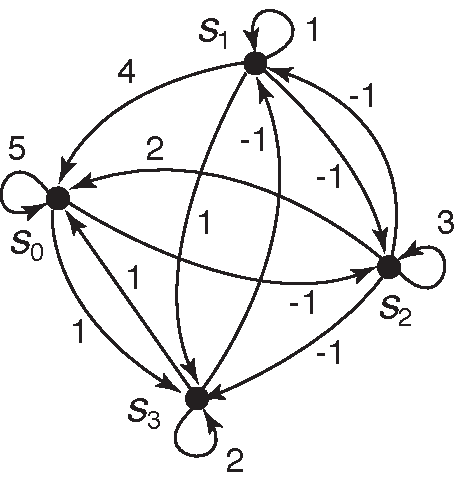
\includegraphics[width=0.55\linewidth]{Figures/graph_jordan.pdf}
	\caption{Directed graph used to illustrate how the corresponding fractional shift operator can be computed and represented in polynomial form.}
	\label{fig:polyrepres}
\end{figure}

\subsection{Least-Square approximation of LSI filters}\label{subsec:lsi}
Before developing a numerical example illustrating the use of $\mathbf{A}^a$ to filter graph signals, we first review a simple design technique that are least-squares approximations of ideal LSI filters~\cite{sandryhaila2014frequency}. Such a method consists of defining the (ideal) filter by specifying the values of $h(\lambda_i)$ (filter response in each eigenvalue of the shift operator), instead of determining the values of $h_{\ell}$ (filter coefficients). Describing the frequency response of the filter for each eigenvalue  $ \lambda_i $, we obtain the linear system of equations
\begin{equation}
\label{eq:siseq}
\begin{aligned}
h(\lambda_0) &= \alpha_0, \\
h(\lambda_1) &= \alpha_1, \\
&\vdots \\
h(\lambda_{N-1}) &= \alpha_{N-1}, \\
\end{aligned}
\end{equation}
or, since $ h(\cdot) $ is a polynomial of degree $ L $,
\begin{equation}\label{eq:syst01}
\begin{aligned}
h_0 + h_1 \lambda_0 + \dots + h_L \lambda^L_0 &= \alpha_0, \\
h_0 + h_1 \lambda_1 + \dots  + h_L \lambda^L_1 &= \alpha_1, \\
&\vdots \\
h_0 + h_1 \lambda_{N-1} + \dots + h_L \lambda^L_{N-1} &= \alpha_{N-1}. \\
\end{aligned}
\end{equation}
Using a Vandermonde matrix constructed from the eigenvalues $\lambda_i$, the system~(\ref{eq:syst01}) can be written in matrix form as
\begin{equation}\label{eq:siseq2}
\setlength{\arraycolsep}{3pt}
\left[\begin{array}{ccccc}
1 & \lambda_0 & \lambda^2_0 & \dots & \lambda^L_0 \\
1 & \lambda_1 & \lambda^2_1 & \dots & \lambda^L_1 \\
& \vdots & & \vdots & \\
1 & \lambda_{N-1} & \lambda^2_{N-1} & \dots & \lambda^L_{N-1} \\
\end{array}\right]
\begin{bmatrix}
h_0 \\
h_1 \\
\vdots \\
h_L
\end{bmatrix} =
\begin{bmatrix}
\alpha_0 \\
\alpha_1 \\
\vdots \\
\alpha_{N-1}
\end{bmatrix}.
\end{equation}
More specifically, if one desires to design a low-pass filter (LPF) whose cutoff frequency is $ \lambda_{i_\text{cut}} $, one could set
\begin{equation}
\label{eq:alfas}
\left\{\begin{array}{ll}
\alpha_i = 1, & \text{for } j = 0,\ldots, i_\text{cut},\\ 
\alpha_i = 0, & \text{for } j = i_\text{cut}+1,\ldots,N-1.
\end{array}\right.
\end{equation}
Since one generally has $ N \geq L+1$, the system of equations~(\ref{eq:siseq2}) is \emph{overdetermined} and does not have an exact solution. A possible strategy is to find coefficients $ h_\ell $, $ \ell=0, \dots, L-1 $, that minimize, in the least-squares sense, the deviation from the ideal filter response. This corresponds to solve the optimization problem
\begin{equation}
\label{eq:opt}
\underset{\{h_\ell\}_{0, \dots, L-1}}{\text{min}} \left( \sum_{n=0}^{N-1} h(\lambda_n) - \alpha_n \right)^2.
\end{equation}

Our proposal is to replace $\mathbf{A}$ with $\mathbf{A}^a$ in~(\ref{eq:filtro}). If this is performed, the only adjustment needed in the technique described above consists of replacing the eigenvalues $\lambda_i$ with their $a^{\text{th}}$ powers $\lambda_i^a$ in~(\ref{eq:syst01}). The effect of such a substitution is illustrated and evaluated in what follows.

\subsection{Example: LS Approximation using $\mathbf{A}^{{a}}$}\label{subsec:lsi01}
In this example, we consider a network formed by $230$ weather stations that measure daily temperature across the United States~\cite{data2011}. Such stations are represented by the vertices of an undirected graph whose edges have been established by using the $8$-nearest neighbor criterion.  The edge connecting vertices $v_n$ and $v_m$ is weighted according with
\begin{equation}
    \mathbf{A}_{n,m}=\frac{e^{-d^2_{n,m}}}{\sqrt{\sum_{k\in\mathcal{N}_n}e^{-d^2_{n,k}}\sum_{\ell\in\mathcal{N}_m}e^{-d^2_{n,\ell}}}},
\end{equation}
where $d_{n,m}$ denotes the geodesical distance between the $n^{\text{th}}$ and the $m^{\text{th}}$ sensors. The snapshot of all measurements taken on February $1^{\text{st}}$, 2003 forms the signal indexed by the referred graph, which is shown in Fig.~\ref{fig:usa00}. From the GFT of the signal, which is plotted in Fig.~\ref{fig:usa01}, it can be seen that its spectral content is concentrated in the low graph frequencies. Note that such frequencies correspond to the eigenvalues of $\mathbf{A}$, which are marked along the horizontal axis of the figure; additionally, the referred marking accompanies the fact that low (resp. high) graph frequencies are associated with higher (resp. lower) eigenvalues~\cite{sandryhaila2014frequency}.

\begin{figure}%
	\centering
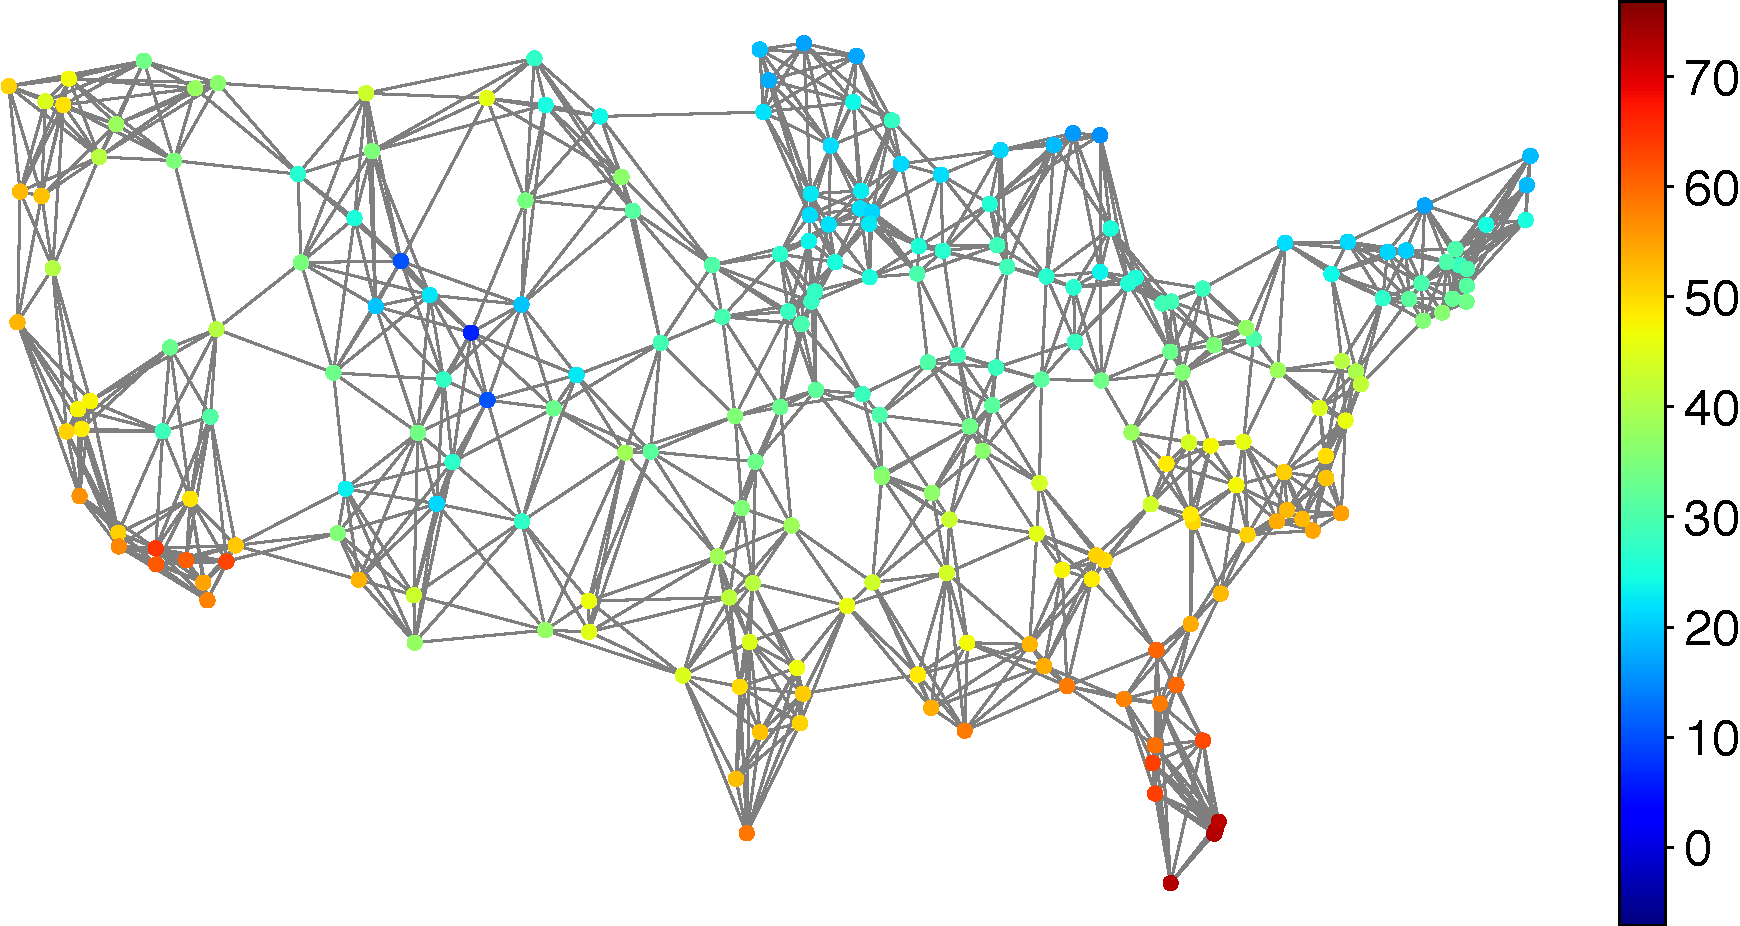
\includegraphics[width=\linewidth]{Figures/GNorm_estacoes_temperatura.pdf}
	\caption{Graph of a network formed by $230$ weather stations measuring the temperature across the United States. The snapshot of all measurements taken on February $1^{\text{st}}$, 2003 is the corresponding graph signal.}%
	\label{fig:usa00}%
	\vspace{0.14cm}
\end{figure}

\begin{figure}[ht!]%
	\centering
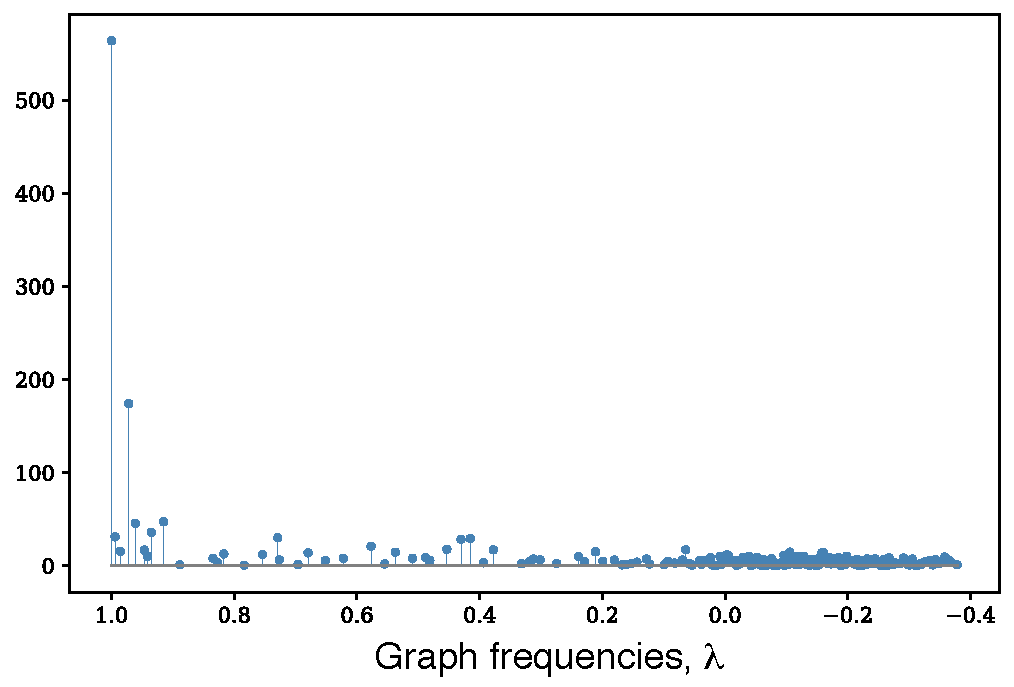
\includegraphics[width=0.88\linewidth]{Figures/GNorm_estacoes_GFT_Temperatura.pdf}%\vspace{-0.1cm}
	\caption{Magnitude of the graph Fourier transform of the signal in Fig~\ref{fig:usa00}. The graph frequencies correspond to the eigenvalues of $\mathbf{A}$; low (resp. high) graph frequencies are associated with higher (resp. lower) eigenvalues.}%
	\label{fig:usa01}%
	%\vspace{-0.2cm}
\end{figure}

\begin{figure}[ht!]
	\centering
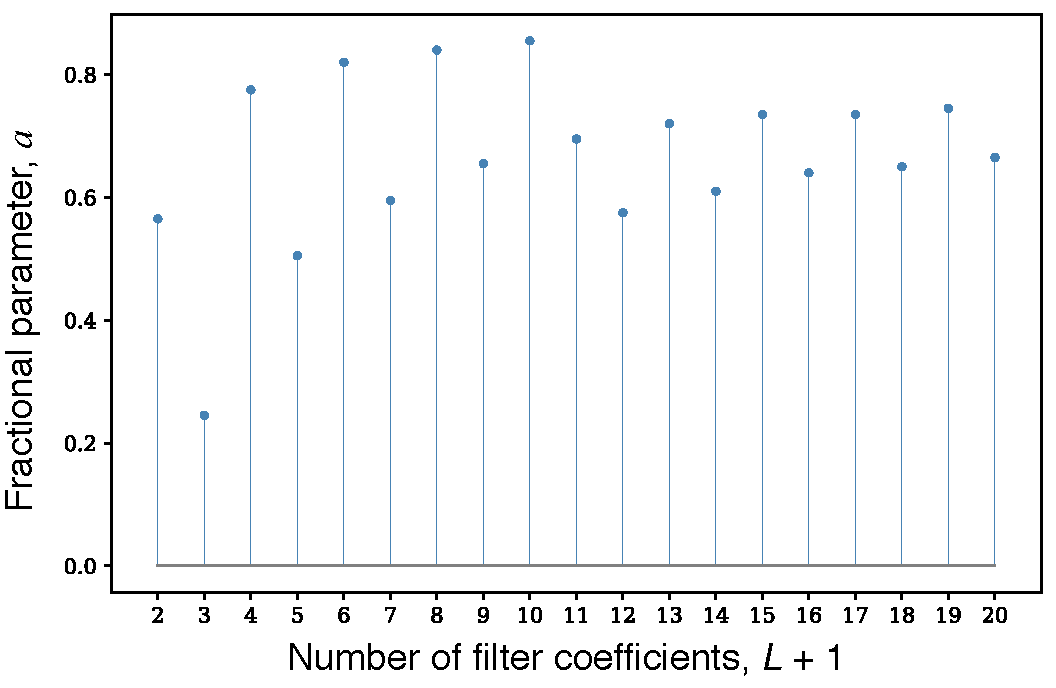
\includegraphics[width=0.9\linewidth]{Figures/ERROR_ordens_fracionarias.pdf}
	\caption{Fractional parameters providing the minimum approximation errors, for different values of $L$, between the ideal LPF and the filter designed by using the fractional graph shift operator $\mathbf{A}^a$.}%
	\label{fig:usa02}%
	%\vspace{-0.5cm}
\end{figure}

We then use the strategy explained in Subsection~\ref{subsec:lsi} to design a filter that approximates an ideal low-pass filter with $\lambda_{i_\text{cut}}=0.2$. In this case, $i_\text{cut}=39$ so that the $40$ lowest graph frequencies are (ideally) preserved after the signal is filtered. We considered approximations with $L$ ranging from $1$ to $19$, that is, filters with $2$ to $20$ coefficients. For each of these values, we varied the fractional parameter $a$ from $0$ to $1$ and, in~(\ref{eq:siseq2}), after replacing $\lambda_i$ with $\lambda_i^a$, $i=0,1,\ldots,N-1$, and solving~(\ref{eq:opt})\footnote{The optimization problem~\ref{eq:opt} has been solved using the Linear Algebra module \emph{linalg} for Scipy, a free and open-source Python library used for scientific and technical computing. In all experiments performed, the least mean squares algorithm converged and the time required for this was negligible, considering the addressed application scenario.}, we registered the value of $a$ providing the minimum error between the designed filter and the ideal filter. At the end of this procedure, the graph shown in Fig.~\ref{fig:usa02} was produced. Observing the figure, we verify that, for any value of $L$, the best approximation is provided when $a\neq1$. This is enough to conclude that, for the graph considered in the example, the use of a fractional version $\mathbf{A}^a$, $a\neq 1$, of $\mathbf{A}$ always provides a better result than the one obtained with the non-fractional matrix. A visual comparison between these alternatives can be performed from Fig.~\ref{fig:usa03}, where we show the (minimum) errors we have just referred to together with the errors when the original (non-fractional) matrix $\mathbf{A}$ is employed.

In Fig.~\ref{fig:usa04}, we can observe the ideal filter response superimposed on the responses obtained when $\mathbf{A}$ and $\mathbf{A}^a$ are used to design a filter with $L+1=10$ coefficients. In this case, the fractional parameter providing the minimum error is $a=0.855$. In the figure, we notice that the filter designed with $\mathbf{A}^a$ has fluctuations that deviate less from the ideal filter, when compared to those related to the filter designed using $\mathbf{A}$. This can be observed mainly in the passband and constitutes a visual result coherent with the obtained approximation errors. Graphs with similar behaviour are obtained for other values $L$.

\begin{figure}[t!]
	\centering
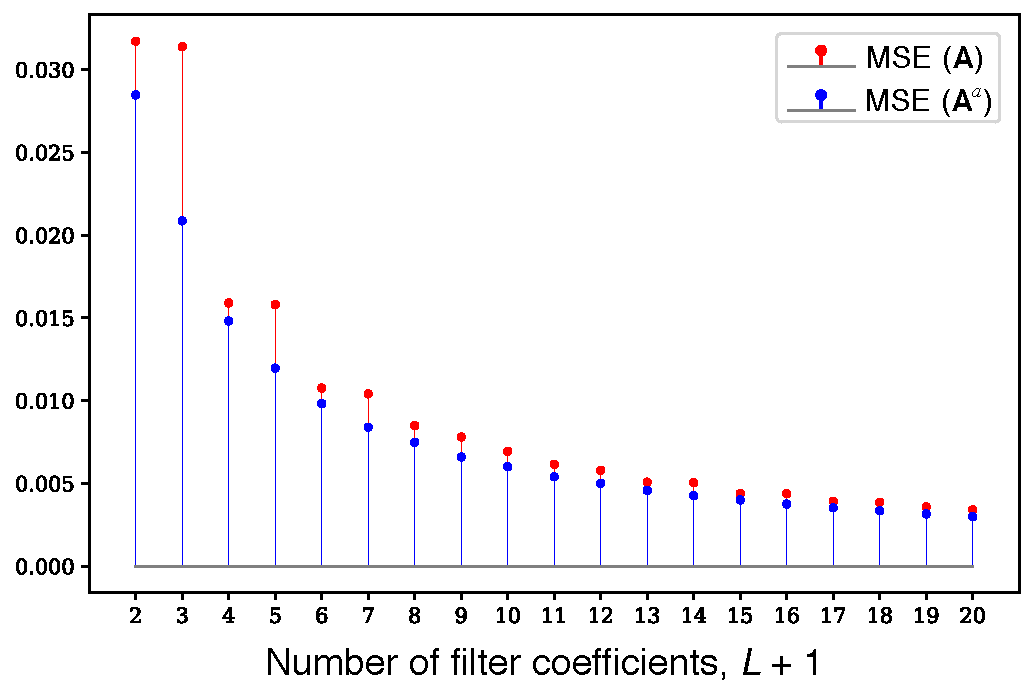
\includegraphics[width=0.9\linewidth]{Figures/ERROR_mse_min.pdf}
	\caption{Minimum approximation (mean squared) errors, for different values of $L$, between the ideal LPF and the filters designed by using the fractional graph shift operator $\mathbf{A}^a$ and the non-fractional operator $\mathbf{A}$.}%
	\label{fig:usa03}%
	%\vspace{-0.2cm}
\end{figure}

\begin{figure}[t!]
	\centering
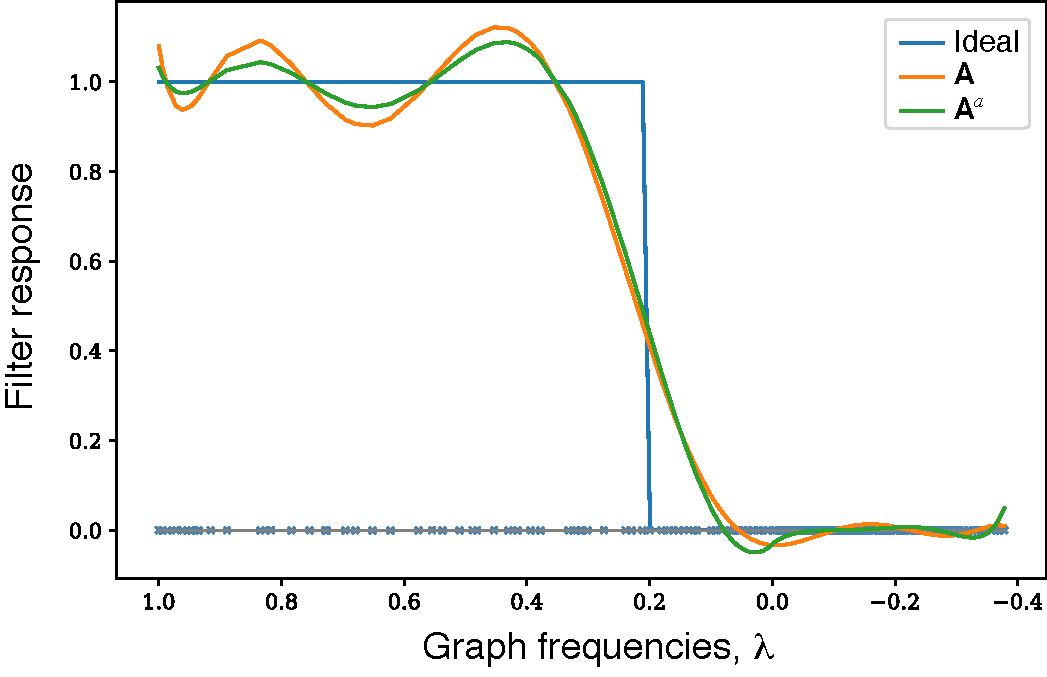
\includegraphics[width=0.88\linewidth]{Figures/ERROR_estacoes_resposta_grau10.pdf}%\vspace{-0.4cm}
	\caption{Ideal filter response superimposed on the responses obtained when $\mathbf{A}$ and $\mathbf{A}^a$, $a=0.855$, are used to design a filter with $L+1=10$ coefficients.}
	\label{fig:usa04}%
	%\vspace{-0.2cm}
\end{figure}

\subsection{Example: Noise Removal}\label{subsec:lsi02}
In this example, we start from the same graph signal considered in Subsection~\ref{subsec:lsi01}. We add to the samples of the referred signal random uniformly-distributed values whose amplitude corresponds to a percentage of the range of the signal itself. Such a synthetic noise addition is intended to simulate what happens in many practical scenarios, in which measurements performed on a sensor network are subject to different sources of distortion. The resulting noisy signal is then filtered by using the filters shown in Fig.~\ref{fig:usa04}, as an attempt to reduce the influence of the noise and recover the original signal.

In our experiment, we varied the aforementioned percentage from $1\%$ to $50\%$ and, for each of these values, we generated $100$ noisy signals. We then filtered such signals and compared the resulting signals with the original (non-noisy) signal by the computation of mean-squared errors. The results, which can be viewed in Fig.~\ref{fig:usa05}, show that the filter designed using $\mathbf{A}^{0.855}$ allows to recover the signal with average reconstruction error always smaller than that related to the filter designed using $\mathbf{A}$. \textcolor{black}{In this context, it is relevant to remark that the (best) fractional parameter $a=0.855$ has been found using the strategy described in the second paragraph of Subsection~\ref{subsec:lsi01}, which depends on the error between the designed filter and the ideal filter only. Therefore, the referred choice does not require us to know the original signal, which is not available in the real-world.} This illustrates the potential gain that can be achieved, in this application scenario, when considering the possibility of fractionalization of the graph shift operator.

\textcolor{black}{Finally, it is also interesting to mention that only one or a few nodes could have had their measurements corrupted by noise or changed due to other factors; this would represent a scenario in which certain sensors would be malfunctioning. In order to obtain some preliminary results taking into account the above described assumption, we carried out additional simulations. To be more specific, we basically repeated our previous tests, but assuming that only a number from $1$ to $12$ nodes had their values nullified or increased by $20$ times. We then performed a low-pass filtering, expecting that the high-frequency component associated with the referred measurement changes would be attenuated and that the smooth behavior of the signal would be recovered. In general, the results obtained using the proposed fractional operator were better or at least equivalent to those obtained with the corresponding ordinary operator. In a future work, we intend to address this issue in more detail.}

\begin{figure}[t!]
	\centering
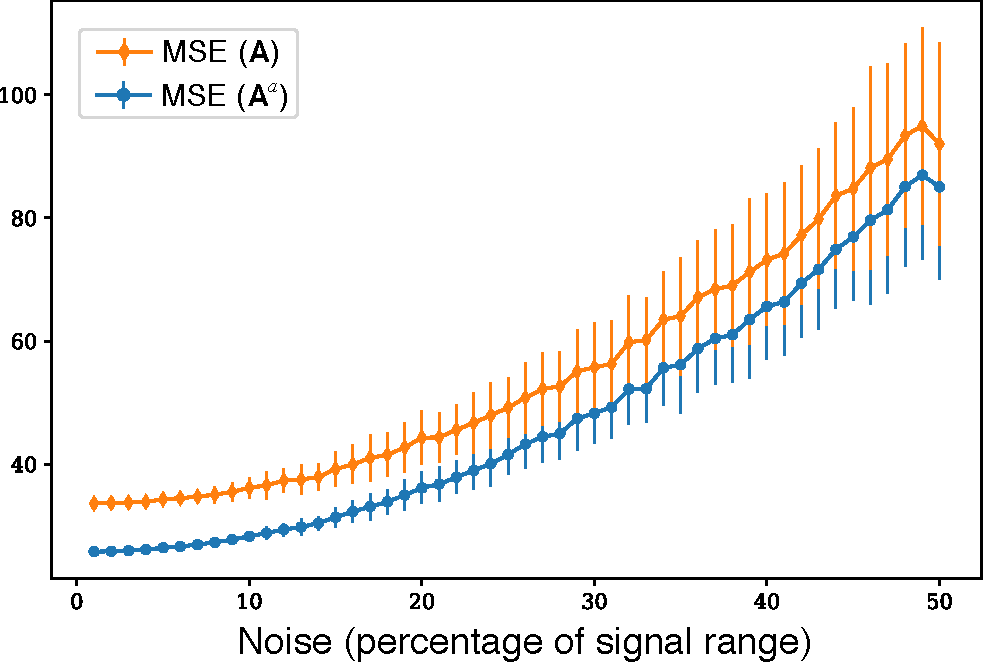
\includegraphics[width=0.95\linewidth]{Figures/ERROR_errobar_filtrados.pdf}
	\caption{Reconstruction (mean squared) errors after a noise removal procedure is performed by using graph filters with $L+1=10$ coefficients and designed from $\mathbf{A}$ and $\mathbf{A}^a$, $a=0.855$.}%
	\label{fig:usa05}%
	\vspace{-0.1cm}
\end{figure}

\section{Concluding Remarks}\label{sec:conc}
In this paper, we have investigated the fractional shift of graph signals. The key-point for our developments is the fact that, in the GSP theory, the unit shift is defined from the adjacency matrix of a graph. Interpreting the fractional shift as a filtering operation, we demonstrated that, for ring graphs, its application produces the expected effect of approximating the classical ideal interpolating filter, exhibiting satisfactory results for band-limited signals. We have also shown that the referred fractional operator can be implemented as an LSI graph filter for arbitrary graphs and developed real-world examples that illustrated the benefits of using $\mathbf{A}^a$ to design graph filters for noise removal. Our current investigations include the study of the fractionalization of other operators on graphs (e.g., graph Fourier transform and Laplacian), other types of generalization for the same operators and further applications of the fractional graph shift. \textcolor{black}{In particular, we have been studying the use of $\mathbf{A}^a$ to design filters for anomaly detection on graphs (malfunctioning nodes in a sensor network, for instance) and evaluating the feasibility of introducing a kind of generalized degree index, so that long range interactions can be considered.}


\chapter{The fractional quaternion discrete Fourier transform and its applications}

Linear discrete transforms are building blocks for a multitude of techniques in the field of signal processing, being almost as important as they are diverse. Among the factors which distinguish one from the others, there is the algebraic structure over which they are defined, e.~g. a finite field and its extensions (such as in number-theoretic \cite{blahut2010fast,pedrouzo2017number,chandra2014exact,lima2013} and arithmetic \cite{knockaert1994generalized, rajapaksha2014vlsi} transforms), or the real and complex fields (as in the usual discrete Fourier transform). As the algebra is extended (for instance, from $ \mathbb{R} $ to $ \mathbb{C} $), it is possible to encode more information into each signal sample. Such was the motivation behind Sangwine's definition \cite{sangwine1996fourier} of discrete two-dimensional quaternion transforms, based on their continuous counterparts previously defined by Ell \cite{ell1993quaternion}: to apply these four-dimensional numbers --- the quaternions, an extension of the complex field --- to color image processing. Since then, quaternion transforms have been useful not only to image processing \cite{ell2007hypercomplex,chen2018quaternion,li2013quaternion,evans2000hypercomplex,silva2018}, but also to other fields, such as bivariate signal analysis \cite{flamant2017spectral,flamant2017time,flamant2018complete}.

Fractional transforms are yet another class of tools of great use. The fractional Fourier transform has been applied to time-frequency analysis, compression, digital watermarking, filtering, encryption, let alone its utility in Optics \cite{bultheel2002shattered,figueiredo2018}. Regarding quaternion transforms, a couple of competent works have already addressed their fractionalization \cite{guanlei2008fractional, wei2013different, roopkumar2016quaternionic} and some applications have been proposed \cite{chen2018quaternion}. However, the authors are not aware of papers approaching fractional quaternion discrete transforms from an eigenstructure analysis point of view. This reasoning may unfold new theoretical insights and implementation techniques, and such is the motivation for this work.

In this paper, the eigenstructure of the quaternion discrete Fourier transform (QDFT) matrix is investigated and shown to be closely related to that of the unitary discrete Fourier transform (DFT). This result offers an approach for defining the fractional version of the QDFT (referred to as FrQDFT). Following the central goal of defining the transform through eigendecomposition theory, a generalization is proposed in the form of a multiple-parameter fractional quaternion discrete Fourier transform (MFrQDFT). For illustrative purposes, this work proposes and briefly explores an encryption scheme for color images with opacity layer, fully harnessing the holistic processing of 4-layered 2D signals through the MFrQDFT.

The proposed method for image encryption fits in the class of schemes that use linear transforms alongside non-linear blocks \cite{hsue2018enhancing}, to implement confusion and diffusion. The currently available methods in the state-of-the-art literature respond to a diverse range of needs, as fast implementation through parallel computing \cite{wang2019fast}, increased safety and robustness by using matrix semi-tensor product \cite{wang2020image} or one-time keys \cite{liu2010}, just to name a few examples. The main scope of this paper is not the encryption scheme \textit{per se}, but rather the FrQDFT eigenscructure and the MFrQDFT definition, the latter having the image encryption as a framework to showcase some of its possibilities. Nevertheless, the proposed encryption algorithm is described and evaluated to some extent. Although being an illustrative scenario, it stands on tools adopted currently by the literature. For example, the chosen method for key generation involved the use of chaotic maps, known to help achieving high bit sensibility and large key space. It follows works such as the one by Liu and Wang \cite{liu2011color}, which proposed a color image encryption scheme using two chaotic maps and one-time keying, aiming to achieve large key space and cycle lengths. Another work by Liu and Wang \cite{liu2012} employed a piecewise linear chaotic map and DNA encoding for ensuring the initial conditions of the encryption change according to the image, whereas Wang \textit{et al.} \cite{wang2010chaotic} used a Lorentz chaotic map and a perceptron model applied to image encryption. The proposed scheme uses a chaotic tent map to generate a pseudo-random sequence, from which the secret parameters are extracted.


This paper is structured as follows. Section \ref{sec:autoestrutura} presents the usual definition of the QDFT and proves the central theorem of this work, regarding how the DFT and QDFT share symmetric eigenvectors; it closes with comments on the quaternion representation of color images with opacity layer. Section \ref{sec:FrQDFT} discusses the fractionalization of the QDFT from an eigenstructure point of view and demonstrates some properties purely based on matrix algebra. Section \ref{sec:multi} proposes a multiple-parameter extension of the fractional transform and presents an application involving encryption of color images with opacity layer. The main results are summarized in Section \ref{sec:conclusao}, and the paper closes with a brief Appendix on basic quaternion algebra.


\section{Eigenstructure of the QDFT}
\label{sec:autoestrutura}
Quaternion Fourier transforms (QFT) have received quite a few definitions. Some are one-dimensional \cite{flamant2017spectral}, while others are intrinsically two-dimensional \cite{guanlei2008fractional}; the latter group can yet be divided into those having kernels oriented towards generic pure unit quaternions\footnote{The reader may refer to the Appendix to a brief revision on the set of quaternion numbers $ \mathbb{H} $, their algebra and terminology.}, and those using canonic imaginary units, such as $ \qi $ and $ \qj $. The 2D-transformed signals may be placed \textit{between} the two kernels or beside them. In fact, Ell \cite[sec. 3.2]{ell2014quaternion} lists 8 possibilities for the 2D-QFTs.

In this paper, we use the QDFT of axis $ \qmu $ as defined in \cite[sec. 3.3.1]{ell2014quaternion}. Let $ \qmu $ be a unit pure quaternion. Then, the $ m$-th entry of the QDFT of vector $ \mathbf{v} $ is

\begin{equation}
\label{eq:QDFT_fwd}
\!\widehat{v}_m \!=\! \text{QDFT}\{ \mathbf{v} \}_m \!\overset{\Delta}{=}\! \frac{1}{\sqrt{N}} \!\sum_{n=0}^{N-1}  \exp \left( -\qmu \frac{2\pi}{N} nm \right) v_n \!\in\! \mathbb{C}_{\qmu},\!
\end{equation}
in which $ \mathbb{C}_{\qmu} $ denotes the set of numbers $ a + \qmu b $, $ a,b \in \mathbb{R} $, isomorphic to the complex set. It matters to notice that, due to the lack of commutativity in quaternion multiplication, the position of the kernel relative to the signal in (\ref{eq:QDFT_fwd}) is relevant and must be kept consistent along all computations. Hence, the inverse transformation must be computed with the kernel on the same relative position,
\begin{equation}
\label{eq:QDFT_inv}
v_n = \text{QDFT}^{-1}\{ \widehat{\mathbf{v}} \}_n = \frac{1}{\sqrt{N}}\sum_{m=0}^{N-1}  \exp \left( \qmu \frac{2\pi}{N} nm \right) \widehat{v}_m.
\end{equation}

The synthesis and analysis equations may be written in matrix form as
\begin{equation}
\label{eq:QDFT}
\widehat{\mathbf{v}} = \text{QDFT}\{ \mathbf{v} \} = \mathbf{F} \mathbf{v},
\end{equation}
\begin{equation}
\label{eq:QDFT_mtx_inv}
\mathbf{v} = \text{QDFT}^{-1}\{ \widehat{\mathbf{v}} \} = \mathbf{F}^{-1} \widehat{\mathbf{v}},
\end{equation}
where $ \mathbf{F} $ is the unitary QDFT matrix, with entries $ \{\mathbf{F}\}_{n,m} = \sqrt{N}^{-1} \exp \left( -\qmu \frac{2\pi}{N} nm \right)$. Since $ \exp \left( -\qmu \frac{2\pi}{N} \right) $ is an $ N $-th root of unity, such as $ \exp \left( -\qi \frac{2\pi}{N} \right) $, it follows that $ \mathbf{F} $ shares many properties of the DFT matrix, such as invertibility (simple calculations show that $ \mathbf{F}^{-1} = \mathbf{F}^{H} $), what guarantees validity of the inversion formulae in (\ref{eq:QDFT_inv}) and (\ref{eq:QDFT_mtx_inv}).

The two-dimensional QDFT can be defined in a similar fashion, although more options regarding kernel positioning are available, since for any pure quaternions $ \qmu \neq \qnu $, one may verify that generally $ e^{\qnu \alpha} e^{\qmu \beta} \neq e^{\qnu \alpha + \qmu \beta} $. Ell and Sangwine \cite{ell2014quaternion} presented the \textit{eight} distinct ways of building a 2D-QFT, which translate directly into options for 2D-QDFT. One of such possibilities is to transform the quaternion-valued matrix $ \mathbf{X} \in \mathbb{H}^{N\times M}$ according to the equation
\begin{equation}
\label{eq:2DQDFT-01}
\hat{X}_{u,k} = 
\text{2D-QDFT}\{ \mathbf{X} \}_{u,k} \!\overset{\Delta}{=}\! \frac{1}{\sqrt{MN}} \!\sum_{n=0}^{N-1} \sum_{m=0}^{M-1}  \exp \left( -\qmu \frac{2\pi}{N} nu \right) X_{n,m} \exp \left( -\qnu \frac{2\pi}{M} mk \right).
\end{equation}
This formulation of the 2D-QDFT translates into the following matrix equation,
\begin{equation}
\label{eq:2DQDFT-02}
\hat{\mathbf{X}} = \mathbf{F}^{(\qmu)} \mathbf{X} \mathbf{F}^{(\qnu)},
\end{equation}
where the Fourier matrices are similar to the one used in (\ref{eq:QDFT}), except from the pure quaternion which serves as transform axis (shown in the parenthesis). This is a consequence of the \textit{separability} of the 2D-QDFT, by which this transform may be conceived as the successive application of two 1D-QDFTs: once in the rows of $ \mathbf{X} $, once in the columns. Therefore, some results and properties derived for the 1D-QDFT may naturally extend to the two-dimensional case.

Although the quaternion eigenvalue problem has been extensively studied and proven to be challenging \cite{de2002quaternionic,flaut2002eigenvalues,jiang2004algorithm,farid2011eigenvalues}, the investigation of the eigenstructure of matrix $ \mathbf{F} $ may benefit from the similarities between the QDFT and the DFT. As a result of Theorem \ref{th:01}, one is able to deduce the QDFT eigenstructure out of even and odd DFT eigenvectors, by using a variation of Pei's reasoning regarding the 2D-QDFT \cite{pei2010eigenfunctions}.

\begin{theorem}
\label{th:01}
Let $ \mathbf{v} $ be an eigenvector of the unitary DFT with eigenvalue $ \lambda $.
\begin{itemize}
\item[(a)] If $ \mathbf{v} $ has even symmetry (in which case $ \lambda = \pm 1 $), then it is also an eigenvector of the QDFT with eigenvalue $ \lambda $.
\item[(b)] If $ \mathbf{v} $ has odd symmetry (in which case $ \lambda = \pm \qi $), then it is also an eigenvector of the QDFT (of axis, let us say, $ \qmu $) with eigenvalue $ -\lambda \qi \qmu$, i.~e. $ \pm \qmu $.
\end{itemize}
\end{theorem}

\begin{proof}
\begin{itemize}
\item[(a)] If $ \mathbf{v} $ has even symmetry, i.~e. $ v_n = v_{N-n} $ for $ n=1,\dots,N-1 $, then
\begin{equation}
%\label{key}
\sum_{n=0}^{N-1} v_n \sin \frac{2\pi}{N} nm = 0,
\end{equation}
therefore,
\newcommand{\correctinghspace}{-1.8cm}
\begin{equation}
%\small
\label{eq:15}
\begin{aligned}
\sqrt{N} \text{QDFT}\{ \mathbf{v} \}_m &= \sum_{n=0}^{N-1} v_n e^{-\qmu \frac{2\pi}{n} nm} \\
&\hspace{\correctinghspace}
=\sum_{n=0}^{N-1} v_n \left( \cos \frac{2\pi}{n} nm - \qmu \sin \frac{2\pi}{n} nm \right) \\
&\hspace{\correctinghspace}
= \left( \sum_{n=0}^{N-1} v_n \cos \frac{2\pi}{n} nm \right) - \underbrace{\left(  \sum_{n=0}^{N-1} v_n \sin \frac{2\pi}{n} nm \right)}_{=0} \qmu \\
&\hspace{\correctinghspace}
= \left( \sum_{n=0}^{N-1} v_n \cos \frac{2\pi}{n} nm \right) - \underbrace{\left(  \sum_{n=0}^{N-1} v_n \sin \frac{2\pi}{n} nm \right)}_{=0} \qi \\
&\hspace{\correctinghspace}
= \sqrt{N} \text{DFT}\{ \mathbf{v} \}_m = \sqrt{N} \lambda v_m \\
&\hspace{\correctinghspace}
\Rightarrow \text{QDFT}\{ \mathbf{v} \} = \lambda \mathbf{v}.
\end{aligned}
\end{equation}
\item[(b)] If $ \mathbf{v} $ has odd symmetry, i.~e. $ v_n = -v_{N-n} $ for $ n=1,\dots,N-1 $ and $ v_0 = 0 $, then
\begin{equation}
%\label{key}
\sum_{n=0}^{N-1} v_n \cos \frac{2\pi}{N} nm = 0,
\end{equation}
hence,
\begin{equation}
\small
\label{eq:17}
\begin{aligned}
\sqrt{N} \text{QDFT}\{ \mathbf{v} \}_m &= \sum_{n=0}^{N-1} v_n e^{-\qmu \frac{2\pi}{n} nm}\\
&\hspace{\correctinghspace}
=
\sum_{n=0}^{N-1} v_n \left( \cos \frac{2\pi}{n} nm - \qmu \sin \frac{2\pi}{n} nm \right) \\
&\hspace{\correctinghspace}
= {\underbrace{\left( \sum_{n=0}^{N-1} v_n \cos \frac{2\pi}{n} nm \right)}_{=0} - \left(  \sum_{n=0}^{N-1} v_n \sin \frac{2\pi}{n} nm \right) \qmu }\\
&\hspace{\correctinghspace}
= - \left(  \sum_{n=0}^{N-1} v_n \sin \frac{2\pi}{n} nm \right) \qmu.
\end{aligned}
\end{equation}

But, from the odd symmetry assumption,
\begin{equation}
%\label{key}
\begin{aligned}
\sqrt{N}\lambda v_m = \sqrt{N}\text{DFT}\{ \mathbf{v} \}_m &= \sum_{n=0}^{N-1} v_n e^{-\qi \frac{2\pi}{n} nm}= - \left(  \sum_{n=0}^{N-1} v_n \sin \frac{2\pi}{n} nm \right) \qi,
\end{aligned}
\end{equation}
therefore (remember that $ \lambda $ and $ v_m $ commute)
\begin{equation}
\label{eq:19}
\sum_{n=0}^{N-1} v_n \sin \frac{2\pi}{n} nm = \sqrt{N}v_m \lambda \qi.
\end{equation}
From (\ref{eq:17}) and (\ref{eq:19}),
\begin{equation}
\label{eq:20}
\begin{aligned}
\sqrt{N}\text{QDFT}\{ \mathbf{v} \}_m &=  -\sqrt{N}\text{DFT} \{ \mathbf{v} \}_m \qi \qmu \\
&\hspace{\correctinghspace}
= -\sqrt{N}v_m \lambda \qi \qmu \\
&\hspace{\correctinghspace}
\Rightarrow \text{QDFT}\{ \mathbf{v} \} = -\lambda \qi \qmu \mathbf{v}.
\end{aligned}
\end{equation}
\end{itemize}
\end{proof}

The results of Theorem \ref{th:01} are summarized in Table \ref{tab:01}.
This analysis can immediately be extended to the two-dimensional case if one considers the separability of the 2D-QDFT, mentioned after (\ref{eq:2DQDFT-02}). If $ (\mathbf{e}^{(\qmu)}, \lambda_{\qmu}) $ and $ (\mathbf{e}^{(\qnu)}, \lambda_{\qnu}) $ are (column-)eigenvector-eigenvalue pairs of the matrices $ \mathbf{F}^{(\qmu)} $ and $ \mathbf{F}^{(\qnu)} $, respectively, then the 2D signal $ \mathbf{e}^{(\qmu)} \mathbf{e}^{(\qnu)^T}  $ is a 2D-QDFT eigenvector with eigenvalue $ \lambda_{\qmu} \lambda_{\qnu} $ \cite{candan2011}. Therefore, this 2D-QDFT has eight (possibly) distinct eigenvalues: $ \pm 1, \pm \qmu, \pm \qnu, \pm \qmu \qnu $.

\begin{table}[b!]
\center
\captionof{table}{DFT and QDFT eigenvectors.}
\label{tab:01}
\begin{tabular}{ccc}
\toprule
\shortstack{Eigenvector\\ symmetry} & \shortstack{Eigenvalue\\(DFT)} & \shortstack{Eigenvalue\\(QDFT)} \\
\midrule
Even & $ \pm 1 $ & $ \pm 1 $ \\
Odd & $ \pm \qi $ & $ - (\pm \qi) \qi \qmu = \pm \qmu $\\
\bottomrule
\end{tabular}
\end{table}

\subsection{2D-QDFT and color images with opacity layer}
\label{subsec:2D_QDFT}
The 2D-QDFT has been commonly used to process color images, which are represented as matrices of pure quaternions \cite{lu20072d,ell2006hypercomplex,chen2018multiple}. In this representation, each color channel of a certain pixel corresponds to an imaginary component of the pure quaternion. Although this mapping is useful and adequate, it neglects the quaternion scalar part (always set to zero), causing a difference in dimensionality between input and output of the 2D-QDFT: while the image is a 2D signal with three-dimensional components, its spectrum has four-dimensional entries. It surely is not a problem \textit{per se}, rather is an inconvenience, also found when processing real signals with the DFT.

An application free from this inconvenience is the analysis of color images with opacity (or alpha) layer, as in files in PNG format (portable network graphics). In this case, each pixel $ (R,G,B,\alpha) $ is mapped into $ q = \alpha + R \qi + G \qj + B \qk $, forming the quaternion-valued matrix $ \mathbf{X} $. Let us compute the 2D-QDFT by separately transforming the rows and columns using (\ref{eq:2DQDFT-02}), with the same transform axis on both sides,
\begin{equation}
\label{eq:2DQDFT}
\text{2D-QDFT}\{\mathbf{X} \} = \mathbf{F} \mathbf{X} \mathbf{F}^T.
\end{equation}

One should notice that the transformation in (\ref{eq:2DQDFT}) does \textit{not} consist on the successive application of the \textit{same} QDFT to the rows and columns of matrix $ \mathbf{X} $. Due to the non-commutative nature of quaternion multiplication, as it was previously mentioned, different transforms are obtained when choosing between left- or right-multiplications, even though the transform axis is kept unchanged. The operation in (\ref{eq:2DQDFT}) performs a \textit{left} QDFT on the columns and a \textit{right} QDFT on the rows, as it is clear from (\ref{eq:2DQDFT-01}). A 2D-QDFT consisting of the \textit{same} transformation applied in both dimensions must use multiplications with the same orientation, e.~g.
\begin{equation}
\label{eq:2DQDFTv2}
\mathbf{F} \left( \mathbf{F}\mathbf{X}^T \right)^T.
\end{equation}

Fig. \ref{fig:2D_QDFTv1} shows the QDFT -- according to (\ref{eq:2DQDFT}) -- of Fig. \ref{fig:dice}, as another PNG image. As an illustration of the difference in using (\ref{eq:2DQDFT}) or (\ref{eq:2DQDFTv2}), caused by the lack of commutativity in quaternion multiplication, the mean squared error (MSE) between the two spectra was computed. The result was approximately 1070. % Cálculo feito com o script trying_separable_2DQDFT.py


%{\color{red}(Mantemos isso?) \'E curioso observar que, ao processar imagens em PNG utilizando a 2D-QDFT, tanto o sinal (imagem) de entrada como o de sa\'ida s\~ao compostos por quaternions (geralmente) n\~ao-puros, o que permite usar a mesma representa\c c\~ao no dom\'inio do sinal e da transformada. Ao usar a 2D-DFT para processar imagens em escala de cinza, ou a 2D-QDFT para imagens em RGB, o dom\'inio espectral difere daquele do sinal original.}

\begin{figure}
\centering
\subfloat[\label{fig:2D_QDFTv1}]{
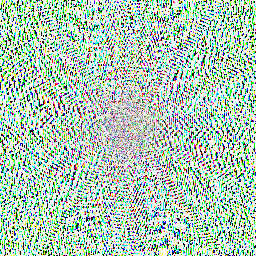
\includegraphics[width=0.3\linewidth]{Figures/2D_QDFTv1.png}
}~
\subfloat[\label{fig:2D_QDFTv2}]{
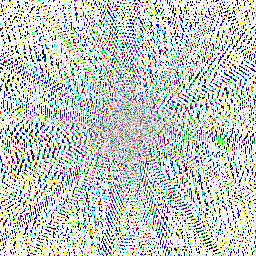
\includegraphics[width=0.3\linewidth]{Figures/2D_QDFTv2.png}
}
\caption{(a) 2D-QDFT of the PNG image in Fig. \ref{fig:dice}, according to (\ref{eq:2DQDFT}), with axis $ \qmu = \frac{1}{\sqrt{3}}(\qi + \qj + \qk) $. (b) 2D-QDFT of the same image, same transform axis, following the approach in (\ref{eq:2DQDFTv2}).}
\label{fig:QDFT}
\end{figure}

\section{Fractional Quaternion Discrete Fourier Transform}
\label{sec:FrQDFT}
%Incluir defini\c{c}\~ao da transformada, a qual sugiro que seja identificada pelo acr\^onimo FrQDFT (do ingl\^es \emph{fractional quaternions discrete Fourier transform}), empregando o conte\'udo desenvolvido na se\c{c}\~ao anterior e abordar as principais propriedades.

The proposed fractionalization method explores the eigenvector sharing between the DFT and the QDFT: as long as one possesses an orthogonal eigenvector matrix $ \mathbf{E} $ for the DFT, it can be used for the QDFT matrix diagonalization and its subsequent fractionalization. For instance, the eigendecomposition of the DFT matrix allows to find its fractional counterpart by raising each eigenvalue to a non-integer parameter $ a $, i.~e.

\begin{equation}
\label{eq:FrDFT}
\mathbf{F}_{\text{DFT}}^a = \mathbf{E} \mathbf{\Lambda}^a \mathbf{E}^T,
\end{equation}
where $ \mathbf{\Lambda} $ is the diagonal matrix containing the DFT eigenvalues.

Oliveira and Lima \cite{de2017discrete} stress that a FrDFT expressed as in (\ref{eq:FrDFT}) will numerically approximate its continuous version if and only if the columns of $ \mathbf{E} $ approximate samples of continuous Hermite-Gaussian functions. In \cite{de2017discrete}, the authors present two methods to generate such an orthogonal eigenbasis, one of which (the generating matrix method) is the one adopted in this work.

\begin{figure*}
\centering
\subfloat[\label{fig:dice}]{
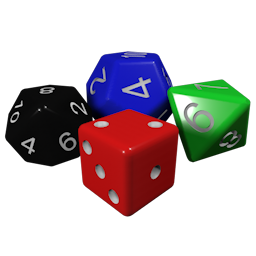
\includegraphics[width=0.25\linewidth]{Figures/dice_256x256.png}
}~
\subfloat[]{
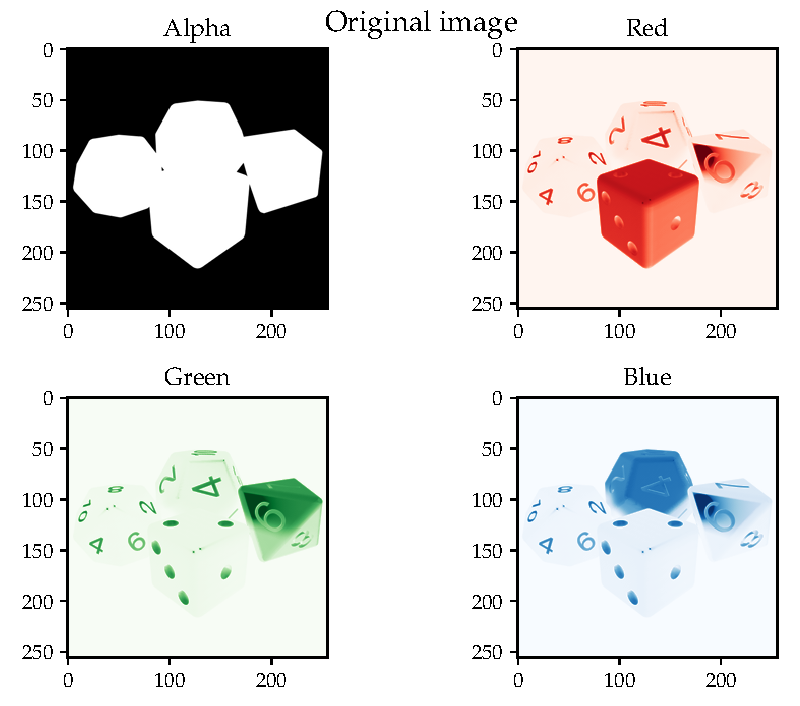
\includegraphics[width=0.35\linewidth]{Figures/dice_256x256_layers.pdf}
}~
\subfloat[]{
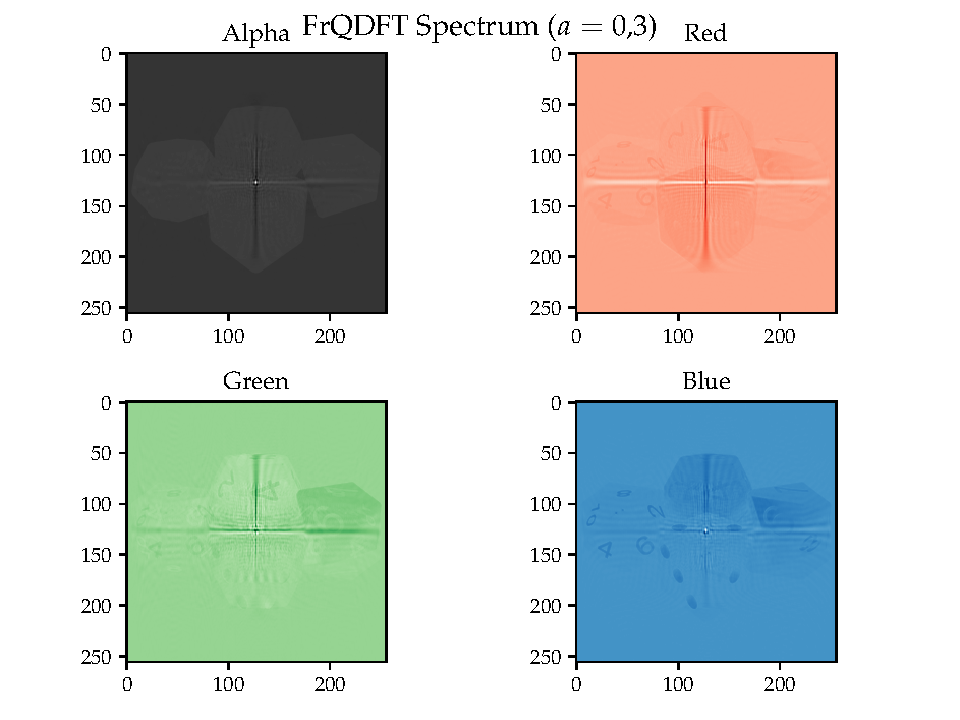
\includegraphics[width=0.35\linewidth]{Figures/dice_256x256_layers_frqdft.pdf}
}~
\caption{(a) Test PNG image. Visualization of each layer in the (b) test image and (c) in its FrQDFT spectrum, computed with transform axis $ \qmu = \frac{1}{\sqrt{3}}(\qi + \qj + \qk) $ e $ a=0{.}3 $.}
\end{figure*}

Once one is able to compute an orthogonal eigenbasis $ \mathbf{E} $ containing Hermite-Gaussian-like DFT eigenvectors, for instance by means of the generating matrix method, Theorem \ref{th:01} assures that matrix $ \mathbf{E} $ is also an eigenvector matrix for the QDFT. As a consequence, the transform matrix $ \mathbf{F} $ may be decomposed and written as
\begin{equation}
\label{eq:QDFTmtx}
\mathbf{F} = \mathbf{E} \mathbf{\Gamma} \mathbf{E}^T,
\end{equation}
in which the diagonal matrix $ \mathbf{\Gamma} $ is obtained by replacing $ \qi $ with $ \qmu $ in $ \mathbf{\Lambda} $ (Table \ref{tab:01}). Therefore, the \textit{fractional} quaternion Fourier transform, or simply FrQDFT, is obtained by raising each eigenvalue in $ \mathbf{\Gamma} $ to a so-called fractional order $ a \in \mathbb{R} $, so that
\begin{equation}
\label{eq:QDFTmtxa2}
\text{FrQDFT}_a\{ \mathbf{v} \} \overset{\Delta}{=} \mathbf{F}^a \mathbf{v},
\end{equation}
%\ref{eq:QDFTmtx}
where
\begin{equation}
\label{eq:QDFTmtxa}
\mathbf{F}^a = \mathbf{E} \mathbf{\Gamma}^a \mathbf{E}^T.
\end{equation}

The FrQDFT, as defined in (\ref{eq:QDFTmtxa2}) and (\ref{eq:QDFTmtxa}), possesses all the classical properties of a fractional Fourier transform:

\begin{itemize}
\item \textit{Reduction to the ordinary quaternion transform}: if $ a=1 $, then the synthesis equation in (\ref{eq:QDFTmtxa2}) equals (\ref{eq:QDFT}), coinciding with the QDFT. The proof is imediate.

\item \textit{Reduction to the identity}: if $ a=0 $, the FrQDFT reduces to the identity operator, represented as $ \mathbb{I} $.

\begin{proof}
From the orthogonality of the eigenvector matrix $ \mathbf{E} $,
\begin{equation}
%\label{key}
\mathbf{F}^0 = \mathbf{E} \mathbf{\Gamma}^0 \mathbf{E}^T = \mathbf{E} \mathbf{E}^T = \mathbb{I}.
\end{equation}
\end{proof}

\item \textit{Index addititivy}: applying the FrQDFT twice, using $ a $ and $ b $ as fractional orders, equals applying a single FrQDFT with fractional order $ a+b $. Equivalently, $ \mathbf{F}^a \mathbf{F}^b = \mathbf{F}^{a+b} $.

\begin{proof}
\begin{equation}
%\label{key}
\begin{aligned}
\mathbf{F}^a \mathbf{F}^b &= \mathbf{E} \mathbf{\Gamma}^a \mathbf{E}^T
\mathbf{E} \mathbf{\Gamma}^b \mathbf{E}^T \\
&= \mathbf{E} \mathbf{\Gamma}^a \mathbf{\Gamma}^b \mathbf{E}^T,
\end{aligned}
\end{equation}
but, since $ \mathbf{\Gamma} $ is a diagonal matrix, $ \mathbf{\Gamma}^a \mathbf{\Gamma}^b =
\mathbf{\Gamma}^{a+b} $, hence
\begin{equation}
%\label{key}
\mathbf{F}^a \mathbf{F}^b = \mathbf{E} \mathbf{\Gamma}^a \mathbf{\Gamma}^b \mathbf{E}^T = \mathbf{E} \mathbf{\Gamma}^{a+b} \mathbf{E}^T =
\mathbf{F}^{a+b}.
\end{equation}
\end{proof}

\item \textit{Unitary matrix}: the matrix $ \mathbf{F}^a $ is unitary, i.~e.
\begin{equation}
%\label{key}
\mathbf{F}^a (\mathbf{F}^a)^H = \mathbb{I},
\end{equation}
in which $ (\cdot)^H $ denotes the Hermitian (conjugate transpose) operator.
%\footnote{The \textit{quaternion} conjugation is considered, i.~e. se $ q = a + b\qi + c\qj + d\qk = r \exp (\qmu \theta) $, ent\~ao seu conjugado \'e $ \bar{q} = a - b\qi - c\qj - d\qk = r \exp (-\qmu \theta) $}

\begin{proof}
Since all FrQDFT eigenvalues $ \gamma_n $ are fourth roots of unity in the 1-$\qmu $ plane (i.~e. $ \gamma_n = \pm 1, \pm \qmu $ and, therefore, it has unit module), they can be written as $ \gamma_n = \exp \qmu \theta $ (in which $ \theta = 0, \pm \frac{\pi}{2}, \pi $). Hence
% ent\~ao podem ser escritos na forma $ \gamma_n = \exp \qmu \theta $ (em que $ \theta = 0, \pm \frac{\pi}{2}, \pi $). Assim,
\begin{equation}
%\label{key}
\overline{\gamma^a_n} = \gamma_n = \exp (-a \qmu \theta) = \gamma^{-a}_n,
\end{equation}
consequently
\begin{equation}
\label{eq:24}
(\mathbf{\Gamma}^a)^H = \mathbf{\Gamma}^{-a}.
\end{equation}

From (\ref{eq:24}) and (\ref{eq:QDFTmtxa}),
\begin{equation}
%\label{key}
\begin{aligned}
%\label{key}
(\mathbf{F}^a)^H &=  \left((\mathbf{E} \mathbf{\Gamma}^a) \mathbf{E}^T \right)^H =  \mathbf{E} \left(\mathbf{E} \mathbf{\Gamma}^a  \right)^H =
\mathbf{E} (\mathbf{\Gamma}^{a})^H \mathbf{E}^T = \mathbf{E} \mathbf{\Gamma}^{-a} \mathbf{E}^T = \mathbf{F}^{-a},
\end{aligned}
\end{equation}
and, following the index additivity and the reduction to identity properties,
\begin{equation}
%\label{key}
\begin{aligned}
%\label{key}
\mathbf{F}^a (\mathbf{F}^a)^H = \mathbf{F}^a \mathbf{F}^{-a} = \mathbf{F}^0= \mathbb{I}.
\end{aligned}
\end{equation}
\end{proof}
\end{itemize}

Before proceeding, it matters to notice that other approaches have been used to define fractional transforms, specially suited for image encryption. Lima \textit{et al.} \cite{figueiredo2018} applied the generating matrix method to obtain eigenvectors --- in a fashion similar to this work --- and define multiorder reality-preserving discrete fractional transforms. Roopkumar \cite{roopkumar2016quaternionic}, on the other hand, defined a {continuous} one-dimensional quaternion fractional Fourier transform by using a reasoning similar to the symplectic decomposition of quaternions: adding together two traditional fractional Fourier operators with certain imaginary unit, with one of them multiplied by an orthogonal pure quaternion. None of the approaches, to the best of the authors knowledge, made use of eigenstructure analysis to define the FrQDFT and prove some of its properties.

\section{The Multiple-parameter FrQDFT with Application to Color Image Encryption}
\label{sec:multi}
Frequently, fractional transforms are employed in both grayscale \cite{tao2010image} and color image \cite{kang2018reality, kang2018color} encryption. By setting the secret key to be the transform fractional order, alongside the use of multiple encryption or multiple-parameter transforms, one is able to create ciphers with sufficiently large key spaces and highly sensible to small key changes. This section presents an illustrative application of the FrQDFT, creating a holistic encryption scheme for PNG images based on the proposition of a multiple-parameter FrQDFT.

The definition of the multiple-parameter FrQDFT, referred to as MFrQDFT, consists of employing a different fractional order for each eigenvalue in $ \mathbf{\Gamma} $. The vector of fractional orders is represented by $ \mathbf{a} = [a_0, a_1, \dots, a_{N-1}] $. The MFrQDFT of a column vector $ \mathbf{v} $ is
\begin{equation}
\label{eq:MFrQDFT}
\text{MFrQDFT}\{ \mathbf{v} \} = \mathbf{E} \mathbf{\Gamma^a} \mathbf{E}^T \mathbf{v} = \mathbf{F^a} \mathbf{v}.
\end{equation}

The symbols $ \mathbf{\Gamma^a} $ and $ \mathbf{F^a} $ in (\ref{eq:MFrQDFT}) are abuses of notation. One must comprehend $ \mathbf{\Gamma^a} $ as the diagonal matrix obtained after raising the $ n $-th entry in the diagonal of $ \mathbf{\Gamma} $ to the $ n $-th component in $ \mathbf{a} $. On the other hand, $ \mathbf{F^a} $ indicates the matrix $ \mathbf{E} \mathbf{\Gamma^a} \mathbf{E}^T $. As it was done in Subsection \ref{subsec:2D_QDFT}, the 2D-MFrQDFT of a quaternion matrix $ \mathbf{X} $, e.~g. representing a PNG matrix, is written as
\begin{equation}
\label{eq:2DMFrQDFT}
\text{2D-MFrQDFT}\{\mathbf{X} \} \overset{\Delta}{=} \mathbf{\widehat{X}} = \mathbf{F^a} \mathbf{X} \mathbf{F^a}^T,
\end{equation}
with inverse transform obtained from the properties listed in Section \ref{sec:FrQDFT}
\begin{equation}
\label{eq:2DMFrQDFTinv}
\text{2D-MFrQDFT}^{-1}\{ \mathbf{\widehat{X}} \} = (\mathbf{F^a}^H) \mathbf{\widehat{X}} (\overline{\mathbf{F^a}}).
\end{equation}

\begin{figure*}
\centering
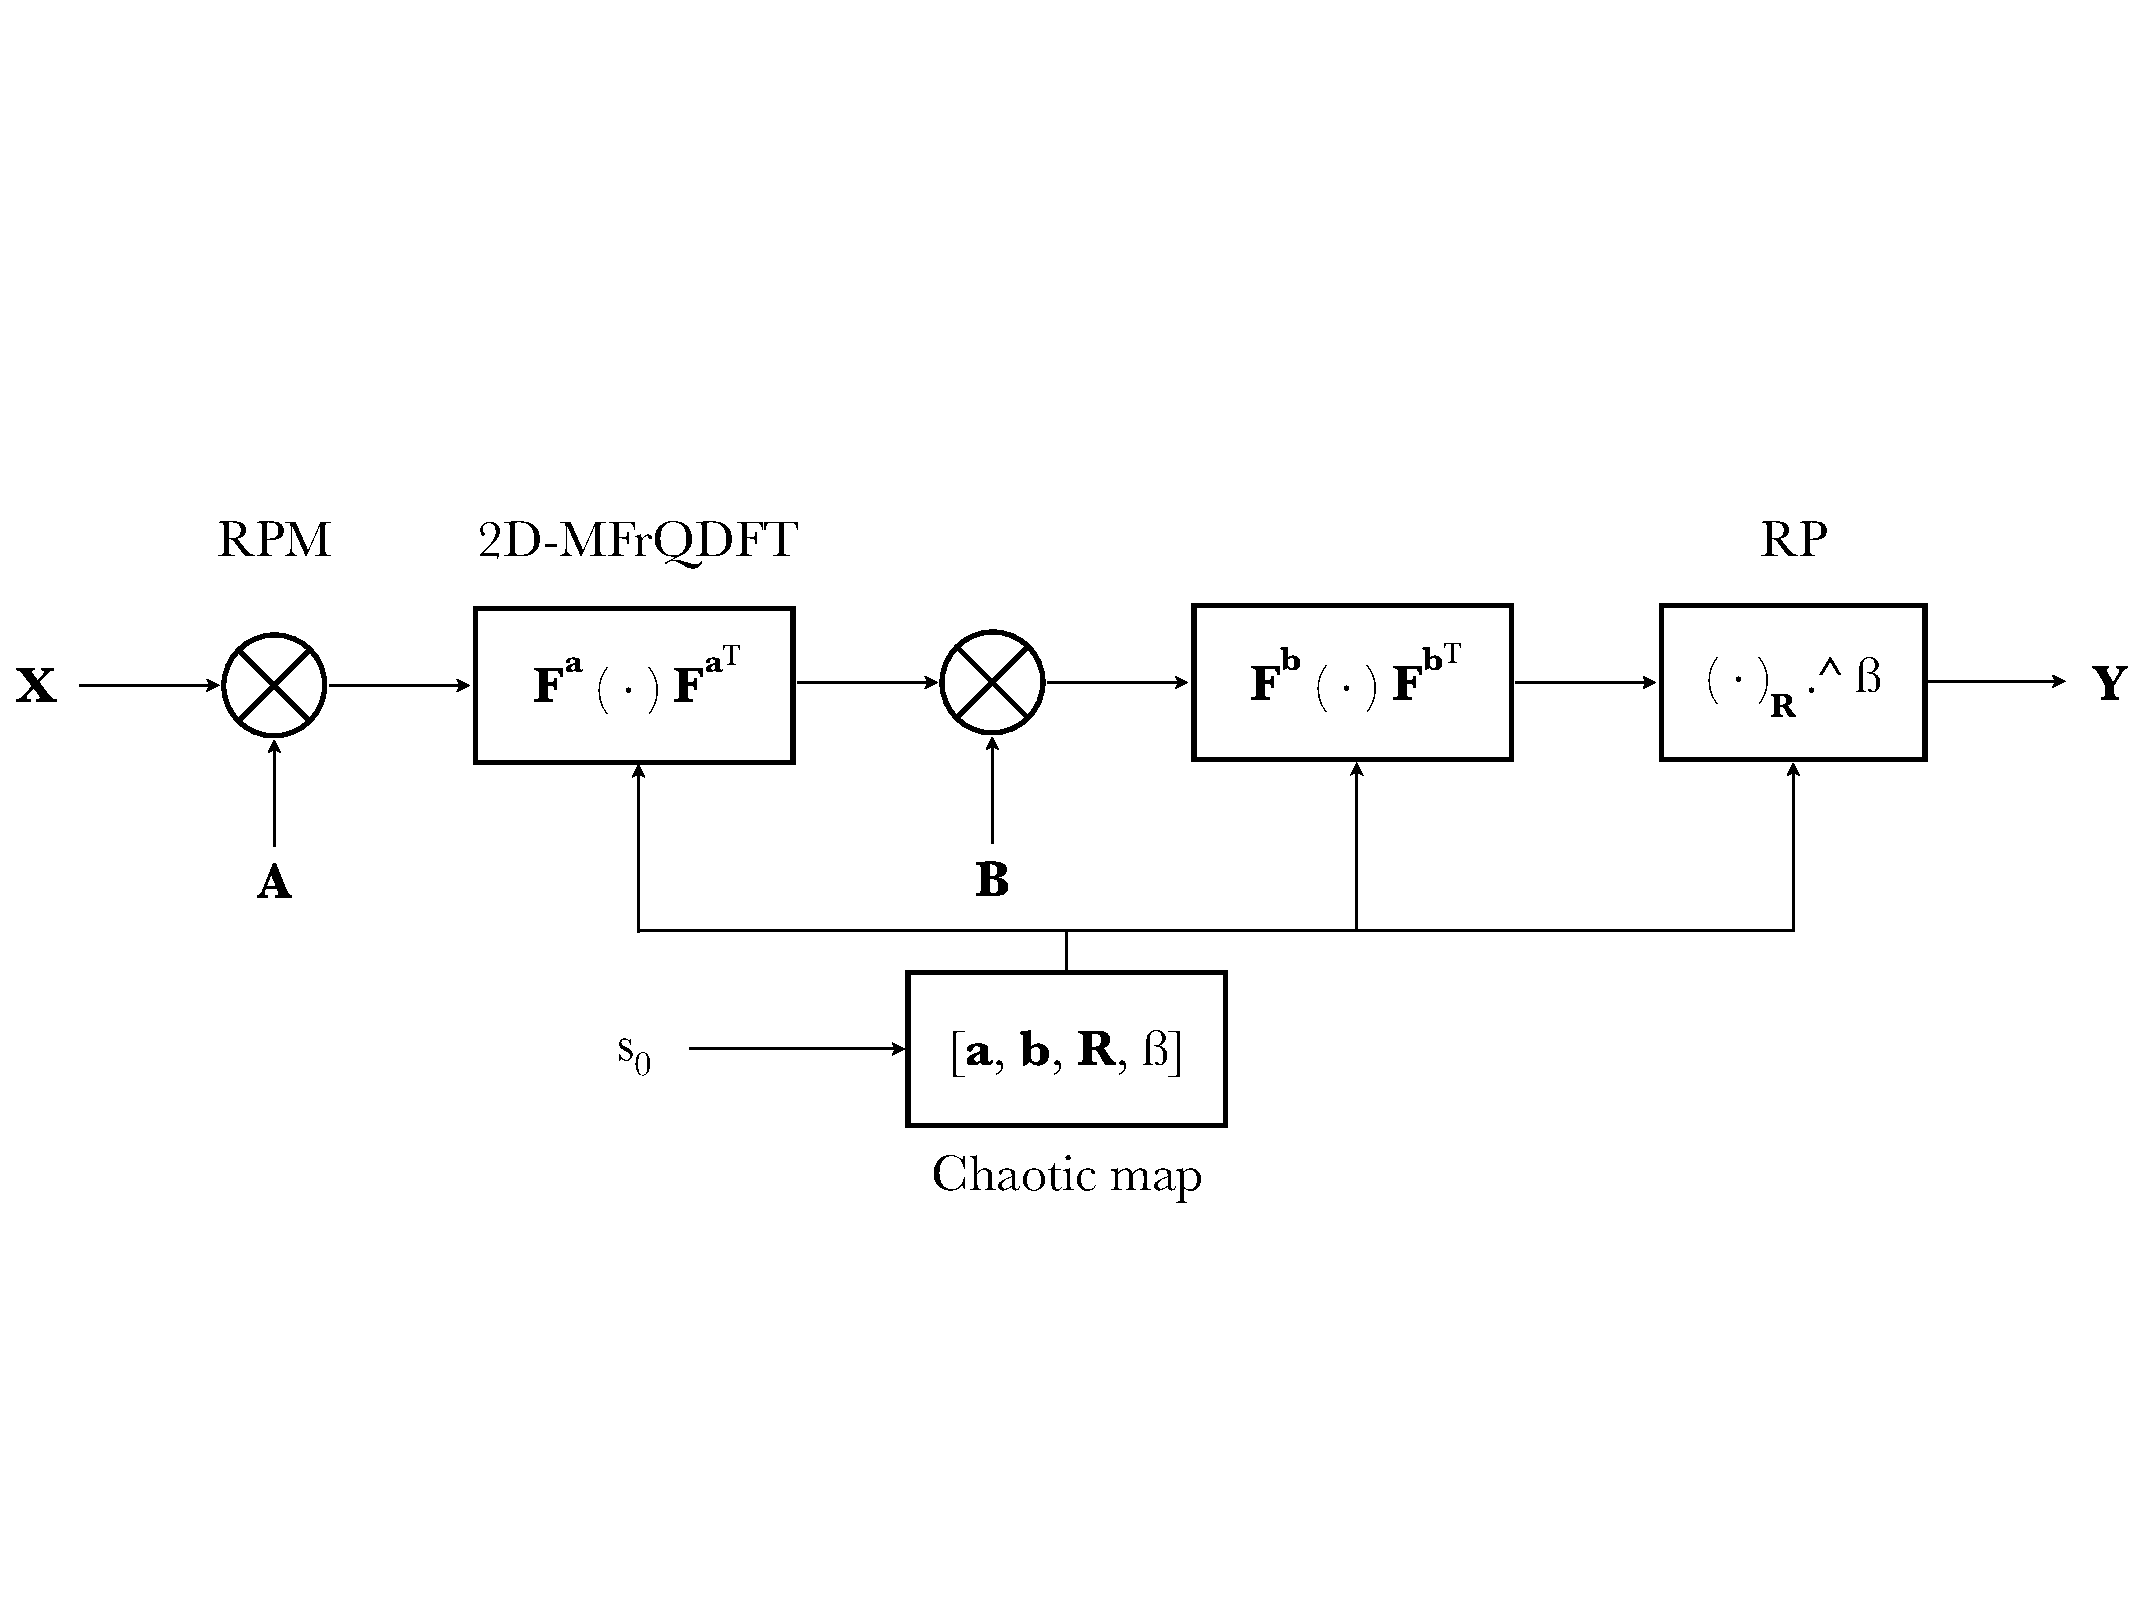
\includegraphics[width=0.9\linewidth]{Figures/esquema_EN.pdf}
\caption{Proposed encryption scheme, exploring the 2D-MFrQDFT.}
\label{fig:cifragem}
\end{figure*}

\begin{figure*}
\centering
\subfloat[\label{fig:ciphered01}]{
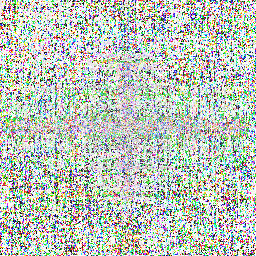
\includegraphics[width=0.2\linewidth]{Figures/sage_Encrypted_image.png}
}~
\subfloat[\label{fig:ciphered02}]{
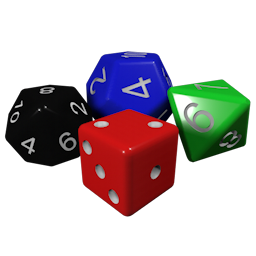
\includegraphics[width=0.25\linewidth]{Figures/Decrypted_image_error_0.png}
}~
\subfloat[\label{fig:ciphered03}]{

\includegraphics[width=0.2\linewidth]{Figures/sage_Decrypted_image_error_minus1dot6.png}
}~
\caption{(a) Encrypted image. (b) Image decrypted with the correct key $ s_0 $. (c) Image decrypted with the wrong key $ \widetilde{s_0} = s_0 + \epsilon $, with $ \epsilon = -1{,}6 \cdot 10^{-80} $.}
\end{figure*}

\subsection{Encryption scheme using MFrQDFT}

The chosen implementation for the PNG image encryption algorithm mixed a block of random-phase modulation (RPM, also called phase mask in \cite{chen2018multiple} and \cite{singh2008optical}) and multiple-parameter transform. As suggested by \cite{hsue2018enhancing}, a non-linear step of random power is also used. Fig. \ref{fig:cifragem} depicts the system building blocks.

The plaintext image is initially converted into a quaternion matrix $ \mathbf{X} $, which is input to a 2-round processing with RPM $ + $ 2D-MFrQDFT. The random-phase modulation consists of element-wise multiplication by a matrix of random unit quaternions. This role is fulfilled by matrices $ \mathbf{A} $ and $ \mathbf{B} $ in Fig. \ref{fig:cifragem}. The \textit{inverse} RPM (in decryption) is achieved using the \textit{conjugate} of the matrix used during encryption.

The random-power block (RP) is the final step in the encryption method. It creates non-linearity by raising randomly selected entries of the matrix $ \mathbf{X} $ to a random parameter $ \beta \in \ ]0,1[$. This selection is performed by a binary matrix $ \mathbf{R} $, so that the output of the RP block to an input quaternions matrix $ \mathbf{M} $ is
\begin{equation}
%\label{key}
\text{RP}(\mathbf{M})_{i,j} =
\begin{cases}
(\mathbf{M}_{i,j})^\beta & \text{if } \mathbf{R}_{i,j} = 1, \\
\mathbf{M}_{i,j} & \text{if } \mathbf{R}_{i,j} = 0.
\end{cases}
\end{equation}
During decryption, one must use the same matrix $ \mathbf{R} $ and an exponent $ \beta^{-1} $.

A chaotic map was used to generate a pseudorandom sequence $ \mathbf{s} $ of numbers between 0 and 1, from which all of the encryption parameters were drawn: the fractional order vectors $ \mathbf{a} $ and $ \mathbf{b} $ of the two 2D-MFrQDFTs, the parameter $ \beta $ and the matrix $ \mathbf{R} $\footnote{For each entry $ \mathbf{R}_{i,j} $, a corresponding element $ s_k $ of $ \mathbf{s} $ was taken and $ \mathbf{R}_{i,j} $ was set to 1 if and only if $ s_k > 0{,}5 $, $ \mathbf{R}_{i,j} = 0 $ otherwise.} for the RP block. The random-phase modulation matrices were produced beforehand and could be left public in the scheme documentation. The encryption of a $ 256 \times 256 $-pixels image, therefore, requires a sequence of length $ 256 + 256 + 256^2 + 1  $. The secret key consists of the seed $ s_0 $ of the chaotic map, a floating point variable between 0 and 1.
%It is clear how the key space and the scheme security depend on the seed floating-point precision and the chosen chaotic map randomness.
As a consequence, the key space is determined by the smallest deviation $ \epsilon $ from $ s_0 $ so that, using the wrong key $ \widetilde{s_0} = s_0 \pm \epsilon $ in decryption, it still leads to a noisy image without any detectable trace of original information.

The key space dimension, denoted by $ [K] $, is the ratio between the range of all possible keys and the range of wrong keys \textit{which still lead to partial image reconstruction}. The latter is $ [s_0 - \epsilon, s_0 + \epsilon] $, following the previous definition of $ \epsilon $. Since $ s_0 \in \ ]0,1[ $,
\begin{equation}
%\label{key}
[K] = \frac{1 - 0}{s_0 + \epsilon - (s_0 - \epsilon)} = \frac{1}{2 \epsilon}.
\end{equation}

When testing the encryption scheme, the \textit{tent map} \cite{singh2008optical} was chosen as tool for generating the $ \mathbf{s} $ sequence; it is recursively defined as
\begin{equation}
%\label{key}
s_{n+1} =
\begin{cases}
\gamma s_n & \text{if } 0 \leq s_0 < 0{.}5, \\
\gamma(1 - s_n) & \text{if } 0{.}5 \leq s_0 \leq 1.
\end{cases}
\end{equation}
with $0 <  \gamma \leq 2 $.

The tent map parameters were set to $ s_0 = 0{.}3 $ and $ \gamma = 1{.}8 $, for no particular reason other than obeying the range of values for chaotic behaviour. The proposed encryption algorithm was used on the image in Fig. \ref{fig:dice}, what yielded the ciphered output in Fig. \ref{fig:ciphered01}.

In order to evaluate the key space dimension, the ciphered image was decrypted using keys $ \widetilde{s_0} = s_0 \pm \epsilon $ for different values of $ \epsilon \in [-10 \times 10^{-80}; 10 \times 10^{-80}]$, with the aid of multiple precision tools provided by the \textit{RealField} class in the SageMath software. By the end of each decryption, it was computed the MSE between the supposedly recovered image and the original one, what is plotted in Fig. \ref{fig:MSE}. The graph does not change smoothly because each tweak in $ s_0 $ propagates along the whole sequence $ \mathbf{s} $, what affects randomly all the decryption parameters. This is, of course, consequence of the nature of a chaotic map. As shown in the graph, the smallest MSE (still using wrong keys, with $ \epsilon \neq 0 $) was 39dB, obtained with $ \epsilon = -1{,}6 \times 10^{-80} $.

Fig. \ref{fig:ciphered02} and \ref{fig:ciphered03} show the decrypted images using $ \epsilon = 0 $ and $ \epsilon = -1{,}6 \times 10^{-80} $, respectively. It can be seen that the wrong key which caused the smallest MSE still produced a seemingly random PNG image, a desirable property for an encryption scheme. Since the smallest deviation used in this test was $ 0{,}83 \times 10^{-80} $, it follows that the key space dimension is, at least, equal to
\begin{equation}
%\label{key}
[K] = \frac{1}{2 \times 0{,}83 \times 10^{-80}} \approx 6{,}0 \times 10^{79},
\end{equation}
what means the key length must be
%o que significa que cada chave deve ter comprimento de
\begin{equation}
%\label{key}
\lceil 79 \log_2 10 \rceil = 263\text{ bits},
\end{equation}
a value greater than 256 bits, assumed to be appropriate for symmetric encryption schemes, by information security reports such as ECRYPT \cite{smart2018algorithms}. It is also clear from these computations and Fig. \ref{fig:ciphered03} how sensitive the scheme is to small key changes: the smallest modification within the precision of $ 10^{-80} $ in the seed $ s_0 $ was enough to provide a completely noisy decrypted image (cf. Fig. \ref{fig:ciphered03}). The high key sensitivity is also indicated by the sharp dip in the MSE $\times $ Error graph in Fig. \ref{fig:MSE}.
%, \'e um tamanho de chaves apropriado para manter sistemas de cifra sim\'etrica em uso por um per\'iodo estimado de 30 a 50 anos.
%.
%
%%A Fig. \ref{fig:RPM} ilustra a oculta\c c\~ao gradual de informa\c c\~ao visual, ao menos nos pixels n\~ao-nulos, ap\'os cada itera\c c\~ao do bloco de RPM. A cada itera\c c\~ao, uma matriz aleat\'oria diferente \'e usada.
%
\begin{figure}
\centering
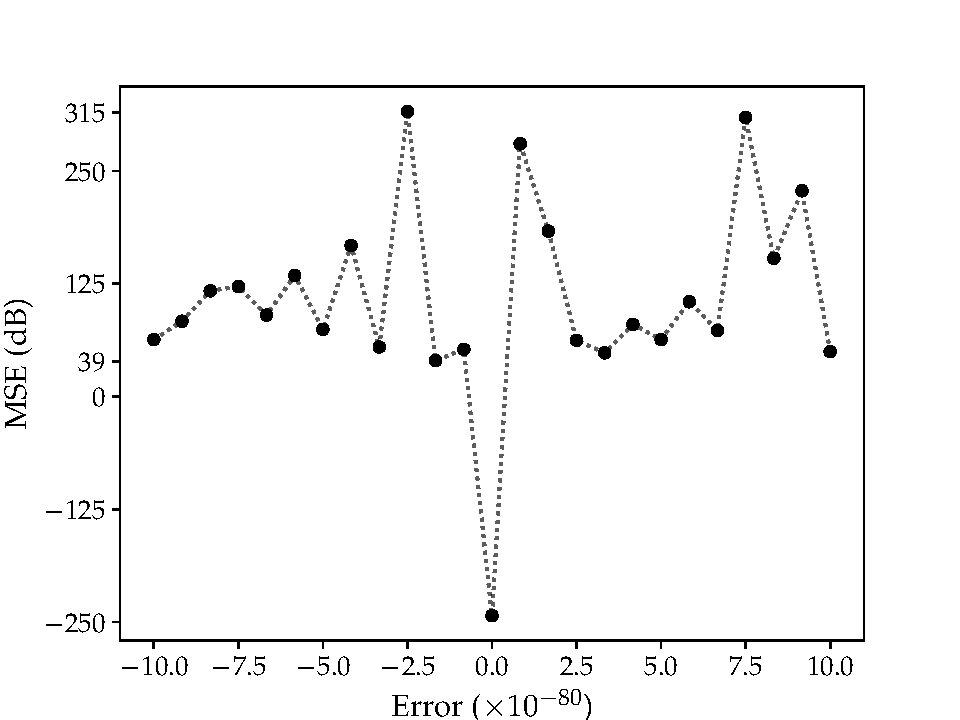
\includegraphics[width=10cm]{Figures/MSEdb_FrQDFT_EN.pdf}
\caption{Mean squared error, in dB, between the original and the decrypted images as function of the key error $ \epsilon $.}
\label{fig:MSE}
\end{figure}
%

Such an encryption scheme would not only be safe against brute-force attacks, given its key space dimension, but also known-plaintext attack. The reason for this is the non-linearity provided by the random-power block, as argued intensely by Hsue \cite{hsue2018enhancing}. Resistance to chosen-plaintext attacks, however, is not guaranteed, although simple adjustments could be done in future works to address this problem: the vector of fractional orders $ \mathbf{a} = \{ a_0, a_1, \dots, a_{N-1} \} $ could be made dependent on both the plain image and external parameters (such as the secret seed $ s_0 $). Such tweak in the algorithm would block the extraction of information from comparing chosen plain images with their encrypted counterparts \cite{chai2019color, hu2017chaotic, murugan2016image}, making the scheme resistant to chosen-plaintext and chosen-ciphertext attacks \cite{wang2012novel}; with resistance also to the weaker attacks of brute-force and known-plaintext.

Alongside the investigation of key space dimension and sensitivity, histogram analysis play an important role in describing the performance of encryption schemes. A practical cipher should present an output symbol distribution ideally independent from the cleartext, so that no information is leaked through histogram visualization  \cite{zhang2014symmetric}.
% "An ideal encrypted image should have a
% uniform and completely different histogram against the plain-image for preventing the adversary from extracting any mean-
% ingful information from the fluctuating histogram of the cipher-image." (zhang2014symmetric)
In the case of a PNG image, four histograms are drawn, one for each layer. Fig. \ref{fig:testing_hist} depicts a test PNG image split into its color and opacity components and the corresponding histograms, both prior and after encryption. A group of 13 $ 256\times 256 $-pixels PNG images were encrypted using the proposed method and the histograms of the ciphered output were collected, what is shown in Fig. \ref{fig:allhistograms}. No matter how diverse the input images may be, the histograms present continuously the same profile, what indicates decoupling of information between plain and ciphered images. Although a deeper study on the properties and safety standards of the proposed encryption scheme is needed for full description of its capacity, the analysis presented fit in the scope of this paper and fulfill the goal of presenting the MFrQDFT with a clear and illustrative application.
%{\color{blue}Each image was ciphered using one of the following randomly defined keys (IMPLEMENTAR): $s_0 = $}. % For quantity analyses of each key, we employ variances of histograms to evaluate uniformity of ciphered images. The low-
% er value of variances indicates the higher uniformity of ciphered images. We also calculate the two variances of ciphered
% images which are encrypted by different secret keys on the same plaintext image. The closer of the two values of variances
% indicates the higher uniformity of ciphered images when the secret keys are varying. The variance of histograms is presented
% as follows:

%Histogram analysis: point out that the conversion from float to int, used prior to histogram-making, did not incur in information loss, because the MSE between the original image and the decrypted, AFTER CONVERSION, was
%MSE:  7.380345314385882e-25
%MSEint:  7.380345314385882e-25


\newcommand{\constlength}{0.33}

\begin{figure}[htbp]
\centering
\subfloat[]{
\includegraphics[width=0.3\linewidth]{Figures/alphatest_resized_decrypted.png}}~
\subfloat[]{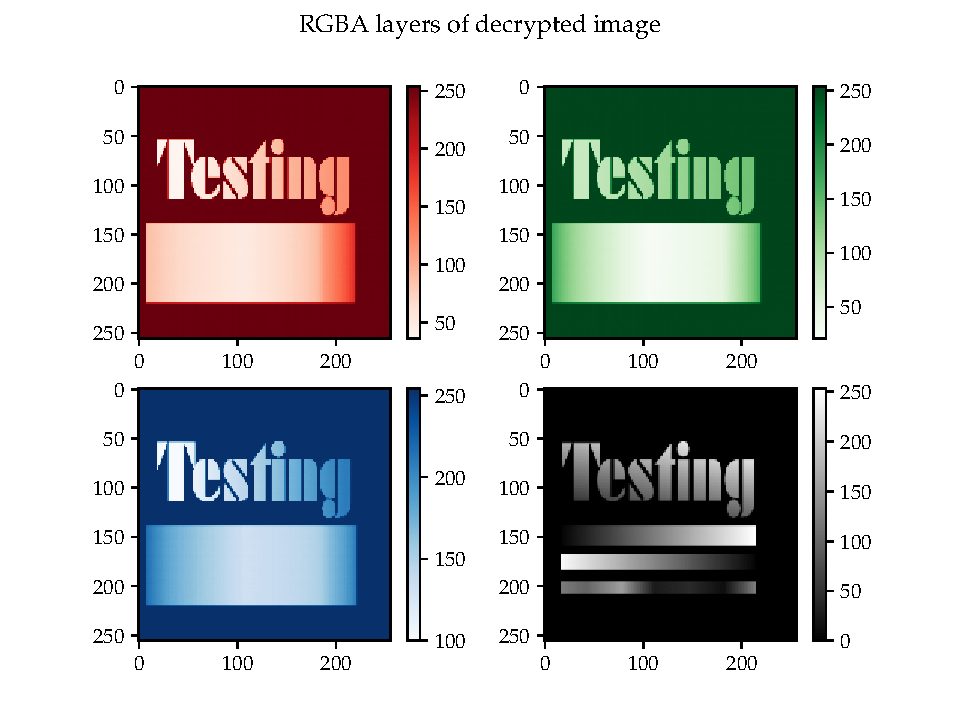
\includegraphics[width=\constlength\linewidth]{Figures/alphatest_resized_decrypted_RGBA_layers.pdf}}~
\subfloat[]{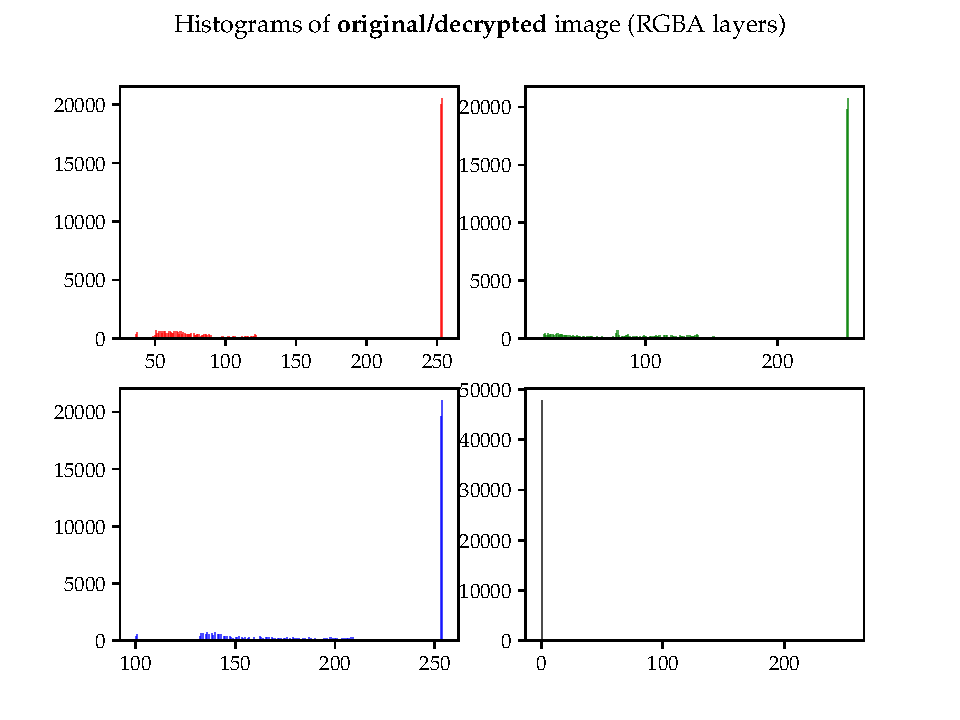
\includegraphics[width=\constlength\linewidth]{Figures/alphatest_resizeddecrypted_histograms.pdf}}\\
\subfloat[]{
\includegraphics[width=0.25\linewidth]{Figures/alphatest_resized_encrypted_img.png}}~
\subfloat[]{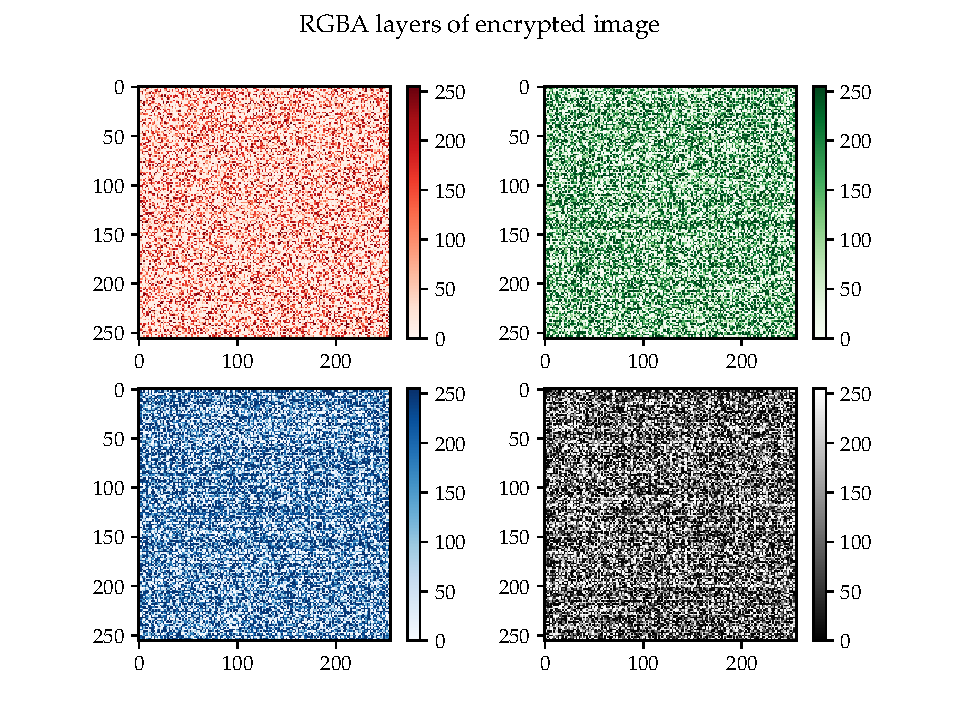
\includegraphics[width=\constlength\linewidth]{Figures/alphatest_resized_encrypted_RGBA_layers.pdf}}~
\subfloat[]{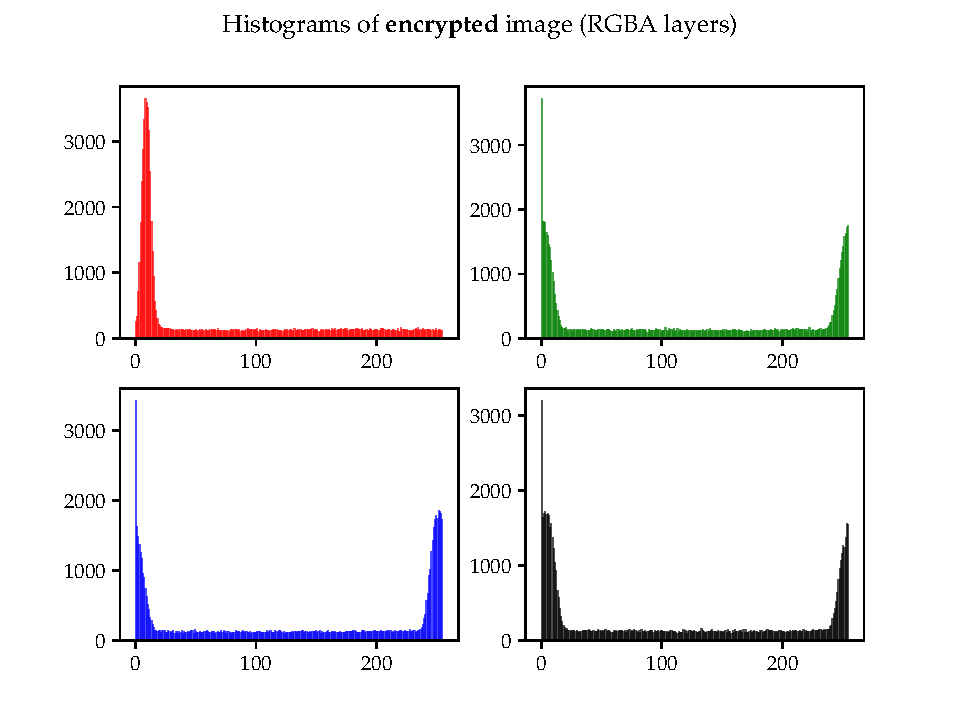
\includegraphics[width=\constlength\linewidth]{Figures/alphatest_resized_encrypted_histograms.pdf}}
\caption{(a) Test image in PNG format, with 256$ \times $256 pixels. (b) Color and opacity layers of the \textit{decrypted} image (which coincides with the original in (a)). (c) Histograms of each layer of the \textit{decrypted} image. (d) Encrypted image, in PNG format. (e) Color and opacity layers of the \textit{encrypted} image. (f) Histograms of each layer of the \textit{encrypted} image.}
\label{fig:testing_hist}
\end{figure}

\newcommand{\fixedlength}{0.32}
\newcommand{\smallerlength}{0.15}
\begin{figure}[htbp]
\centering
\subfloat[]{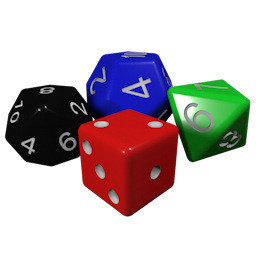
\includegraphics[width=\smallerlength\linewidth]{Figures/dice_256x256_decrypted.png}}~
\subfloat[]{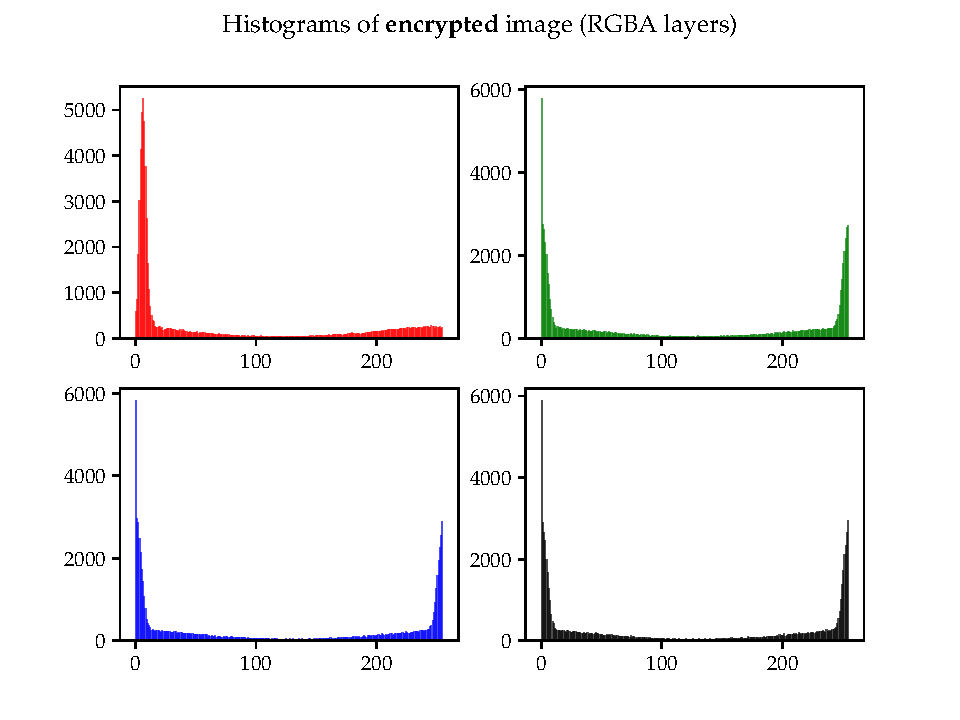
\includegraphics[width=\fixedlength\linewidth]{Figures/dice_256x256_encrypted_histograms.pdf}}~
\subfloat[]{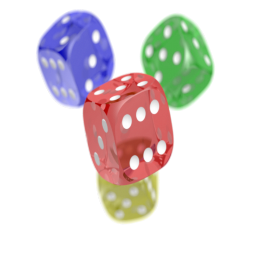
\includegraphics[width=\smallerlength\linewidth]{Figures/another_dice_resized_decrypted.png}}~
\subfloat[]{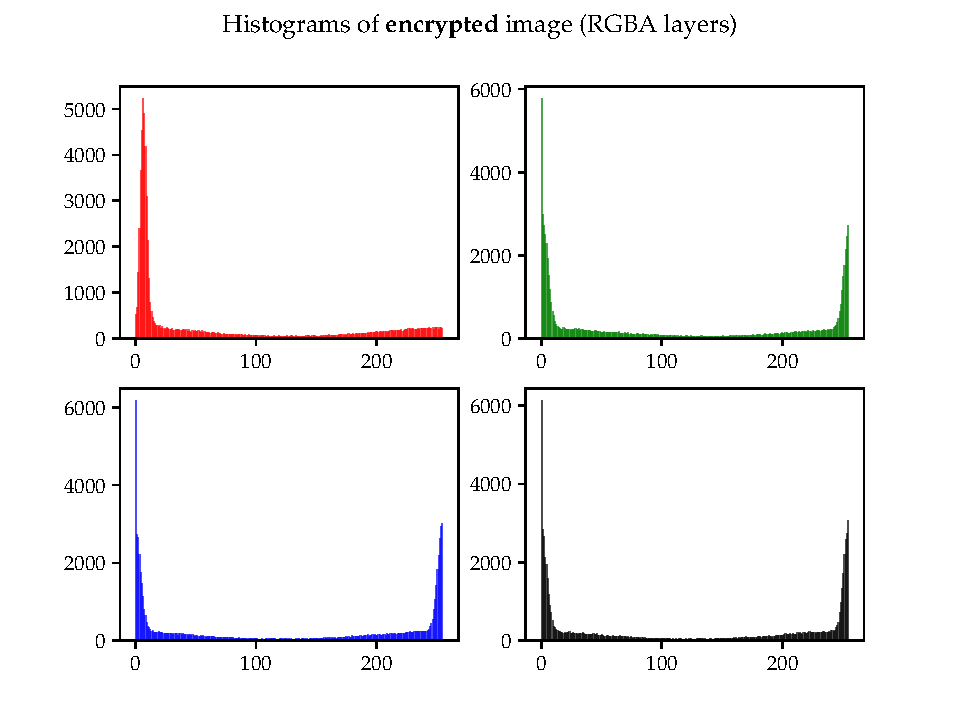
\includegraphics[width=\fixedlength\linewidth]{Figures/another_dice_resized_encrypted_histograms.pdf}}\\
\subfloat[]{\includegraphics[width=\smallerlength\linewidth]{Figures/candle_resized.png}}~
\subfloat[]{\includegraphics[width=\fixedlength\linewidth]{Figures/candle_encrypted_histograms.pdf}}~
\subfloat[]{\includegraphics[width=\smallerlength\linewidth]{Figures/pipe_resized.png}}~
\subfloat[]{\includegraphics[width=\fixedlength\linewidth]{Figures/pipe_encrypted_histograms.pdf}}\\
\subfloat[]{\includegraphics[width=\smallerlength\linewidth]{Figures/dog_resized.png}}~
\subfloat[]{\includegraphics[width=\fixedlength\linewidth]{Figures/dog_encrypted_histograms.pdf}}~
\subfloat[]{\includegraphics[width=\smallerlength\linewidth]{Figures/parrot_resized.png}}~
\subfloat[]{\includegraphics[width=\fixedlength\linewidth]{Figures/parrot_encrypted_histograms.pdf}}\\
\subfloat[]{\includegraphics[width=\smallerlength\linewidth]{Figures/colorparrots_resized.png}}~
\subfloat[]{\includegraphics[width=\fixedlength\linewidth]{Figures/colorparrots_encrypted_histograms.pdf}}~
\subfloat[]{\includegraphics[width=\smallerlength\linewidth]{Figures/bouquet_resized.png}}~
\subfloat[]{\includegraphics[width=\fixedlength\linewidth]{Figures/bouquet_encrypted_histograms.pdf}}
%\caption{Legenda.}
\end{figure}

\stepcounter{figure}
\begin{figure}[htbp]
\centering
\ContinuedFloat
\subfloat[]{\includegraphics[width=\smallerlength\linewidth]{Figures/switzerland_resized.png}}~
\subfloat[]{\includegraphics[width=\fixedlength\linewidth]{Figures/switzerland_encrypted_histograms.pdf}}~
\subfloat[]{\includegraphics[width=\smallerlength\linewidth]{Figures/london_resized.png}}~
\subfloat[]{\includegraphics[width=\fixedlength\linewidth]{Figures/london_encrypted_histograms.pdf}}\\
\subfloat[]{\includegraphics[width=\smallerlength\linewidth]{Figures/russia_resized.png}}~
\subfloat[]{\includegraphics[width=\fixedlength\linewidth]{Figures/russia_encrypted_histograms.pdf}}~
\subfloat[]{\includegraphics[width=\smallerlength\linewidth]{Figures/globe_resized.png}}~
\subfloat[]{\includegraphics[width=\fixedlength\linewidth]{Figures/globe_encrypted_histograms.pdf}}\\
\subfloat[]{\includegraphics[width=\smallerlength\linewidth]{Figures/phones_resized.png}}~
\subfloat[]{\includegraphics[width=\fixedlength\linewidth]{Figures/phones_encrypted_histograms.pdf}}
\caption{Set of 13 PNG test images, 256$ \times $256 pixels, alongside the histograms of each layer (colors and opacity) of their encrypted version. Images downloaded from the online free database \texttt{https://purepng.com/}, under CC0 license.}
\label{fig:allhistograms}
\end{figure}

Finally, as stated at the beginning of the paper, there are a multitude of studies on image encryption, each addressing particular aspects and problems. Therefore, it is adequate to acknowledge the position of this proposed encryption algorithm in the literature landscape. Without providing an extensive and complete analysis, for lack of space, some remarks can be done. The key space dimension in related works vary from circa $ 10^{54} $, around 160 bits, in a work by Wang \textit{et al.} with flexible key space \cite{wang2015novel}, to more than 400 bits, in a paper by Zhang \textit{et al.} \cite{zhang2015new}, an interval which includes the 260 bits of the proposed algorithm. Regarding time of encryption, Wang \textit{et al.} \cite{wang2015novelchaotic} used Arnold cat map and dynamic random growth to obtain large running speed of the encryption and decryption algorithm. This is an aspect our proposed scheme is not optimized for, although great improvement in processing time can be achieved if the eigenvector and eigenvalue matrices of the QDFT are stored in the memory, taking the eigendecomposition out of the encryption process. As a final comment, the main advantages of the scheme proposed in this paper are its modularization, the holistic processing of color images with opacity layer, the lack of long iterations and the ease to describe, comprehend and implement.

\section{Conclusions}
\label{sec:conclusao}
This paper investigated the eigenstructure of the quaternion discrete Fourier transform. Although quaternion matrix decomposition is a challenging topic, the problem for the QDFT was solved by proving that this transform and the DFT share symmetric eigenvectors, what allowed for the construction of an orthogonal eigenbasis of the QDFT, using Hermite--Gaussian-like DFT eigenvectors \cite{de2017discrete}. This result led to the definition of a fractional QDFT, which was proven to hold properties similar to those of the FrDFT, its complex-valued counterpart.

The FrQDFT was further generalized by introducing the MFrQDFT, a multiple-parameter version. Exploring the 4D nature of quaternions, a holistic encryption scheme for color images with opacity layer was proposed, as an illustrative application of the 2D-MFrQDFT, and shown to provide satisfactorily large key space and key sensitivity, resistance to known-plaintext attack and ease of description and implementation. Future works could possibly expand this analysis and address whether some hypercomplex image moments, such as ternary radial harmonic Fourier moments and quaternion polar harmonic \cite{wang2019ternary,wang2018quaternion}, could be used for image encryption, eventually in specific scenarios and applications.

\section{Acknowledgments}
This work has been supported by CNPq (309598/2017-6, 409543/2018-7) and CAPES.

%
\section*{Appendix}
%\subsection{Brief introduction to the quaternion algebra}

The quaternions form an associative division ring invented by William Hamilton in 1843 \cite{hamilton1848xi}, as the first non-commutative algebra in history. It consists of the set  $ \mathbb{H} $ of numbers $ q = a + b \qi + c \qj + d \qk $, with $ a,b,c,d \in \mathbb{R} $ and $ \qi^2 = \qj^2 = \qk^2 = -1 $, along with usual multiplication and addition. The product between imaginary units $ \qi,\qj,\qk $, however, follow the rule in Fig. \ref{fig:quatmult}, e.~g. $ \qk \qi = \qj $ and $ \qk \qj = -\qi $. As a result, quaternion multiplication is non-commutative.

The real and vector parts of a quaternion $ q = a + b \qi + c \qj + d \qk $ are defined as $ \mathcal{S}(q) = a $ and $ \mathcal{V}(q) = b \qi + c \qj + d \qk $. A quaternion $ v $ is said to be \textit{pure} if and only if $ \mathcal{S}(v) = 0 $; it is a \textit{unit quaternion} whenever $ |v| \overset{\Delta}{=} \sqrt{a^2 + b^2 + c^2 + d^2} = 1 $. The conjugation of $ q $ is $ \bar{q} \overset{\Delta}{=} \mathcal{S}(q) - \mathcal{V}(q) $. There is an Euler form for quaternions, similar to the known complex case, given by
\begin{equation}
\label{eq:euler}
q = |q| e^{\qmu \theta} = |q|\cos \theta + |q|\qmu \sin \theta,
\end{equation}
where $ \qmu = \mu_1 \qi + \mu_2 \qj + \mu_3 \qk$ is a unit pure quaternion. If one computes $ \qmu^2 $, the result will be
\begin{equation}
%\label{key}
\begin{aligned}
\qmu^2 & = (\mu_1 \qi + \mu_2 \qj + \mu_3 \qk) (\mu_1 \qi + \mu_2 \qj + \mu_3 \qk) \\
& = -\mu_1^2 + \cancel{\mu_1\mu_2 \qk} - \cancel{\mu_1\mu_3 \qj} \\
& \quad - \mu_2^2 - \cancel{\mu_2\mu_1 \qk} + \cancel{\mu_2\mu_3 \qi} \\
& \quad -\mu_3^2 - \cancel{\mu_3\mu_1 \qj} - \cancel{\mu_3\mu_2 \qi} \\
&= -1,
\end{aligned}
\end{equation}
from which follows that any unit pure quaternion is a square root of unity. This property justifies the isomorphism between the set $ \mathbb{C}_{\qi} $ of complex numbers $ a + b\qi $ and the set $ \mathbb{C}_{\qmu} \subset \mathbb{H}$ of quaternions $ a + b\qmu $, which have vector part parallel to $ \qmu $. For a thorough introduction to quaternions and their application to signal processing, the reader may refer to \cite{zhang1997quaternions,ell2014quaternion,flamant2017time}.

\begin{figure}
\centering
\includegraphics[width=5cm]{Figures/quaternion_multiplication.pdf}
\caption{Diagram illustrating the multiplication rule between quaternion imaginary units $ \qi $, $ \qj $ and $ \qk $.}
\label{fig:quatmult}
\end{figure}


\chapter{Quaternion graph signal processing}
\label{ch:QGSP}

% Numerous studies in the last decade have contributed to establish graph signal processing as a fruitful and promising field of research. Sharing the main aim of generalizing principles and techniques of classical signal processing to the context of network-based signal domain~\cite{ortega2018graph}, two main approaches have risen through the recent years and they constitute the root of GSP. The first one --- that presented in section \ref{sec:GSPintro} --- stems from algebraic signal processing, using the weighted adjacency matrix and elementary block. This approach deals with signals defined on both directed and undirected graphs, with both real- and complex-valued edge weights~\cite{sandryhaila2014big}. The second one is based on spectral graph theory and focuses only on signals defined on undirected graphs with real-valued edge weights, using the graph Laplacian matrix to build the signal space~\cite{shuman2013emerging}.

% Recent formulations of GSP have unified the two by stating that, regardless of the graph matrix at hand (Laplacian, adjacency, and others \cite{chen2018shift, dees2019unitary}), all GSP tools emerge from the choice of unit graph shift operator. Similarly to classical DSP, the shift operator generates the eigenbasis of linear and shift invariant filters ("linear and time invariant", in the discrete-time domain).
% As shown in section \ref{sec:GSPintro}, the eigendecomposition of this operator plays a central role in GSP.

% \begin{figure}
% \centering
% \includegraphics[width=0.3\linewidth]{Figures/signal_duher_graph_2.pdf}
% \caption{Example of graph signal. The graph edges capture similarity or interdependency relationship between samples. What new possibilities are created when the edges carry quaternion weights? Source: the author.}
% \label{fig:duher}
% \end{figure}

Section \ref{sec:GSPintro} presented the motivation and fundamentals of graph signal processing, while Chapter THIS delved into the exploration of a fractional graph shift. The current chapter will extend even more the borders of the field.

The problem at hand, when applying GSP, will define the characteristics of the underlying graph, e.g. whether using real or complex edge weights, directed or undirected graphs. The exploration of new algebras for the edge weights, however, open new possibilities for tools and applications, similarly to what happened in electrical engineering when modeling electric signals using complex-valued functions. The engineers were able to explore with variables that, carrying two sources of information (amplitude and phase), have proven more suitable to the visualization and manipulation of harmonic functions than if only real-valued functions were employed. That was also the reasoning of Ortoloni and Uncini \cite{ortolani2016quaternion}, when they proposed the study of discrete-time signal processing with \emph{quaternion-valued} samples.

As did Jiang et al. \cite{jiang2013frequency} when benefiting from using quaternion-valued adaptive filters to tackle the problem of wind profile prediction (3D signals of wind direction at each point in the Euclidian space), or Flamant et al. \cite{flamant2018complete} that created a framework for time-frequency analysis of bivariate signals using quaternions, the hypothesis of this thesis is that the study of GSP with quaternion values may reveal both theoretical and practical implications of great interest. Such generalization has the appeal to allow not only for the analysis of discrete-time three- or four-dimensional signals (as in quaternion discrete signal processing), but also for the exploration of interrelations that capture there higher dimensions (i.e. edge weights). The tools arising from the consequences of such investigation is from now on referred to as QGSP (quaternion graph signal processing).

\section{Laying the foundations for QGSP}

We will define QGSP simply as the development and application of GSP tools to the context of quaternion-valued signals and graph edge weights. That is, we extend the usual complex-valued case to

\begin{align}\label{eq:qgsp_defs}
\mathcal{G} &= \{\mathcal{V}, \mathbf{A}\}  \ | \ \mathbf{A} \in \mathbb{H}^{n \times n}, \notag \\
s: &\ \mathcal{V} \rightarrow \mathbb{H}^{n \times 1} \ | \ s(v_i) = s_i,
\end{align}

As such, a few milestones were set to be conquered in order to fully establish QGSP:
\begin{itemize}
\item An algorithm to compute the direct and inverse (quaternion) graph Fourier transforms,
\item A definition of frequency ordering,
\item A method to design filters tailored to certain problems.
\end{itemize}

\subsection{On the inversion of the eigenvector matrix}

The inversion of quaternion matrices have been tackled by many researchers, yielding a few algorithms aiming at solving it. \red{(INSERT REFERENCES)} All seemed too costly to practical use in medium to large graphs. Based on theorems \ref{th:equiv01} and \ref{th:equiv02},
the algorithm \ref{alg:qinv} is proposed to provide a reasonable balance between processing speed and broad applicability.

The reasoning goes as follows. According to theorem \ref{th:equiv02}, a necessary and sufficient condition for the invertibility of a matrix $\mathbf{V} \in \mathbb{H}^{n \times n}$ is the existance of $\rchi^{-1}_{V}$. Moreover, from theorem \ref{th:equiv01}, if $\rchi^{-1}_{V}$ exists and has the form of a complex adjoint matrix, let us say $\rchi_{V}^{-1} = \rchi_{M}$, then it follows that $\mathbf{M} = \mathbf{V}^{-1}$, since the theorem guarantees that
\begin{equation}
\rchi_{V} \rchi_{M} = \rchi_{V} \rchi_{V}^{-1} = \mathbf{I}_{2n \times 2n} = \rchi_{I_{n \times n}}
\Rightarrow \mathbf{V} \mathbf{M} = \mathbf{I}_{n \times n},
\end{equation}
letting $\mathbf{I}_{m \times m}$ be the identity matrix of order $m$\footnote{For simplicity, this notation is slightly loose, representing both a complex- and a quaternion-valued identity matrix, since in both cases their entries have zero-valued or zero-normed imaginary parts.}.

\begin{center}
\begin{algorithm}
\caption{Inversion of quaternion matrices.}\label{alg:qinv}
\SetKwInOut{Input}{input}\SetKwInOut{Output}{output}
\Input{$\mathbf{V} \in \mathbb{H}^{n \times n}$}
\Output{$\mathbf{V}^{-1}$ ou None (vazio).}
$\rchi_{V} \gets \mathrm{complex\_adjoint(\mathbf{V})}$\;

\If{$\mathrm{det}(\rchi_{V}) = 0$}{\Return None}

$\mathbf{U} \gets \mathrm{inverse(\rchi_{V})}$

\If{\textup{\textbf{not}} $\mathrm{has\_complex\_adjoint\_form}(\mathbf{U})$}{\Return None}

$\mathbf{V}^{-1} \gets \mathrm{from\_complex\_adjoint}(\mathbf{U})$

\Return $\mathbf{V}^{-1}$
\end{algorithm}
\end{center}

\section{Example: denoising a quaternion graph signal via QLMS low-pass filtering}

\begin{figure}
	\centering
	\includegraphics[width=0.25\linewidth]{thesis/Figures/uk_graph.png}
	\caption{Graph created using the cities in UK.}
	\label{fig:uk_graph}
\end{figure}

\begin{figure}
	\centering
	\includegraphics[width=0.55\linewidth]{thesis/Figures/uk_graph_kernel.png}
	\caption{Test.}
	\label{fig:uk_graph_kernel}
\end{figure}

\begin{figure}
	\centering
	\includegraphics[width=0.55\linewidth]{thesis/Figures/uk_graph_kernel_noisy.png}
	\caption{Test.}
	\label{fig:uk_graph_kernel_noisy}
\end{figure}

\begin{figure}
	\centering
	\includegraphics[width=0.55\linewidth]{thesis/Figures/uk_graph_filtered.png}
	\caption{Test.}
	\label{fig:uk_graph_filtered}
\end{figure}

\chapter[Considera\c c\~oes finais]{Considera\c c\~oes finais}
\label{ch:others}

Este projeto de tese prop\~oe-se a contribuir com o processamento de sinais quaterni\^onicos, em particular pelo estudo da autodecomposi\c c\~ao de matrizes quaterni\^onicas, sejam elas matrizes de transforma\c c\~oes lineares ou operadores de deslocamento sobre grafos com pesos quaterni\^onicos. O estudo da autoestrutura da QDFT levou a um novo m\'etodo para sua fracionariza\c c\~ao, juntamente com a proposta de uma vers\~ao multiparam\'etrica e um esquema de cifragem de imagens coloridas com camada de opacidade. A decomposi\c c\~ao de matrizes que servem como operadores de deslocamento para sinais sobre grafos deve ser revelada, em parte, pelos estudos conduzidos at\'e o momento, reunindo teoremas relacionando propriedades destas matrizes e de suas complexas adjuntas, bem como sobre a exist\^encia e similaridade entre autovalores de matrizes sobre os quat\'ernios.

Dentre os desafios te\'oricos que permanecem, pode-se listar os seguintes:
\begin{itemize}
\item encontrar classes de grafos com operadores de deslocamento diagonaliz\'aveis. De fato, enquanto um grafo n\~ao-direcionado com pesos reais ou complexos possui um operador de deslocamento sempre diagonaliz\'avel, n\~ao se pode afirmar o mesmo quando os pesos percentem a $ \mathbb{H} $, pois a simetria presente na matriz de adjac\^encia de um grafo quaterni\^onico n\~ao-direcionado n\~ao se transmite \`a sua matriz complexa adjunta. Neste sentido, pretende-se investigar se h\'a classes de grafos com operadores de deslocamento diagonaliz\'aveis, ou se \'e poss\'ivel definir operadores com tal propriedade. Este problema alinha-se com o entendimento de \cite{ortega2018graph}, que observam forte interesse da comunidade em avan\c cos te\'oricos de GSP voltados a \emph{classes espec\'ificas} de grafos.
\item Ainda nesta linha, pode-se investigar se h\'a quaisquer propriedades particulares presentes na classe de grafos quaterni\^onicos que possuem \emph{apenas autovalores reais} (i.~e. cada autoclasse possui apenas um elemento e o grafo possui um n\'umero finito de autovalores). Em GSP, esta propriedade \'e observada, por exemplo, nos grafos n\~ao-direcionados de pesos reais.
\item Por fim, outra quest\~ao de estudo em aberto \'e como definir um ordenamento das frequ\^encias quando os autovetores s\~ao quaterni\^onicos, pois ainda n\~ao est\'a claro se \'e poss\'ivel transpor a interpreta\c c\~ao oriunda da varia\c c\~ao total sobre grafos, em (\ref{eq:var_total}), para o contexto quaterni\^onico.
\end{itemize}
%est\'a o problema de encontrar classes de grafos com operadores de deslocamento diagonaliz\'aveis. De fato, enquanto um grafo n\~ao-direcionado com pesos reais ou complexos possui um operador de deslocamento sempre diagonaliz\'avel, n\~ao se pode afirmar o mesmo quando os pesos percentem a $ \mathbb{H} $, pois a simetria presente na matriz de adjac\^encia de um grafo quaterni\^onico n\~ao-direcionado n\~ao se transmite \`a sua matriz complexa adjunta. Neste sentido, pretende-se investigar se h\'a classes de grafos com operadores de deslocamento diagonaliz\'aveis, ou se \'e poss\'ivel definir operadores com tal propriedade. Este problema alinha-se com o entendimento de \cite{ortega2018graph}, que observam forte interesse da comunidade em avan\c cos te\'oricos de GSP voltados a \emph{classes espec\'ificas} de grafos. Ainda nesta linha, pode-se investigar se h\'a quaisquer propriedades particulares presentes na classe de grafos quaterni\^onicos que possuem \emph{apenas autovalores reais} (i.~e. cada autoclasse possui apenas um elemento e o grafo possui um n\'umero finito de autovalores). Por fim, outra quest\~ao de estudo em aberto \'e como definir um ordenamento das frequ\^encias quando os autovetores s\~ao quaterni\^onicos, pois ainda n\~ao est\'a claro se \'e poss\'ivel transpor a interpre\c c\~ao oriunda da varia\c c\~ao total sobre grafos, em (\ref{eq:var_total}), para o contexto quaterni\^onico.

%\red{Ler estas fontes e comentar \cite{yin2019quaternion, hsu2018quatnet, parcollet2019quaternion}}

%De posse de um acabou\c co b\'asico de an\'alise espectral e filtragem em QGSP, pretende-se implementar os algoritmos e estruturas de dados em \emph{software}.
Um arcabou\c co coeso de QGSP deve encontrar aplica\c c\~oes em cen\'arios envolvendo sinais que guardem informa\c c\~oes em tr\^es ou quatro dimens\~oes, como dados de dire\c c\~ao de fluidos, imagens coloridas ou rota\c c\~oes de objetos no espa\c co tridimensional. O uso de quat\'ernios pode melhorar a performance em alguns problemas que, hoje, s\~ao atacados com GSP tradicional, tal como ocorreu com aplica\c c\~oes de redes neurais convolucionais \emph{quaterni\^onicas}. Estudos mostraram resultados iguais ou superiores a esquemas com redes convolucionais tradicionais em problemas de processamento e classifica\c c\~ao de imagens coloridas \cite{yin2019quaternion, parcollet2019quaternion}, bem como estima\c c\~ao de pose a partir apenas de imagens em RGB \cite{hsu2018quatnet}. Um exemplo para aplica\c c\~ao de QGSP seria o uso de grafos para predi\c c\~ao de movimento ou compress\~ao de nuvens de pontos (\textit{point clouds}) com informa\c c\~ao espacial e de cor. Em \cite{thanou2016graph}, nuvens de pontos com informa\c c\~ao de cor e posi\c c\~ao no espa\c co 3D s\~ao modeladas como um grafo sobre o qual se define seis sinais distintos (tr\^es de posi\c c\~ao e tr\^es de cor). Utiliza-se de an\'alise espectral para extrair \emph{features} sobre cada um destes sinais, de forma independente, de modo a utiliz\'a-las para estima\c c\~ao de movimento e compress\~ao das nuvens de pontos. Ora, pode-se afirmar sem d\'uvida alguma que tais sinais n\~ao s\~ao independentes e a modelagem utilizando QGSP poderia prover um processamento hol\'istico, eventualmente com maior capacidade de compress\~ao. Em \cite{batabyal2015ugrasp}, os autores representam pontos do corpo humano como v\'ertices de um grafo 3D, com pesos das arestas relacionados \`a dist\^ancia euclidiana entre estes pontos, e utilizam-no para extrair vari\'aveis de entrada para algoritmos de aprendizado de m\'aquina. Cada amostra do sinal sobre o grafo \'e uma tripla ordenada $ s_i = (x_i, y_i, z_i) $, indicando a posi\c c\~ao do v\'ertice no espa\c co. Este sinal, originalmente composto por elementos em $ \mathbb{R}^3 $, \'e representado pelos autores como $ \hat{\mathbf{s}} = [x_1, \dots, x_N, y_1, \dots, y_N, z_1, \dots, z_N] \in \mathbb{R}^{3N}$, ao mesmo tempo em que se define a extens\~ao da matriz $ \mathbf{U} $ de autovetores da Laplaciana: $ \mathbf{U}_g = \text{diag}(\mathbf{U}, \mathbf{U}, \mathbf{U}) $, de modo a se poder utilizar GSP tradicional. O uso de grafos e sinais quaterni\^onicos poderia prover um modelo que naturalmente explora o sinal na sua forma original.
